%%%%%%%%%%%%%%%%%%%%%%%%%%%%%
%Packages are included below, these are akin to libraries in other programming languages. As far as I can tell, there is no reason to reduce the number of packages included in a document. It might compile faster, but overleaf compiles fast so this should not be an issue.
\documentclass[hidelinks,11pt,twoside]{report} %tells the compiler that this is a 'report' style document, and the main font size.


%%%%%%%%%%%%%%%%%%%%%%%%%%%%%%%%%%

\usepackage{setspace} %allows the use of '\doublespace' to set line spacing
\usepackage[english]{babel} %this does a few things e.g. allowing dates to be made by the compiler. probably best not to get rid of it
\usepackage{graphicx} %this allows graphics to be put in easily
\usepackage{float}%this allows you to put them in good places
\usepackage[version=4]{mhchem} %this is good for chemical reactions
\usepackage{epigraph} %citation introduction
\usepackage{blindtext}
\renewcommand{\textflush}{flushepinormal}
\usepackage{adjustbox}   %NEW
\newenvironment{compactepigraph}
  {%
    \par\vspace{0pt}% tighten space above
    \noindent
    \begin{minipage}{0.95\textwidth}%
      \begin{flushright}%
        \small\itshape
  }
  {%
        % end of quote text
        \par\nobreak\vspace{0.3\baselineskip}% small gap
        \noindent\makebox[\linewidth]{\rule{0.4\textwidth}{0.4pt}}% rule
        \par\nobreak\vspace{0.3\baselineskip}% small gap
        \normalfont% switch back to upright
      \end{flushright}%
    \end{minipage}%
    \vspace{0pt}\par% tighten space below
  }

\usepackage{amsmath} %maths package
\usepackage{amssymb} %symbol package
\usepackage{textcomp,gensymb} %more symbols (eg \degree)
\usepackage{colortbl} %good for colouring in cells on a table
\usepackage{rotating} %allows you to rotate graphics
\usepackage{bm} %helps bold things
\usepackage{multirow} %for tables
\usepackage{longtable} %for long tables
\usepackage{booktabs} %more tables
\usepackage{pdfpages} %allows PDFs to be included in document (good if you want to include a pdf in an appendix eg)
\usepackage{caption} %allows captions for graphics
\usepackage[nottoc]{tocbibind} %adds the bibliography to the table of contents
\usepackage{subcaption} %allows subcaption for multiple images in one graphic

\PassOptionsToPackage{hyphens}{url}\usepackage{hyperref}
\usepackage{hyperref} %this is great for putting hyperreferences in the document.
\usepackage[table]{xcolor} %more colouring of tables
\definecolor{Gray}{gray}{0.9} %this defines a colour to be used and gives it a name. This is a colour called 'Gray' it is 'gray' with transparency 0.9

\hypersetup{colorlinks=false} %this stops links being colourful, which makes a report look less professional I believe.
\usepackage[flushleft]{threeparttable}
\usepackage{caption}

\usepackage[letterpaper, top=1in, bottom = 1in, right = 1in]{geometry} %this describes the layout of the document and the margins etc.

\usepackage[labelformat=empty]{caption} % this way, I can have "Figure X" in bold below ech figure

% remove indentation and ensure blank line between paragraphs
%\setlength{\parindent}{0pt}
%\setlength{\parskip}{1em}

\setlength{\parindent}{15pt}
\setlength{\parskip}{0pt}

%\doublespacing %self explanatory
\onehalfspacing

\usepackage{apacite}


\usepackage{pdflscape}   % rotate the page
\usepackage{array}       % better column types
\usepackage{longtable}   % multipage tables
\usepackage{booktabs}
\usepackage{threeparttablex} % longtable-compatible notes
\newcommand{\ra}[1]{\renewcommand{\arraystretch}{#1}}




\usepackage{hyperref}
\usepackage{url}

\usepackage{natbib}

\usepackage{multibib}
\newcites{internet}{Internet References}

\renewcommand{\thefootnote}{\arabic{footnote}}

\usepackage{titlesec}    
 
\titleformat{\chapter}[display]{\normalfont\bfseries}{}{}{\LARGE\thechapter.\ }
   
\titleformat*{\section}{\Large\bfseries}
\titleformat*{\subsection}{\large\bfseries}
\titleformat*{\subsubsection}{\normalsize\bfseries}


\usepackage[dvipsnames]{xcolor}
 
\usepackage[nottoc]{tocbibind}


\usepackage{url}
\PassOptionsToPackage{hyphens}{url}\usepackage{hyperref}


\usepackage{listings}

\usepackage{xcolor}

\usepackage{enumitem}

\usepackage{comment}

\definecolor{codegreen}{rgb}{0,0.6,0}
\definecolor{codegray}{rgb}{0.5,0.5,0.5}
\definecolor{codeblack}{rgb}{0.58,0,0.82}
\definecolor{backcolour}{rgb}{0.95,0.95,0.92}

\lstdefinestyle{mystyle}{
    backgroundcolor=\color{white},   
    commentstyle=\color{codegreen},
    keywordstyle=\color{black},
    numberstyle=\tiny\color{codegray},
    stringstyle=\color{codepurple},
    basicstyle=\ttfamily\footnotesize,
    breakatwhitespace=false,         
    breaklines=true,                 
    captionpos=b,                    
    keepspaces=true,                 
    numbers=left,                    
    numbersep=5pt,                  
    showspaces=false,                
    showstringspaces=false,
    showtabs=false,                  
    tabsize=2
}

\lstset{style=mystyle}

\usepackage{chngcntr}
\usepackage{titling}
\counterwithout{figure}{chapter}
\counterwithout{table}{chapter}

\usepackage{tocloft}
\renewcommand{\cftfigpresnum}{}
\renewcommand{\cftfigaftersnum}{}
\renewcommand{\cfttabpresnum}{}
\renewcommand{\cfttabaftersnum}{}

\cftsetindents{figure}{0em}{3.5em}
\cftsetindents{table}{0em}{3.5em}

\usepackage{tocbasic}

\usepackage[title,toc,titletoc,page]{appendix}
\usepackage{blindtext}


% Format the title for chapters
\titleformat{\chapter}{\normalfont\LARGE\bfseries}{\thechapter.}{20 pt}{\LARGE}
\titlespacing*{\chapter}{0pt}{-20pt}{10pt}


\renewcommand\cfttoctitlefont{\LARGE \bfseries}
\addtocontents{toc}{\vskip -1.5cm}

\renewcommand\cftloftitlefont{\LARGE \bfseries}
\addtocontents{lof}{\vspace*{-6ex}}%


\renewcommand\cftlottitlefont{\LARGE \bfseries}
\addtocontents{lot}{\vspace*{-6ex}}%


% Set up links
\definecolor{light_blue}{rgb}{0.180, 0.188, 0.573}


\hypersetup{
    colorlinks=true,
    linkcolor=blue,    % internal document links
    citecolor=blue,    % citation links
    filecolor=blue,    % file links
    urlcolor=blue      % external urls
}



\usepackage[savewrites,nonumberlist, seeautonumberlist]{glossaries}
\glstoctrue
\newglossarystyle{mystyle}{
  \renewenvironment{theglossary}
    {\begin{longtable}[l]{p{3cm}p{\glsdescwidth}}}
    {\end{longtable}}
  \renewcommand*{\glossaryheader}{%
    \textbf{\glossaryname} \\
    \textbf{Term} & \textbf{Description} \\
    \endhead
  }
  \renewcommand*{\glossentry}[2]{%
    \glsentryitem{##1}\textbf{\glstarget{##1}{\glossentryname{##1}}} &
    \glossentrydesc{##1}\\
  }
  \renewcommand*{\subglossentry}[3]{%
    \glsentryitem{##2}\hspace*{10pt}\glstarget{##2}{\glossentryname{##2}} &
    \glossentrydesc{##2}\\
  }
}

\renewcommand{\glsnamefont}[1]{\textbf{#1}}

\setlength{\cftbeforechapskip}{1.5pt}
\renewcommand\cftchapafterpnum{\vskip2pt}
\renewcommand\cftsecafterpnum{\vskip1pt}
\renewcommand\cftsubsecafterpnum{\vskip1pt}

%toc
\addto{\captionsenglish}{\renewcommand*{\contentsname}{Table of Contents}}
\setlength{\cftbeforetoctitleskip}{20pt}
\setlength{\cftaftertoctitleskip}{60pt} 
%lof
\setlength{\cftbeforeloftitleskip}{0pt} 
\setlength{\cftafterloftitleskip}{40pt} 
%lot
\setlength{\cftbeforelottitleskip}{20pt} 
\setlength{\cftafterlottitleskip}{40pt} 

\setcounter{table}{-1}

\renewcommand{\glossarypreamble}{\vspace*{-10pt}}

\captionsetup[subfigure]{justification=centering}
\captionsetup[subtable]{justification=centering}
\captionsetup[table]{justification=centering}
\captionsetup[figure]{justification=centering}

\makeglossaries

\newglossaryentry{}
{name=XXX, description={XXX}}


%\usepackage{fancyhdr}
%\usepackage{etoolbox}

%\fancypagestyle{fancy}{%
 %\fancyhf{}
%\rhead{Valentine Di Lello}
%\lhead{\leftmark}
%\cfoot{\thepage}
%\patchcmd{\chapter}{\thispagestyle{plain}}{\thispagestyle{fancy}}{}{}
%}



\begin{document} % you have to do this to start the document


%%%%%%%%%%%%%%%%
%For a long report such as a thesis, I would recommend thinking like programming, that is, have a short 'main' and long programs (or chapters in this case) this allows you to access each chapter easily and see the layout of the document easily.
%
%using \input{} basically puts the code specified in the argument (between the braces) into the body of the code in main
%%%%%%%%%%%%%%%%%%%%%%%%%%%%%%%%%%%%%%%%%%%

% The entire thesis is generated by the commands below, referencing the other files in this directory.

%%%%%%%%%%%%%%%%%%%%%%%%%%%%%%%%%%%%%%%%%%%
% Preamble
%%%%%%%%%%%%%%%%%%%%%%%%%%%%%%%%%%%%%%%%%%%

\begin{titlepage}
    \begin{center}

        % Logo
        
\includegraphics[width=0.47\textwidth]{images/Logo_pse_petit.jpg}\\[1cm]

        % Title
        \vspace{1cm}
        {\LARGE \bfseries After the Flood: The Impact of Flooding on Employment and Wages in French Firms \par}

        \vspace{1.5cm}
        {\large M2 Master Thesis}\\
        \vspace{0.3cm}
         % Supervision

    {\normalsize
    \textbf{Candidate:} Andrea Salem \\
    \textbf{Supervisors:} François Fontaine, Sara Signorelli \\
    \textbf{Referee:} Hélène Ollivier
    }

        

        % Author (optional block, add name if needed)
        % {\normalsize Author: XXX \par}
        % \vspace{1.5cm}

       

        \vspace{2cm}

        % Footer – institution info etc.
        {\normalsize 
        Master Public Policy and Development \\
        Paris School of Economics \\
        Academic Year 2024–2025
        }

        \vspace{2cm}
        {\normalsize \today}

    \end{center}
\end{titlepage}




\pagenumbering{Roman} %Roman numbering is recommended until the body
\pagestyle{plain}
\chapter*{\LARGE Abstract}
\label{ch: abstract}
\thispagestyle{plain}

Rising tail risks from extreme weather events elevate flood risk to the forefront of France’s climate governance debates. This paper quantifies the causal impact of extreme floods on labor markets and firm dynamics, thereby informing more effective private and public adaptation responses. Leveraging matched employer–employee data on all French establishments (2010–2019) and ministerial disaster declarations under the french CatNat insurance regime, I implement a Local Projection Difference-in-Differences design to address staggered treatment and dynamic responses. Flood shocks reduce employment by roughly 2\% and wages by 1\% on average in establishments affected by extreme flooding over the five years following a disaster, with losses concentrated in commerce, construction, and local services, and among small, undiversified firms. Industrial and agricultural establishments exhibit resilience. Commune-level results are more muted, possibly due to aggregate recovery dynamics, insurance transfers, and spatial reallocation of economic activity. Reduced-form estimates from this study discipline structural models of climate damages, allowing forward-looking damage assessments, and reveal heterogeneous vulnerabilities across sectors and firm structures.  \\

\noindent\textbf{Keywords:} Firm performance, Wages, Natural disasters \\
\noindent\textbf{JEL Codes:} D22, Q54, R11\\



\chapter*{Acknowledgements} %the star makes the chapter unnumbered
\justify


I would like to express my sincere thanks to my supervisors, François Fontaine and Sara Signorelli, for their time, support and valuable advice throughout the year. I am grateful
to Hélène Ollivier for having accepted to be the referee of this thesis. I also thank Katrin
Millock for her helpful comments. Finally, my thanks go to Thomas Bézy, Sarath Chandra Mudigonda, and Beatriz Hernández Melián for their time and the rich exchanges we had on PSE premises.





% TOC
\newpage
\setcounter{table}{0}
%\setcounter{tocdepth}{0}
\begin{doublespace}
\tableofcontents 
\end{doublespace}
\let\origaddvspace\addvspace

% LIST OF FIGURES & TABLES
\newpage
{\renewcommand{\addvspace}[1]{} \listoffigures}
{\renewcommand{\addvspace}[1]{} \listoftables}

\printglossary[style = mystyle,title=List of Abbreviations, toctitle = List of Abbreviations, nonumberlist]

\newpage


%%%%%%%%%%%%%%%%%%%%%%%%%%%%%%%%%%%%%%%%%%%
% Chapters
%%%%%%%%%%%%%%%%%%%%%%%%%%%%%%%%%%%%%%%%%%%
%\pagestyle{fancy}
\pagenumbering{arabic} %back to Arabic numbering for the main body
\chapter{Introduction}
\label{ch: introduction}

\vspace{0.66cm}

\setlength{\beforeepigraphskip}{0pt}  % tighten space above
\setlength{\afterepigraphskip}{0pt}   % tighten space below

\setlength{\epigraphwidth}{0.95\textwidth}
\epigraph{%
  The causes and consequences of disaster are not defined by an autonomous natural order, nor are they inevitable. Rather, they are bound up in human history, shaped by human action and inactions.%
}{Remes and Horowitz, \textit{Critial Disaster Studies}, 2021}

\vspace{0.66cm}


\noindent
Catastrophes triggered by natural hazards have accompanied human societies since their origins, albeit the experience of natural disaster continuously mutate throughout time and space. The 1755 Lisbon earthquake is marked by historians as a breaking point in the development of risk and climate science, when a single disaster becomes a data point -- a scientific, administrative, and legal object of study. In then industrializing nations, the growing importance of the probabilistic world as instrument to explain climate variability and extremes, allowed the implementation of interdisciplinary disaster risk reduction strategies, a now days well established expert discipline\footnote{In the midst of Enlightenment, the 1755 Lisbon earthquake reanimated philosophical debates around natural disasters and their celestial origins, dramatically challenging the idea of divine benevolence or any metaphysic and moral justifications to the disaster - as in Voltaire's \textit{Candide} (1759). Rather than placing emphasis on the futility of the catastrophe, in a less pessimistic spirit Jean-Jacques Rousseau emphasized instead the political and societal responsibility in determining the scale of the natural catastrophe, noting: \textit{``[...] convenez, par exemple, que, si la nature n'avait point rassemblé là vingt mille maisons de six à sept étages, et que si les habitants de cette grande ville eussent été dispersés plus également, et plus légèrement logés, le dégât eût été beaucoup moindre, et peut-être nul."} (Letter from J.J. Rousseau to M. de Voltaire, 18th August 1756).}. In France, the history of precautionary planning for natural disaster dates back at least at Eugène Belgrand with \textit{La Seine, études hydrologiques} (1872), where he describes the first real-time flood monitoring and warning system for the river Seine in France. These systems were put to test with the 1910 Great Flood of Paris, later coined as the ``flood of modernity” exactly because it spurred further technological and governance innovations, establishing France's modern precedent for state responsibility over disaster recovery and prevention. Today, in Paris, one can still see bridges and buildings engraved with century-old markers of the 1910's floods, serving as lasting reminders of the impact that extreme hydrological events can cause.
%(Lettre de J. J. Rousseau à Monsieur de Voltaire. Le 18. aout 1756)}
% a scientific, administrative, and legal object of study.\citep{Quenet2005} 
%\citeyear{Belgrand1872}

Anthropogenic climate change is further amplifying countries' exposure to natural catastrophe risks, by affecting the frequency, intensity, and timing of extreme weather events. The fat-tailed distribution of damages caused by extreme weather events is becoming ``fatter",
thereby challenging the validity of standard cost–benefit analyses underpinning large-scale infrastructure investment appraisals, as highlighted since \citeauthor{weitzman2009modeling}’s (\citeyear{weitzman2009modeling}) influential Dismal Theorem. As of 2025, floods and droughts are singled out as France’s two most consequential natural hazards  and are expected to remain so in coming decades (\citeauthor{CCR2023}, \citeyear{CCR2023}; \citeyear{CCR2025BilanCatNat}). France’s supreme audit institution \citep{CourDesComptes2022} points to a persistent insurance protection gap from natural catastrophes, estimating that inadequate prevention to flood risk alone is costing France’s fiscal position billions in avoidable losses each year. This gap feeds through the financial system and macroeconomy. A recent Banque de France climate stress-test \citep{ACPR2024ClimateStressTest} finds that delaying carbon pricing until 2030 would sharply raise banks’ credit risks through falling collateral values and higher defaults, and push a third of French insurers below solvency thresholds, triggering over €10 billion in recapitalisation needs for major mutuals. France Stratégie \citep{pisani2023economic} projects that even a ``moderate” 2°C warming scenario could trim up to 7\% from France's GDP and require more than €150 billion in adaptation spending by 2050. At the EU level, debates on how to address climate-related natural catastrophe risk are increasingly prominent, with the \cite{ECB2024insurancegap} recently proposing an integrated approach to manage rising tail risks linked to the growing frequency and severity of extreme weather events. \\

Against this backdrop, the present paper consists of an empirical investigation of extreme flooding events in France and aims to trace their effects on labor market dynamics and firm performance in France, with a focus on labor demand (employment, hours), wages (average and hourly), and proxies for output (total turnover), differentiating effects by sector, firm structure, and geographic location. Utilizing a matched employer–employee dataset covering all formal sector workers in France from 2000 to 2020, I exploit exogenous variation in the timing of flood events that trigger a ministerial declaration of natural disaster to identify the causal effect of these shocks on establishment and worker outcomes in affected municipalities. Flood events are identified based on the place-based criteria used by France’s public–private natural disaster compensation scheme, the \textit{Garantie CatNat}, which has recorded ministerial declarations of natural disasters at the municipality level since 1982. France maintains a dense historical record of flood episodes that led to official natural catastrophe decrees (\textit{arrêtés de catastrophe naturelle}) under the Cat-Nat scheme. To address identification challenges posed by staggered treatment and isolate the impact of flood-induced shocks from other confounding factors, I implement an event-study difference-in-differences (DiD) design drawing on recent advances in the DiD literature. In particular, the Local-Projection DiD estimator proposed in \cite{dube2023local} allows me to recover interpretable estimates in a flexible and efficient manner. To disentangle granular establishment-level effects from broader aggregate impacts of idiosyncratic flood shocks, I conduct the analysis at both the establishment and municipality level. My specifications target the average treatment effect on the treated (ATT). Given the localized nature of flood events and their quasi-random nature conditional on geographical location, the ATT provides the most relevant estimand for my research question, as my treatment is not applicable or plausible for the full population of establishments or municipalities in France. To address potential omitted variable bias -- such as differences in land-use regulation or local infrastructure investment -- and to reduce the risk of confounding between flood exposure and outcomes, I propose and develop a long-run flood risk index based on high-resolution floodplain maps for Europe and stratify the analysis by its quintiles, ensuring comparisons occur within similar baseline exposure bands. This accounts for the fact that firms and workers may sort into or avoid flood-prone municipalities based on unobserved characteristics correlated with observed outcomes. Moreover, the flood risk index I develop serves as a key covariate in estimating a propensity score for being flooded. By restricting the sample to regions of common support, I improve covariate balance and precision in the causal estimates. I also construct ATT weights that further enhance covariate balance and strengthen the credibility of the identification strategy. This approach is complemented by targeted sample restrictions and the inclusion of vectors of flood histories that aim to make flood shocks as good as random in the sample comparing units with similar past ``dosage" of flooding, an approached inspired by \cite{patel2023floods}. My framework also allows for estimating the effects by treatment intensity, as I measure flood intensity by its duration in days. I classify floods lasting less than one day as low-intensity events, and those lasting between 1 and 22 days or more as high-intensity. Because large scale natural disasters cause greater damage and are more likely to affect
establishments’ labour demand and wages, this approach enables me to disentangle the effects of short- versus long-duration floods. 

I find that, on average, floods lead to persistent reductions in employment (around 2\%) and modest declines in average wages (approximately 1\%), particularly evident at the end-of-year reporting date (31.12). Hourly wages are less affected, suggesting that worker productivity conditional on hours worked remains relatively stable. The most pronounced negative effects are concentrated in the commerce, construction, and local services sectors — especially among small, mono-establishment firms with limited geographic diversification. In contrast, industrial and agricultural sectors appear more resilient to flood shocks. Financial outcomes, such as turnover, exhibit weaker and more volatile responses, likely due to measurement limitations, slower adjustment dynamics, and mitigating mechanisms such as insurance payouts or public transfers. While firm-level effects are clear and persistent, commune-level results are more muted, reflecting aggregation effects and local recovery dynamics — a pattern consistent with findings in \cite{leiter2009creative} and \cite{usman2024going}. Reduced-form estimates from this study quantify the current impact of extreme flooding events. In turn, these estimates can be used to calibrate structural equilibrium models, thereby narrowing Knightian uncertainty about future damages from climate extremes—as in \cite{bilal2023anticipating}, where reduced-form evidence is fed into Integrated Assessment Models (IAMs). My findings equip firms, insurers, and governments with the evidence needed to shift from reactive to proactive adaptation strategies, tailored to sectoral, geographic, and firm-specific characteristics. Ultimately, future damages will depend on dynamic spatial interactions and constraints, a point underscored by recent literature \citep{balboni2025spatial} that employs dynamic spatial general equilibrium models to capture intertemporal decisions and spatial linkages across locations. \\


\noindent\textbf{Related Literature} This paper adds to the strand of environmental economics that measures the economic incidence of, and evaluates at different scales, the costs associated with weather shocks, with a focus on channels behind losses (\citeauthor{kahn2005death}, \citeyear{kahn2005death}; 
\citeauthor{dell2012temperature}, \citeyear{dell2012temperature}; 
\citeauthor{deryugina2018economic}, \citeyear{deryugina2018economic}; 
\citeauthor{hansel2020climate}, \citeyear{hansel2020climate}; 
\citeauthor{bilal2023anticipating}, \citeyear{bilal2023anticipating}). It contributes to at least four literatures: (i) physical risk and firm performance, and firms’ climate adaptation; (ii) urban and spatial economics used to project future damages; (iii) the micro- and macroeconomics of insurance against extreme weather events; and (iv) environmental inequality and optimal climate adaptation policy (e.g., \citeauthor{boyce2007inequality}, \citeyear{boyce2007inequality}; \citeauthor{chancel2023climate}, \citeyear{chancel2023climate}). These four strands are briefly reviewed below, with a particular focus on flood impacts.

Natural disasters as shocks to firms, and the broader literature on physical risk and firm performance, document multiple adjustment margins. Flood-related physical risk can alter firms’ capital structure \citep{ginglinger2023climate}, location and the distribution of activity \citep{castro2022climate}, aggregate productivity \citep{kocornik2020flooded}, and entry, employment, and output \citep{jia2022expecting}; it affects capital retirement, total factor productivity, and the dispersion of revenue-based marginal products of capital (\citeauthor{erda2024disasters}, \citeyear{erda2024disasters}; \citeauthor{prieto2024floods}, \citeyear{prieto2024floods}). Building on the seminal contribution by \cite{leiter2009creative}, physical risk from flooding has been shown to transmit to bank risk (\citeauthor{poschl2022banks}, \citeyear{poschl2022banks}; \citeauthor{gallagher2024natural}, \citeyear{gallagher2024natural}),  as well as through inflation \citep{ficarra2025weathering}. Investor sentiment and market valuation also respond \citep{hong2019climate}. Supply chains, credit conditions, product-market outcomes, and market competitiveness are further implicated (\citeauthor{barrot2016input}, \citeyear{barrot2016input}; \citeauthor{balboni2023firm}, \citeyear{balboni2023firm}; \citeauthor{zappala2023sectoral}, \citeyear{zappala2023sectoral}). Related adjustments by households and local governments include residential mobility \citep{lethimillock} and migration \citep{fan2024gone}, municipal spending \citep{morvan2022municipalities}, sovereign debt \citep{dey2022surging}, welfare dynamics (\citeauthor{bilal2023anticipating}, \citeyear{bilal2023anticipating}; \citeauthor{ciscar2011physical}, \citeyear{ciscar2011physical}), and infrastructure investment \citep{balboni2025harm}.

Urban and spatial economics provide tools to measure aggregate impacts and to project future damages by embedding reallocation, mobility, and adaptation into spatial equilibrium and dynamic frameworks. These frameworks complement reduced-form evidence and support counterfactual analysis of rising temperatures and associated flood risk; see \cite{carleton2024adaptation} for a review and \cite{balboni2025spatial} for recent advances. Debates about discounting and the social valuation of future extreme events (see the prominent Stern–Nordhaus debate, still ongoing and revisited in \citeauthor{stern2023climate}, \citeyear{stern2023climate}), the role of government, place-based and industrial policy, and state regulation all frame these modeling choices. Behavioral myopia can also lead societies to underweight past disasters, complicating inference and policy design \citep{gallagher2014learning}.

The economics of insurance markets for natural catastrophes emphasizes how access to credit and risk-transfer mechanisms shape disaster impacts. Many high-income countries regulate catastrophe insurance markets, and a range of flood-insurance schemes exist. Comparative institutional evidence spans Europe \citep{bock2024flood} and France’s \textit{CatNat} regime \citep{grislain2018natural}, addressed in the next section, while recent work discusses reforms to homeowners’ insurance under climate change \citep{boomhower2024insurance} and the role of ordeals in selection markets \citep{wagner2022adaptation}, where a distinction between demand-side and supply-side interventions can be made. Demand-side policies may involve giving homeowners access to reliable risk information and requiring the purchase of natural-disaster insurance, though uptake and enforcement are difficult. Supply-side reforms may include compulsory market participation and measures to foster risk-sharing, such as capital accumulation, reinsurance, and improved access to capital markets.

Environmental inequality and optimal climate adaptation policy stress that vulnerability to flooding—like climate risk more generally—reflects history, infrastructure, and politics \citep{rentschler2022flood}. Despite more defenses and insurance, real flood losses have risen; global vulnerability to hydro-hazards has fallen six-fold since the 1980s, yet damages have not declined commensurately \citep{kreibich2022challenge}. Inequality in impacts is stark: most flood-vulnerable populations live in developing countries \citep{rentschler2022flood}, while per-capita emissions remain higher in rich nations \citep{gandhi2022adapting}. An illuminating case study examining ex-ante adaptation channels in the Netherlands and Bangladesh—two low-lying, high-risk countries—shows how differences in early warning systems, infrastructure, and community capacity drive divergent outcomes in extreme flood events. Not accounting for these ex-ante channels could misleadingly suggest that the Netherlands is inherently less vulnerable, when in fact its superior risk-management regime is the key differentiator \citep{tol2018economic}. Justice-oriented policies, including EU carbon-tax–financed transfers to poorer countries, can mitigate disparities. Small upward shifts in the upper tail of flood-loss distributions can dominate expected-value calculations and undermine conventional cost–benefit tests; non-stationarity from warming, sea-level rise, and extremes compounds these challenges. \\


%(e.g., \citep{grover2024firm}; \citep{barrot2016input})
%(e.g., Balboni; \cite{jia2022expecting})
%In its focus on flooding and firms, it also relates closely to recent methodological innovations in measuring flood impacts. 

%Identification has advanced via sample restrictions to isolate exogenous floods (Erda), flood-history vectors (Patel), matching (New Zealand studies), and staggered timing (Italian work, Clo), alongside LP–DiD and stacked DiD designs (\citep{fatica2024floods}; \citep{roth2020local}; \citep{}; \citep{usman2024going}; \citep{ficarra2025weathering}); see also \cite{indaco2021hurricanes}. I return to the empirical strategy—where CatNat disaster declarations are assumed exogenous to unobserved outcome trajectories—in Section~\ref{ch:empirical_strategy}.


% \noindent\textbf{Related Literature} This paper adds to the strand of the environmental economics literature that aims to measure the economic incidence and evaluate, at different scales, the costs associated with shocks caused by the weather, focusing on the potential channels behind losses (\citep{kahn2005death}, \citep{dell2012temperature}; \citep{deryugina2018economic}, \citep{hansel2020climate}, \citep{bilal2023anticipating}). With its focus on the impact of flooding and on firms and workers adjustment margins this paper contributes to the following four strands of the literature: natural disasters as shocks to firms, physical risk and firm performance, and adaptation to climate change (e.g., \citep{grover2024firm}, \citep{barrot2016input}), Urban and spatial economics to project future damamges (Balboni,..), as well as the micro- and macroeconomics of insurance against extreme weather events (e.g.,  Chelle 2025, Carleton et al ), ad Environmental inequality and optimal climate adaptation policy ((e.g., \citep{boyce2007inequality}, \citep{chancel2023climate}), In its focus on flooding and firms it relates closely to recent methodologcial innovatiions (Pateel, Hussain, Erda) in measuring the impact of flooding. This section reviews these fours strands of the literarture, with a partocullar focus on flooding. The intitutional backgirn oF France in these regards is presented in the folllowing section. 

% Erda applies sample restrictions to isolate truly exogenous floods. Patel builds vectors of flood histories; New Zealand studies use matching,
% while Italian work (Clo) relies on staggered timing.
% Fatica et al.\ and several other papers employ LP-DiD or related stacked DiD designs; see the notes for a complete list. \cite{indaco2021hurricanes}.



% \textbf{Physical risk, firm performance, and firm's climate adatation} From a firm's perspective, the shock incurred by an extreme weather events and the consequences of climate-related physical risk may temporarily or permanently alter the return to critical production inputs such as labor, commercial structures or capital, imposing operational decisions to firms and effectively driving climate adaptation actions. Physical climate risk related to flooding has for example shown to alter the capital structure of firms \citep{ginglinger2023climate}, firms' location choices and distribution of economic activity \citep{castro2022climate} and aggregate productivity   \cite{kocornik2020flooded} , firm entry, emplolyment, and output \citep{jia2022expecting}), capital retirement and total factor productivity vs. value added (Phd Student discussed),  dispersison of revenue-based marginal product of capital orr other productivity measures \cite{zappala2023sectoral}, \citep{erda2024disasters}, \cite{prieto2024floods}, Leiter et al seminal contributioin..., transmition risk to bank risk in Denmak \cite{poschl2022banks} \cite{gallagher2024natural}, investors’ sentiment and market valuation (Hong et al. (2019), Credit conditions, the degree of competitivness in a market, supply chains as well as product market outcomes (\citep{barrot2016input}, \citep{balboni2023firm}), the degree of competition in markets (\citep{conteduca2024natural}). Meanwhile, individuals and local governments too suffer the consequences of such risk and adjusemnts mechanisms include residential mobility (\citep{lethimillock}), municipal spending (\citep{morvan2022municipalities}), sovereign debt (Bolton, 2022), changes in real wages, welfare dynamics (Bilal, SImialr to Bbilal at welfare level there is (JC Ciscar, A Iglesias, L Feyen, L Szabó, 2011), for Europe!), infrasteucture inivedtmetns (\citep{balboni2025harm}), consumption in the US, insurance premiums, housing. Back fo firms, recovering the impacts of natural disasters both at the microeconomic level and more aggregate level is important as aggregate data may help meausre impacts on aggregate welfare or economic actiivity and suggest that regions recover or even benefit from natural disasters, at a more granular, microeconomic level substantia negative impacts hidden by realocation effects across impacted and non-impacted firms in the same region result in positive aggregate dynamics, reallocation effects. \textbf{This highlights the importance of complementing macroeconomic models with granular data on exposure to natural catastrophes to fully capture the distributional and short- to medium-term consequences of climate-related hazards and inform the targeting of climate adaptation policies.}

% \textbf{Methodological advances in quantification and prediction of damages}: Debatets aroound climate change and how to future of the world from an onmic potn of vie dae abck at leas aththe faomus Stern vs Nordhaus conotrovery, still presetn today (Sigliltz). They focused on the corect discocunt factor of extreme evnts in the future siglitz on externalilty. coasebargain does not function and private optimum mmay differ, hence the externality that arises also because up front costs but long run returns (Draghi, inddustrial pocliy), hence the logic for govvernaemntal inttervention or public-private partnerhsips, and indeed mostly state regualted see OECD. 
% Secondy, disocunting too heavy of past events (Ghallagher), Behavioural myopia leads societies to underweight past disasters \cite{gallagher2014learning}.
% The random variation exploited to estimated causal relationship is not of political nature rather climate-related. Common sources of variation come from the temperature and quality of air, rainfall, see Even lava bombs! It is important to distinguish betweeen estimating current damages to firms and workers from flood disruptions, as well as to estimate the aggregate impacts and project future damages. To measure aggregate impacts or project current damages in the future, IAMs/structural models/dynamic spatial equilibrium models are often used, as they provide a way to test counterfactual scenarios about the development of rising temperatures and assciasted flood risk. For example, see spatial equilibrium model in \cite{balboni2025harm} \cite{jia2022expecting} etc..	These are reviewd in \cite{carleton2024adaptation}. An important topic is urban and spatial economics, which blends many elements together and is a rapidly expanding literature \citep{balboni2025spatial}. Secindly, advances in reduced form estimatation such as in Carleton shows improved an understanding of what iss meamsured with such reduced form estriatmes (i.e., ex-ante or also ex-post adaptation). SPecifically, stackedd regression that create groups with comparable ``dosage" of flooding have been recently used withintresting restulss (cite all.. \citep{ficarra2025weathering}, Dev Patel, Hussain, \citep{roth2020local}, \citep{fatica2024floods}, \citep{fan2024gone}, \citep{usman2024going}. It is challenging as ned to compare simialr ex-ante adpatation choices, and purge treatment of any endogeneity meaniing that is orthogonal to the error term. I will come back to the emprical strategy and identification asssumptions I meet in Section~\ref{ch: empirical_strategy}, where I will point out that my iodentification assumption is that  CatNat disaster declarations are exogenous with respect to any factors that affect the trajectories of our outcomes that are unobserved or
% omitted from the main equation. On the macro front; things like heterogenous agents models, ramsey model, Advanced Sustainability Economics (ETH Course sslildes), Science Po Syllabus Polyhenique. engodenoug growth models, cite these that les to new fields such as  IAMs. (connection IAM to classical macro).

% \textbf{The economics of insurance markets for natural catastrophes}: Access to credit and the existance of insurance mechanism are main determinants of the impact of disasters. The public healh response too to extreme events varies from country to country. Strain on social protection mechanisms, some countries do not have a budget. There exist many insurance mechanisms against floods (discuss Vox Dev Literature Review, and article on “Do flood insurance schemes in developing countries provide incentives to reduce physical risks?”). Government intervention in natural disaster insurance markets may be required. In many high income countries, the natural catastrophe insurance industry is indeed state-regulated\footnote{Demand side intervention/policy solutions include government agencies providing accurate risk information available to homeowners (role of sharing information rents); requiring homeowners to purchase natural disaster insurance (role of mandatory insurance, the challenge is the take-up/enforcement). On the other side, supply side intervention could involve mandating market participation, or reforming the the current regulatory environment to incentivize risk smoothing through either capital accumulation or reinsurance markets (reform could encourage participation of private insurers by facilitating access to capital markets that enable reinsurance and diversification) (NEEDS citation)}. AAn overview of different natural catstophe insurance regimes in Europe realted to flooding is laid out in \cite{bock2024flood}. The french natural catastorphe regime is specifically rviewd \cite{grislain2018natural} For a discussion of reforms to the homeowners insurance markets to account for climate change see Boomhower et al. (2024). Role of ordeals in selection markets. Discuss Wagner (2022), pag. 381. 

% \paragraph{Environmental inequality and optimal climate policy:}  

% cite hsiang disitrubioal clilamte change
% Vulnerability to flooding—like climate risk more generally—is a function of history, infrastructure, and politics \citep{rentschler2022flood, kreibich2022challenge}.

% Despite the proliferation of defences and insurance, flood losses have risen in real terms. Globally, vulnerability to hydro-hazards has fallen six-fold since the 1980s, yet damages have not declined commensurately \citep{kreibich2022challenge}. This lack of adequate coverage can be traced to several phenomena. First, inequality in climate impacts is well documented: most of the world’s flood-vulnerable populations live in developing countries \citep{rentschler2022flood}, even though per-capita emissions are far higher in rich nations \citep{gandhi2022adapting}. An illuminating and surprisingly powerful case study exaining ex-ante adaptation channels in the Netherlands and Bangladesh, two low-lying, high-risk countries, identifies how differences in early warning systems, infrastructure investments, and community capacity drive divergent outcomes in extreme flood events. Not accounting for these ex-ante channels could misleadingly lead one to conclude that the Netherlands is inherently less vulnerable, when in fact its superior risk management regime is the key differentiator \cite{tol2018economic}. Justice and new redistibution mechanisms can make that therre is less impact of climate change in poorer countries (Fabre), transfer to poorer contriess taken from EU carbon taxes. Explain in general (Mathhew gordon) that 



% a small upward shift in the upper tail in the distribution of flood losses in Europen countries can dominate established expected values and invalidate conventional cost–benefit tests. By rising tempetarures, sea rise, more extremme events become likelier, exacebating the vulnerabilites mmentioned earlier as these introduce non-stationary in the distributions of many natural systems and makes climate patterns no longer stable or predictable based on past trends, further complicate effective adaptation policy. However see in Indonesia coastal moral hazard in Indonesia \cite{hsiao2023sea} wherer governamental intervention can complicate things, or in Vietnam \cite{balboni2025harm} that consider the incentive of investing in infrsdtrutreu in coastal areas. Need incentives to make investmetnts that requies missed gains, oppounity costs of not doing that investments mamy be too big, need to rreduce that oppotunity cost. Whasinghton consesns, This goes back to Draghi. Exaplin that green indsutrial policy is neeeded and hohw my research could inform, also for equitable outcomes. 
% \href{https://www.ensae.fr/en/courses/6737}{Science Po Syllabus!} \\


\noindent The paper is organised as follows. Section \ref{ch: Background} explains the institutional background of flood and natural catastrophe declarations in France. Section \ref{ch: data} details the data used, and Section \ref{ch: empirical_strategy} the empirical strategy. Section \ref{ch: results} presents the results. Section \ref{ch: discussion} discusses mechanisms, policy implications, and links to the broader literature, while Section \ref{ch: conclusion} concludes.


 
\newpage
\input{chapters/2. Literature Review}
\newpage


\chapter{Institutional Background - Floods in France}
\label{ch: Background}

Modern French flood management traces a long arc from the pioneering work of Eugène Belgrand to the present‐day Cat-Nat insurance regime. In \emph{La Seine: études hydrologiques}, \cite{Belgrand1872} produced a systematic hydrological history of the Seine, mapped past inundations and, crucially, installed one of Europe’s first telegraphic flood-warning chains, marking the transition from ad-hoc relief from flooding to a proto-system of risk management. In parallel, the institutionalization of the insurance industry gave rise to specialized markets for insurance against natural catastrophes. \cite{grislain2018natural} discusses the development of such markets in France. The \cite{OECD2021} offers a comparative overview of contemporary catastrophe risk insurance programs, while \cite{bock2024flood} lay out a comparison of flood insurance regimes in Europe. %These modern interventions reflect a shift from controlling floods to adapting to them. 
%In France, from Belgrand’s large scale structural interventions—elevation of flood walls, reshaping of riverbeds, and the construction of reservoir lakes—to today’s more integrated approach, policy has evolved, seeing the development of temporary flood-retention zones, urban infiltration systems, reinforcement of existing levees, and managed realignment in vulnerable floodplains.  
%International benchmarking and shared learning can be helpful: for example, the Netherlands (Holland—literally “low country”), shaped by its hisotrical exposure to flooding, has developed an ever-innovative flood management system today based on sponge parks, rain tunnels, and elevated housing. 

Flood protection in France today rests on four pillars. First, real-time hydrometeorological monitoring is delivered by the \texit{Vigicrues} network, which comprises over 3200 gauges linked to the national flood-forecast centre (SCHAPI). This system provides basin-wide alerts disseminated through the web, sirens, and SMS systems. Second, exposure is managed through spatial planning. Cartographic tools such as the \emph{Atlas des Zones Inondables} (AZI) and the \emph{Enveloppes Approchées des Inondations Potentielles} (EAIP) support regulatory zoning frameworks. These inform \emph{Plans de Prévention du Risque Inondation} (PPRI), which delineate build and no-build zones in flood-prone areas. The EU Floods Directive, now in its third implementation cycle, further designates 122 \emph{Territoires à Risque Important d’Inondation} (TRI) in France, each tied to a six-year management plan (PGRI). Third, France can draw upon supra-national layers. After the November 2023 Nord–Pas-de-Calais floods, for instance, the country received €46.7 million from the EU Solidarity Fund, which played a significant role in financing early recovery efforts. Fourth, and most relevant for this paper, financial protection is delivered through the public–private \emph{Cat-Nat} insurance regime, making insurance coverage for flooding nearly universal in France \citep{bock2024flood}. Created by the law of July 13, 1982, France’s Cat-Nat scheme requires that all homeowners’ and commercial insurance policies include a mandatory extension covering natural disasters. This law established the Cat-Nat (natural disasters) system as a public–private partnership, obliging insurers to add this coverage to property insurance policies and activating state involvement via the \textit{Caisse Centrale de Réassurance} (CCR), the state-backed reinsurer, which provides unlimited reinsurance capacity underwritten by a government guarantee from the French Treasury. The trigger conditions for claims arise when a commune experiences “abnormal intensity of a natural agent,” prompting the mayor to petition the inter-ministerial Cat-Nat committee. If the petition is approved and a "state of natural disaster" is officially declared by interministerial decree, the decision is published in the \emph{Journal Officiel}. This decree activates indemnities for damages not otherwise covered and opens the door to co-financed protective works. Household and business compensation is typically delivered within weeks, whereas public infrastructure funding is disbursed over a two- to three-year horizon. Such non–risk-indexed natural catastrophe insurance can thus be regarded as a desirable form of lump-sum taxation in France. \\


%1910 Floods case study see \citep{CCR2016SeineFloods}. 
%A warming climate causes sea-level rise by melting glaciers and by increasing the amount of water vapour in our atmosphere through more evaporation of water. Just as drier areas are likely to get drier with rising global temperatures, those regions of the world that have historically trended toward heavy precipitation will only get wetter. This overall increases the liklyhood of flooding.

%%%%% Figure: Flood History
\vspace{0.15 cm}
   \begin{figure}[H]
    \centering
    \caption{\textbf{Figure \ref{fig:flood_map}:} Flood map (2010-2019)}
    \label{fig:flood_map}
    
\includegraphics[width=1\textwidth]{figures/Data/flood counts 2010-2019.png}
    
    \caption*{\raggedright\textit{Note}: The figure depicts the map of historical flood events occurred during the 2010-2019 period by municipal areas. Overseas France is not shown.}
    \end{figure}



Figure~\ref{fig:flood_map} shows the number of flood-related Cat-Nat decrees issued between 2010 and 2019 across French communes. The spatial pattern is far from random: some regions are repeatedly exposed, while others never. Yet this variation reflects more than hydrological chance since firms and workers do not locate randomly. Some avoid naturally flood-prone lands, while others cluster in economically thriving river basins where defenses are stronger and infrastructure more reliable. As a result, observed flood exposure and economic activity may co-move not because floods reduce economic activity, but because productive firms and households sort into areas that are simultaneously high-risk and high-return. Figure~\ref{fig:risk_econ_acti} therefore plots several measures of exposure to flooding and economic activity at the commune level to illustrate how flood risk correlates with covariates relevant for firm outcomes. These maps provide a descriptive overview, not a causal claim, but they highlight a central challenge: flooded and non-flooded communes differ systematically in ways that can confound naïve comparisons. For example, \citet{jia2022expecting} show that sorting of firms and workers into flood-prone areas is an important channel through which flood risk shapes long-run economic outcomes.

In France, a growing body of work shows that natural disaster decrees reflect social and institutional factors as much as hydrology \citep{CHELLE20251, morvan2022municipalities, grislain2018natural, boissier2013mortalite, bezy2023incidence}. For instance, \citet{CHELLE20251} document large disparities in Cat-Nat and PPRI coverage across communes, correlated with income and local governance capacity: some high-risk communes with low economic activity remain excluded from formal protection, while others benefit from overlapping schemes. On the one hand, these discrepancies raise fundamental questions of equity and consistency in the distribution of climate risk and adaptation measures, highlighting the distributional dimension of flood policy. On the other hand, they underscore the need for careful identification strategies when measuring the impacts of flooding. As \citet{lemoine2018estimating} argue, certain adaptive responses can be observed and controlled for empirically, while others remain latent. Building on this, \citet{carleton2024adaptation} stress that both ex-ante and ex-post adaptation shape the observed impact of climate shocks, underscoring the importance of accounting for anticipatory behavior when interpreting flood effects on firms.



% cite{lethimillock, bezy2023incidence}
%To estimate causal effects, we must compare units that are plausibly similar in their ex-ante vulnerability and adaptive capacity—both on the extensive margin (whether a flood occurred) and the intensive margin (how severe it was). 

%This spatial pattern suggests that economic activity is not randomly distributed with respect to flood risk, reinforcing the need to control for baseline exposure and potential sorting when estimating the causal impacts of flood events.

%%%%% Figure: Flood Risk and Economic Activity
\begin{figure}[htbp]
  \centering
  \caption{\textbf{Figure \ref{fig:risk_econ_acti}:} Distrtibutiton of economic acivity in face of flood risk in France}
    \label{fig:risk_econ_acti}
    
  % First row
  \begin{subfigure}[b]{0.49\textwidth}
    \centering
    
\includegraphics[width=\linewidth]{figures/Data/Jobs.png}
    \subcaption{Number of jobs}
    \label{fig:image4}
  \end{subfigure}%
  \hfill
  \begin{subfigure}[b]{0.49\textwidth}
    \centering
    
\includegraphics[width=\linewidth]{figures/Data/Population density.png}
    \subcaption{Population density}
    \label{fig:image5}
  \end{subfigure}

  \vspace{0.8em}

  % Second row
  \begin{subfigure}[b]{0.49\textwidth}
    \centering
    
\includegraphics[width=\linewidth]{figures/Data/EAIP Share.png}
    \subcaption{Share of establishments covered by EAIP}
    \label{fig:eaip_map}
  \end{subfigure}%
  \hfill
  \begin{subfigure}[b]{0.49\textwidth}
    \centering
    
\includegraphics[width=\linewidth]{figures/Data/Risk Index.png}
    \subcaption{Flood Risk Index}
    \label{fig:risk_index}
  \end{subfigure}

\vspace{0.8em}
   % Third row
  \begin{subfigure}[b]{0.49\textwidth}
    \centering
    
\includegraphics[width=\linewidth]{figures/Data/Raster unbinned main.png}
    \subcaption{Floodplain map (RP100)}
    \label{fig:Raster unbinned main}
  \end{subfigure}%
  \hfill
  \begin{subfigure}[b]{0.454\textwidth}
    \centering
    
\includegraphics[width=\linewidth]{figures/Data/Flood counts 2000-2020.png}
    \subcaption{Flood map (2000-2020)}
    \label{fig:map_flood_2020}
  \end{subfigure}

    
    %\raggedright\textit{Note}: The spatial association between flood exposure and economic characteristics could alternatively be evidenced by plotting the fitted values obtained regressing key commune-level covariates against the flood risk index RP100 or the amount of historical floods in a commune. The observed correlation would not be causal because firms choose where to operate in part based on perceived risk and protection, and because key factors such as insurance coverage, infrastructure resilience, or access to credit are themselves functions of local conditions that precede any observed flood.

\end{figure}
%%%%% 






\begin{comment}
 For example, the \cite{CourDesComptes2022} notes to a subsantail insurance gap and insufficient preparatin and much damamge coul dhave ben avoided. France’s financial regulatory authority which exercises prudential supervision of regulated French financial firms such as banks and insurance companies also recently (2023/2024) run a pilot test with the aim to measuring the impact of climate change on the solvency of insurance undertakings and they say that under an aggressive “late action” scenario—where carbon pricing is deferred until 2030—fully one-third of French insurers would see their solvency ratios fall below regulatory minima by 2035, with median capital buffers eroded by over 25\% and several large mutuals facing recapitalization needs in excess of €10 billion \citep{ACPR2024ClimateStressTest}. Always, at the french natioanl level \citep{pisani2023economic} recent report on France’s climate resilience highlights that even a moderate 2 °C temperature rise could reduce French GDP by up to 7 \% and impose adaptation costs exceeding €150 billion by mid‐century. 
 
\end{comment}



%and today approximately  \href{https://www.georisques.gouv.fr/minformer-sur-la-prevention-des-risques/les-risques-naturels-en-france-chiffres-cles#:~:text=Plus%20de%2012%20500%20communes,pr%C3%A9vention%20Inondation%20(hors%20submersion%20marine)}{74,4\%} of the French population lives in a commune covered by PPRI. It is good to publish statistics such as \href{https://www.georisques.gouv.fr/minformer-sur-la-prevention-des-risques/les-risques-naturels-en-france-chiffres-cles}{chiffres clees} to sensibilise people. 










\newpage
\chapter{Data sources}
\label{ch: data}

I combine several data sources listed in Table~\ref{tab:data_sources} into an unbalanced panel of firms spanning 2010–2019. The dataset includes establishment-level financial and employment information, modeled flood risk measures, administrative records of historical flood events, and demographic characteristics at the commune level. Following \citet{patel2023floods} and \citet{hussain2024flooding}, I apply sample restrictions as part of my empirical strategy and retain only establishments with no recorded flood during the preceding 2000–2009 period. Table~\ref{tab:summary_stats} presents summary statistics for the final sample of establishments. I next describe the main data sources in turn.
%to construct “dosage” measures of flood exposure 

% Table - Data sources
\begin{table}[ht]
\centering
\renewcommand{\arraystretch}{1.15}
\small
\caption{\textbf{Table \ref{tab:data_sources}:} Summary of data sources}
\label{tab:data_sources}
\begin{tabular}{@{}p{0.3cm}p{4cm}p{4cm}>{\raggedright\arraybackslash}p{6.5cm}@{}}
\toprule
\textit{} & \textit{Data} & \textit{Source} & \textit{Relevant Variables} \\
\cmidrule[0.3pt](lr){2-2} \cmidrule[0.3pt](lr){3-3} \cmidrule[0.3pt](lr){4-4}
1 & Financial data & FARE-FICUS & Firm-level balance sheet data including value added, profit, and assets \\
2 & Employment dynamics & DADS & Establishment-level data on employment, wages, and sectoral classification \\
3 & Historical flood records & GASPAR & Administrative records of flood events by commune, including year, and type of flood \\

3 & Flood exposure maps & Dottori et al.\ (2022) & Modeled flood risk for multiple return periods, including flood depth and area \\

4 & Institutional overlays & \mbox{ONRN, INSEE, FILOSOFI} & Proportion and number of professional establishments present within EAIP coverage, litorale designation, disposable income by commune\\ 

\bottomrule
\end{tabular}
\end{table}





\section{Firm and labour market outcomes}
\label{sec: data_3}
I use the administrative source DADS-Postes (\textit{Déclarations Annuelles de Données Sociales}), an employer–employee matched dataset covering all employed individuals in France annually since 1995, accessed through the Secure Data Access Center (CASD). Collected by INSEE from mandatory employer filings, the DADS provides rich worker-level information, including age, gender, earnings, hours worked, and occupational category. A key strength of this dataset is the availability of actual hours worked, which allows for the calculation of hourly wages and a more precise measurement of labor inputs. The DADS panel also contains firm-level information (SIREN identifier, sector) and detailed job-spell data (start and end dates, earnings, occupation, and part-time/full-time status).

I match the DADS to firm-level balance sheet data from FICUS and its successor FARE (\textit{Statistique structurelle annuelle d’entreprises}), available for 2008–2019. Compiled by the French tax authority based on mandatory annual financial filings, FARE provides comprehensive accounting information for nearly all firms operating in France. Because the balance sheet data are reported at the firm (SIREN) level, while the DADS are at the establishment (SIRET) level, I allocate each SIRET’s share of its parent firm’s accounts in proportion to the number of full-time equivalent employees it represents within the SIREN. From this, I construct establishment-level measures of key financial indicators such as sales, material costs, and capital expenditures. Additional details on variable definitions and construction are provided in Appendix~\ref{tab:codebook}.

\section{Flood declarations}
\label{sec: data_1}
I use data from the publicly available GASPAR database, maintained by the French Ministry of Ecology, to determine the occurrence and timing of flood episodes. This database compiles all decrees (\textit{arrêtés}) issued under the \textit{Catastrophes Naturelles} (CatNat) regime since its creation in 1982. Each decree legally recognizes one or more communes as having experienced a natural disaster, indicating the disaster type, such as flooding  or drought; the start and end dates of the disaster decree, and the date the decree was officially published in the \textit{Journal Officiel}\footnote{A single decree may cover multiple communes and multiple events, each with distinct time windows. Likewise, a single commune may appear multiple times under the same decree if it experienced more than one disaster episode or was affected multiple times on different dates.} thereby entitling eligible parties within the affected communes to compensation through the CatNat insurance mechanism.

Although flood episodes are recorded with precise timing, their spatial resolution is limited to the commune level. In practice, flood damage is highly localized and even neighboring firms may experience different levels of disruption. My coarse commune-level definition of the flood treatment does not permit
a detailed differentiation among plants which were/were not physically inundated. Assuming that all firms within a disaster-affected commune are equally exposed introduces measurement error and this could bias treatment effect estimates toward zero. To partly address these concerns, in my empirical design I proxy flood intensity with the time elapsed between start and end date of the CatNat decree is used, assigning to each flood episode a discrete intensity scale distinguishing between floods lasting less than 1 day, 1 to 22 days, and at least 23 days. This proxy of flood intensity is useful to disentangle chronic flooding from more extreme ones, which could have differential impacts and drive results. \citet{erda2024disasters} also relies on flood declarations at the county level when aiming to study their impact on firms, which raises similar identification challenges. Her approach is to use capital retirement variables to observe which firms did and did not retire capital in the same year as a flood, employing this as a proxy for being directly affected. Finally, an advantage of the GASPAR database is that it extends back to 1982, allowing the construction of flood history vectors that make it possible to compare firms or communes with similar “flood dosage” and ultimately to define treatment and control groups, a point to which we will return when discussing the empirical strategy of the paper.
%Another way, would be the use establishment geolocalization, and overlaying them to flooding maps of past floods. 

%Finally, I also retain the type of each flood event, differentiating ``floods and mudslides", ``debris flow", ``tidal wave",... The amounf of damages could also be interesting, but this info not directly avaialble. It would also be desirable to have damage data, however CCR. All this is usefu ukimately to build a flood damage ffunctiion !!

%ALso, firms can be indirectly treated even if not flooded! How to account for this now? I estiamte network estimate paraemter of vertices. If a suplier resposndible with more than 30 percent or otehr way round, then i can add dummy and this can be an extension

\begin{comment}

\textbf{Alternatives to GASPAR-From national level flood episoded to geo-data}: The granularity of the flood episode can range from country level as in the EM-DAT \citep{delforge2025dat}, to lower administrative levels such as in the European HANZE \cite{paprotny2024hanze} specifically on European floods and at NATSU-3 level, where France is ranked third after Italy and Spain as the most more flooded country. However, as far as individual treatment effects (of firm's, for example) are assumed to differ across units, such databases are unsuitable to estimate treatment effects at a granular level or a meaningul institutional level in France, such as zones d'employs.
In the absence of granular and large scale accounts of floodings such as GASPAR (for criticism of GASPAR see \cite{douvinet2006interets}), an alternative would have been to use even finer spatial data to measure flood extent and depth maps at the pixel level, either building such physical measures with rainfall and wind data and establishing a trenshold to define an extreme event (such as it is done in \cite{bilal2023anticipating} in the case of floods). This could be achieved with C3S or EauFrance. On the other side, various sources of data (such as Copernicus Mapping Service (the one from Moritz) or Dartmouth Flood Observatory (DFO) or Global Flood Database or \href{https://essd.copernicus.org/articles/10/1019/2018/}{DamaGIS database} that goes even futher and breakes down direct damages into type of damage, could be used to have a less coarsen measuer of treatment (ideally, at the firm or worker level). Physical measures are also less prone to bias than human made reports (as noted in \cite{bilal2023anticipating}  and Hasiao 2014). This paragraphs showed that exposure to flooding both at the extensive and intensive margin is not exogenous to a variaty of charactetistics of a firm or location. Thus important to define flooding well! A discussion of the most widespread flood databses and their limitation if found in \cite{patel2023floods}. Another excellent source is the Europen open data \href{https://data.europa.eu/en/publications/datastories/europes-flood-management-navigating-data}{here!}. ALso, historical data on floods is incomplete. Detection technology has improved over time, meaning early floods may be undercounted, introducing measurement error. 

\end{comment}



\section{Floodplains and flood legislation layers}
\label{sec: data_2}

Flood hazard maps show the depth, extent, and probability of inundation at any given location under hypothetical flood events of different magnitudes. They capture flood risk \textit{at a given point in time} and help governments and local authorities identify high-risk areas and inform investments in resilience and defense planning. To isolate the impact of floods from other confounding factors, I use the hazard maps from \citet{dottori_et_al_2022} to construct a long-term measure of flood risk. As a baseline indicator of exposure, I rely on the 100-year return period scenario, commonly used in insurance and urban planning, and assume the same risk profile for the full 2010–2019 study period. Specifically, I compute the percentage of each commune’s surface that would be flooded and, for each 100m grid cell, retain the associated water depth. Figure~\ref{fig:raster_flood} in the Appendix shows the floodplain map, while Figure~\ref{fig:risk_index} plots the risk index I construct. Details on the construction of this index are provided in Appendix~\ref{ch:appendix_risk_index}.

Including this time-invariant commune-level variable in my specification improves comparability between treatment and control groups. I stratify the analysis by risk groups and include risk-group fixed effects. Related advances in the construction of long-term flood risk indices are presented in \citet{hussain2024flooding}. To further account for institutional legislation affecting exposure, I use the share of professional establishments within a commune that fall within an EAIP layer. Although partly political in nature—as discussed by \citet{CHELLE20251}—this measure helps increase balance between treatment and control groups.


% Table - Summary Statisics
\begin{table}[!htbp]
\centering
\caption{\textbf{Table \ref{tab:summary_stats}:} \textsc{Summary Statistics, 2010--2019}}
\label{tab:summary_stats}

\resizebox{16.5cm}{!}{
\begin{tabular}{@{\hspace{1em}}p{8cm}ccc}
\\[-1.8ex]\hline
\hline \\[-1.8ex]
& Mean & Std. Dev. & Obs \\
\hline \\[-1.8ex]

\multicolumn{4}{@{\hspace{0em}}l}{\textit{Panel A: Establishment financial data (in 000€)}} \\[0.9ex]
Single-establishment (=1) & 0.41 & 0.49 & 6,820,861 \\
Current gross profit before tax & 102.27 & 7,010.94 & 6,820,859 \\
Loans and related debts & 1,077.50 & 52,861.74 & 6,820,859 \\
Total turnover & 3,063.17 & 45,734.96 & 6,820,853 \\
Wages and salaries & 550.67 & 6,575.77 & 6,820,861 \\
Value added & 922.16 & 10,069.92 & 6,820,861 \\
Share in: & & & \\
\hspace{1em}Agriculture & 0.26 & -- & -- \\
\hspace{1em}Industries & 39.81 & -- & -- \\
\hspace{1em}Construction & 12.88 & -- & -- \\
\hspace{1em}Commerces & 23.01 & -- & -- \\
\hspace{1em}Services & 24.04 & -- & -- \\

\\[-1.2ex]\hline \\[-1.2ex]
\multicolumn{4}{@{\hspace{0em}}l}{\textit{Panel B: Establishment employment data}} \\[0.9ex]
Number of salaried workers & 10.73 & 58.69 & 6,820,861 \\
Number of workers on Dec 31 & 8.82 & 20.35 & 6,793,155 \\
Average annual headcount & 11.27 & 62.56 & 6,793,155 \\
Full-time equivalents & 7.44 & 18.31 & 6,820,861 \\
Hourly wage (€) & 15.36 & 6.53 & 6,820,860 \\
Annual wage (€) & 18,986.40 & 17,240.86 & 6,820,861 \\
Annual wage on Dec 31 (€) & 21,935.71 & 13,240.98 & 6,153,385 \\
Share of contracts. ETP share in: & & & \\
\hspace{1em}CDI & 0.76 & 0.31 & 6,762,208 \\
\hspace{1em}CDD & 0.15 & 0.25 & 6,762,208 \\
\hspace{1em}Interim & 0.00 & 0.00 & 6,762,208 \\
\hspace{1em}Other contract & 0.09 & 0.22 & 6,762,208 \\

\\[-1.2ex]\hline \\[-1.2ex]
\multicolumn{4}{@{\hspace{0em}}l}{\textit{Panel C: Flooding and flood risk}} \\[0.9ex]
Flood risk index (RP100) & 11.73 & 16.56 & 6,820,861 \\
Coastal (=1) & 0.13 & 0.33 & 6,820,861 \\
Urban (=1) & 0.72 & 0.45 & 6,820,861 \\
Income level (€) & 20,363.64 & 3,409.63 & 6,808,677 \\[1.2ex]

\hline
\hline \\[-1.8ex]
\multicolumn{4}{p{15cm}}{\textit{Note:} Panel A statistics are obtained weighting FARE-FICUS firm level data by FTE employments in each establishment belonging to that firm. Tails of all variables are trimmed on both sides at 1\% each year to address outliers and measurement issues. Approximately 13\% of firms are present throughout all 10 years, see Table \ref{tab:n_years_firms}.} %Sector definitions are found in in Appendix B.2. Distributions shown in Appendix A.1.
\end{tabular}}
\end{table}









\chapter{Empirical strategy}
\label{ch: empirical_strategy}


% (not to mention anticipation effects, and spatial spillovers, as flood exposure is also endogenous, shaped by geography and the amount of private or public adaptation investments). 

Following the institutional setting of the natural catastrophe declaration mechanism in France, I exploit the staggered arrival of floods recognised under the \textit{CatNat} scheme to identify their dynamic effects on establishments. Estimating flood impacts is complicated by staggered timing and multiple treatments. Because traditional TWFEs DiDs estimators suffer from negative weighting issues in settings with dynamic and heterogeneous treatment effects, to address these issues,  I follow the approach of \cite{wing2024stacked} and construct a matched ``clean control" stacked panel in the spirit of the local projection DiDs (LP-DiD) estimator proposed in \cite{dube2023local}. The LP-DiD estimator has been used in recent disaster work such as \citet{roth2020local}, \citet{gallagher2024natural}, and \citet{castro2024weathering}. This framework also allows for a \textit{non-absorbing} treatment. Non-absorbing specifications treat each flood as a separate, non-permanent shock and are therefore attractive when effects are truly linear and short-lived. Because in our setting lingering effects are likely, I ultimately adopt an absorbing specification. I focus on the first CatNat flood experienced by each establishment during 2010–2019 and measure the impact of \textit{becoming} a flooded establishment.


\section{Establishment level}

Let $i$ index establishments and $t\in\{2010,\dots,2019\}$. Define $T_i$ as the calendar year of the first \textit{CatNat} flood at $i$ and set the absorbing treatment indicator
$D_{it}$ equal one only in the event year $t$ such that $t-T_i=k$, where the omitted category is $k=-1$. Stacking a $\pm5$‑year window around $T_i$, I estimate for each
$h\in\{-5,\dots,-2,0,\dots,5\}$:
\begin{align*}
\Delta_h Y_{it}
&=\sum_{k=-5,k\neq-1}^{5}\beta_k\,
      \mathbbm 1\{t-T_i=k\}
  +X_{it}'\theta_h
  +\alpha_{g(i)s(i)}
  +\lambda_{g(i)s(i)}t
  +\lambda_{g(i)}t
  +\lambda_{s(i)}t
  +\delta_t^{(h)}
  +\varepsilon_{it}^{(h)},       
\end{align*}
where the dependent variable $\Delta_h Y_{it}=Y_{i,t+h}-Y_{i,t-1}$ is a long difference that removes permanent establishment heterogeneity. At every horizon, treated units are compared only to units that are guaranteed to remain untreated over the relevant window. Treated rows therefore consist of establishments that newly flood in year $t$, while ``clean" comparisons are units with no floods in $t-1$, $t$, or the comparison year $t+h$. Establishments flooded earlier than $t-1$ or between $t+1$ and $t+h$ are dropped for that horizon, ensuring that controls are never contaminated by own treatment, ensuring all positive regression weights. The resulting coefficients $\hat\beta_k$’s are interpreted as horizon-specific average treatment effects and trace an impulse-response function in event time. Leads ($k<0$) provide a direct visual test of the parallel-trends assumption. Lags ($k\ge 0$) reveal the dynamic profile of outcomes in the aftermath of the flood. In this guide, the LP-DiD estimator is numerically equivalent to the stacked-DiD estimator in \cite{wing2024stacked}.

Identification relies on the absence of pre-trends within finely defined risk–industry cells. To that end I absorb a full set of risk-group $\times$ industry fixed effects ($\alpha_{g(i)s(i)}$) and allow for three orthogonal linear trends: a group-by-industry trend $\lambda_{g(i)s(i)}t$, a pure group trend $\lambda_{g(i)}t$, and an industry trend $\lambda_{s(i)}t$. A horizon-specific calendar-year effect $\delta_t^{(h)}$ nets out macro shocks that differ across $h$. In line with \cite{patel2023floods} and \cite{hussain2024flooding} I build a control vector $\mathbf X_{it}$ containing rolling counts of floods in the previous three, five, and ten years, and a variables "years since flooding", soaking up lingering damage from earlier events, and I restrict the estimation sample to establishments that never flooded between 2000 and 2009, yielding a clean pre-treatments baseline. Standard errors are heteroskedasticity-robust and clustered at the unit level (establishments) to account for duplication, in accordance with the stacked DiDs literature.






\begin{comment}
LP-DiD stacks windows around each first flood, avoiding
negative-weight bias and delivering horizon-by-horizon impulse-response
functions.
In its baseline form it is equivalent to the stacked-DiD approach
of \citet{cengiz2019effect}.
Illustrative applications include \citet{roth2020local},
\citet{gallagher2024natural} and \citet{castro2024weathering}.

In the non-absorbing variant,
\citet{dube2023local} show that identification requires
multiple, \emph{fully dissipated} shocks.
Because lingering effects are plausible beyond two years,
we adopt the absorbing treatment.

\paragraph{1.1 Long-difference outcome (LP step).}
For each horizon $h$ (−5 … −2, 0 … 5) the dependent variable is
$Y_{i,t+h}-Y_{i,t-1}$: the change from one year \emph{before} the flood
to $h$ years after (or before) the flood.

\paragraph{1.2 Key regressor: “newly-treated’’ dummy.}
$\Delta D_{it}=D_{it}-D_{i,t-1}=1$ if—and only if—
establishment $i$ encounters its \textit{first} CatNat flood in year $t$.

\paragraph{1.3 Who is $T$ and who is $C$ at horizon $h$?}
\begin{itemize}
  \item \textbf{Treated rows ($T$):} $\Delta D_{it}=1$.
  \item \textbf{Clean controls ($C$):} units with $D_{i,t-1}=D_{i,t+h}=0$.
  \item Units flooded earlier or between $t+1$ and $t+h$ are dropped,
        preventing them from acting as controls.
\end{itemize}

\paragraph{1.4 Controls and absorbed effects.}
We add (i) four flood-history controls,
(ii) flood-risk-group $\times$ industry fixed effects,
and (iii) their group-specific linear trends.
A horizon-specific calendar-year effect $\delta_t^{(h)}$ absorbs
aggregate shocks.

\paragraph{1.5 Coefficient interpretation.}
Each $\beta_k$ is the average difference in the long-difference outcome
between newly flooded firms and their clean controls, relative to the
baseline year $k=-1$.
Because controls are never previously or subsequently flooded,
all weights are positive and the usual TWFE bias is avoided.
\end{comment}


To improve covariate balance, I further compute $\text{ATT}$‑type weights and report estimamtes with and without these additional weights that are put on top of the LP-DID's variance-weighted average of cohort-specific ATTs. To do this, I first estimate a propensity score for being hit by extreme flooding with a simple logistic regression model of the form:

\begin{equation*}
\Pr\!\bigl(D_{it}=1 \,\big|\, X_i\bigr)=
\Phi\!\Bigl(\alpha\,X_{i}\Bigr)
\end{equation*}

Table \ref{tab:pscore_logit} reports the result from the above logistic regression. The distribution of the propensity score without and with weights is shown in Figure \ref{fig:pscore_distr}. As it can be seen in Figure \ref{fig:ps_cov_balance} the balance of covariates is improved. I choose not to match on the propensity score, as matching would restrict the sample by dropping some treated observations and would shift the estimand from the ATT for all treated firms to the ATT for a smaller, selected subset. My weighted estimator preserves the full set of treated firms and avoids this loss of external validity. I however restrict the sample to the common support area, effectively dropping 2.12\% of the sample, to improve internal validity.


\section{Commune level}

%-----------------------------------------------------------------------

The impact of flooding can vary based on the level of observation. While aggregate statistics may show signs of recovery or even growth after a disaster, this can be misleading because establishment‑level losses can be masked by reallocation toward unaffected areas: some establishments are severely flooded and decline or close, while others—less affected or even unaffected—expand and absorb displaced activity. This compositional change can make the region look healthy overall, even if many individual establishments suffer lasting losses. \cite{erda2024disasters} indeed documents a less dispersion in the marginal product of plant capital, indicating that flooding can cause an efficient reallocation of capital and labour. To investigate the impact of flooding on aggregate outcomes, I repeat the design described above at the commune level, with the specification for each horizon $h$:

%Hence the importance to investigate the impact of floods at both the micro and aggregate level ensuring not to overstate resilinece to flooding and avoid wrong narratives of resilience or recovery. To take into account spill‑overs

\begin{align*}
\Delta_h Y_{ct}
=\sum_{k=-5,k\neq-1}^{5}\gamma_k\,
   \mathbbm 1\{t-T_c=k\}
  +Z_{ct}'\pi_h
  +\eta_{q(c)t}
  +\delta_t^{(h)}
  +\upsilon_{ct}^{(h)},                                   \label{eq:commune}
\end{align*}


Let $c$ index communes and define
$q(c)\in\{\textit{littoral}\}\times\{\textit{urban}\}\times\{\textit{income}\}$
(the cross of coastality, urban status, and income tercile). $\Delta_h Y_{ct}=Y_{c,t+h}-Y_{c,t-1}$ and
$\eta_{q(c)t}$ saturate stratum$\times$year fixed effects.
Standard errors cluster at the commune level. I further estimate the equation above inside each stratum -- coastal versus inland, urban versus rural, rich versus poor commune -- unless fewer than twenty treated communes are available.


\begin{comment}

\begin{itemize}
    \item If a firm is created into a commune that experienced flooding in the past, the firm will not be considered flooded last year. This is to keep in mind.
\end{itemize}

\textbf{Selecting a treatment and contol group:} Before resorting to propensity‑score matching, begin by comparing flooded firms with control firms located in areas that are equally exposed to flood risk but happened not to be hit in the event year. Run two quick diagnostics on that “at‑risk‑only” sample: (i) a balance table for pre‑shock covariates such as size, leverage, and lagged outcomes, and (ii) an event‑study chart showing the pre‑treatment coefficients. If standardized mean differences are below conventional thresholds and the pre‑period coefficients are flat and insignificant, the controls are already comparable, so the main estimates are credible without further adjustment. In that case, applying propensity‑score matching or inverse‑probability weighting becomes a robustness check: it should leave the post‑shock effects virtually unchanged, perhaps tightening confidence intervals by trimming poorly matched observations. If, however, either the balance table or the pre‑trends reveal residual differences, matching is essential to restore comparability and satisfy the parallel‑trends assumption.

\end{comment}


\begin{comment}
\begin{verbatim}
    lpdid `var', time(ANNEE) unit(SIRET) treat(flood_dummy_extreme) ///
          pre(5) post(5) controls(`controls') ///
          absorb(i.flood_risk_group#i.Section##c.ANNEE) ///
          cluster(SIRET) ///
          weights

          Outcomes: \texttt{ETP}, \texttt{EFF\_3112}, hourly wage,
\texttt{AVGWAGE\_3112}, contract shares (\texttt{share\_CDD},
\texttt{share\_CDI}), value added (\texttt{redi\_r310}),
profits (\texttt{b330}) and liabilities (\texttt{r004}).
\end{verbatim}
\end{comment}



\chapter{Results}
\label{ch: results}

Floods can affect both supply and demand in the economy, making the overall impact on the outcomes of establishments uncertain. Disruptions to supply and infrastructure can increase costs for firms and encourage them to raise their prices or layoff workers. At the same time, job losses and lower household incomes, coupled with greater uncertainty, can depress demand. Turning to the effects on real economic activity in more detail, the impact of floods can vary greatly across sectors and regions. This section focuses on the impact of flooding measured on establishments outcomes and subsequently on those outcomes aggregated at the commune level.

\section{The impact of flooding on firms and workers}

Figure~\ref{fig:firms_results} plots the impulse response functions following a \textit{CatNat} flood for two key outcomes—wages and headcount—measured at the end of the year (31.12). As shown, the estimated leads ($k < 0$) are uniformly insignificant, supporting the parallel-trends assumption, while the lags ($k \geq 0$) reveal significant and persistent losses. Scaling the average post-treatment coefficients in Table~\ref{tab:lpdid_pooled} by the sample means in Table~\ref{tab:summary_stats} indicates that the estimated wage effect of –233.6 corresponds to a reduction of roughly $–1.1\%$ in 31.12 wages, while the employment effect of –0.15 workers translates into a decline of about $–1.7\%$ in 31.12 headcount. Since yearly averages (Figures \ref{fig:avg_wage_firm} and \ref{fig:avg_eff_firm}) do not display such pronounced movements, I interpret this as evidence of substantial rigidity in both wage-setting and layoffs in the French formal sector. One possible explanation is the strong enforcement of collective agreements by trade unions and employer associations.

It is instructive to compare these findings to other wage shocks in the literature—for example, those related to plant closures or mass layoffs. Such benchmarking would help assess whether floods generate disruptions of a similar scale, or whether wages respond differently to natural disasters. This comparison could also shed light on whether the labor market views climate-related shocks as primarily transitory or as persistent disruptions. The full set of coefficients underlying Figures \ref{fig:wage3112_firm} and \ref{fig:eff3112_firm} can be found in Table~\ref{tab:stacked_es_employment_wages}, while additional event-study graphs for other outcomes are shown in Figure~\ref{fig:firms_extra_results}.

Turning to contract composition, I do not find statistically significant changes in the share of permanent (CDI) versus temporary (CDD) contracts, although there is a modest but insignificant decline in CDD employment. This is consistent with the idea that end-of-year employment falls mainly because temporary workers are more easily dismissed than permanent staff, even if average yearly employment remains relatively stable. Furthermore, floods do not appear to reduce worker efficiency: hourly wages, a proxy for productivity per hour, remain broadly unchanged. Instead, the adjustment occurs through employment. However, the precise nature of this adjustment differs across measures. End-of-year headcount shows clear reductions, suggesting that separations take place around December 31, most likely through non-renewal of temporary contracts. By contrast, FTEs and turnover—which aggregate over the whole year—show little movement, indicating that these separations are concentrated in timing rather than reflecting sustained declines in labor input across the year. In other words, floods reduce employment at specific moments (the end of the year), but not enough to generate lasting losses in annual labor input or output.

The absence of clear effects on financial variables is also noteworthy. One explanation may be data limitations: monthly information on revenues and investments would be required to capture short-term disruptions, compensating capital expenditures, or capital retirement following floods. In addition, value added is not a clean measure of productivity, since it is endogenous to firms’ pricing and input allocation decisions; a cost-function approach would be needed to recover total factor productivity (TFP). Finally, there is an economic rationale for why labor adjusts more quickly than output or profit: floods immediately disrupt commuting, staffing, and local services, while revenues and profits may be temporarily cushioned by insurance payouts, government relief, or demand shifts (e.g. replacement purchases).
\vspace{0.5cm}


%\begin{table}[htbp]\centering
\caption{\textbf{Table \ref{tab:lpdid_pooled}}: Local-Projection DiD — Pooled Coefficients}
\label{tab:lpdid_pooled}
\renewcommand{\arraystretch}{1.1}
\begin{tabular}{l*{3}{c}}
\toprule
               &\multicolumn{1}{c}{(1)}&\multicolumn{1}{c}{(2)}&\multicolumn{1}{c}{(3)}\\
               &  \textbf{Employment}  &  Wages  &  CDI \\[-0.3em]
               &  \footnotesize{Total headcount at 31.12} & \footnotesize{Average wage at 31.12} & \footnotesize{Share of permanent contracts} \\ 
\midrule
\textit{Pre} coefficient      &  \num{0.0109}     & \num{-167.9653}\sym{***} & \num{0.0016} \\
                              &  (0.0300)         & (39.3618)                 & (0.0013)     \\
\textit{Post} coefficient     &  \num{-0.1497}\sym{**} & \num{-233.6222}\sym{***} & \num{0.0055}\sym{**} \\
                              &  (0.0629)         & (77.5715)                 & (0.0026)     \\[0.4em]
Observations                  &  396{,}994        & 357{,}851                 & 394{,}378    \\
\midrule
Commune fixed effects         & \checkmark & \checkmark & \checkmark \\
Year fixed effects            & \checkmark & \checkmark \checkmark \\
Département $\times$ Year FE  & \checkmark & \checkmark & \checkmark \\
Flood-history controls        & \checkmark & \checkmark & \checkmark \\
\bottomrule
\multicolumn{4}{p{12cm}}{\footnotesize
\textit{Notes:} Each column reports pooled LP-DiD “Pre” (mean of $k=-5\dots-2$) and “Post” (mean of $k=0\dots5$) coefficients.  
Robust standard errors clustered at the commune (\texttt{INSEE\_COM}) level in parentheses.  
\sym{*} $p<0.10$, \sym{**} $p<0.05$, \sym{***} $p<0.01$.}
\end{tabular}
\end{table}
%\begin{table}[!htbp]
\centering
\caption{\textbf{Table \ref{tab:lpdid_pooled}}: Local-Projection DiD — Pooled Post-Treatment Effects}
\label{tab:lpdid_pooled}
\renewcommand{\arraystretch}{1.1}
\resizebox{15.5cm}{!}{
\begin{tabular}{lccccc}
\toprule
& \textbf{EFF\_3112} & \textbf{AVGWAGE\_3112} & \textbf{CDD Share} & \textbf{EFF\_MOY\_ET} & \textbf{HWAGE} \\[-0.3em]
& \footnotesize{Employment in 3112 firms} & \footnotesize{Average wage in 3112 firms} & \footnotesize{Fixed-term contract share} & \footnotesize{Average establishment size} & \footnotesize{Hourly wage} \\
\midrule

\textit{Post-treatment effect} & $-$0.150\sym{**} & $-$233.62\sym{***} & $-$0.0026 & $-$0.4248 & $-$0.231\sym{**} \\
                               & (0.063) & (77.57) & (0.0025) & (0.2867) & (0.098) \\[0.5em]

\textit{Mono-establishment} (=1) & $-$0.022 & $-$524.13\sym{***} & $-$0.0052 & $-$0.0070 & $-$0.231\sym{**} \\
                                 & (0.020) & (127.62) & (0.0047) & (0.0229) & (0.098) \\[0.5em]

\textit{Litorale} (=1) & [TBD] & [TBD] & [TBD] & [TBD] & [TBD] \\
                       &       &       &       &       &       \\

\midrule
Observations (total)           & 6.82M & 6.82M & 6.82M & 6.82M & 6.82M \\
Commune fixed effects          & \checkmark & \checkmark & \checkmark & \checkmark & \checkmark \\
Year fixed effects             & \checkmark & \checkmark & \checkmark & \checkmark & \checkmark \\
Flood risk group fixed effects & \checkmark & \checkmark & \checkmark & \checkmark & \checkmark \\
Flood risk $\times$ Section $\times$ Year FE & \checkmark & \checkmark & \checkmark & \checkmark & \checkmark \\
Clustered SEs at commune level & \checkmark & \checkmark & \checkmark & \checkmark & \checkmark \\
\bottomrule
\multicolumn{6}{p{18cm}}{\footnotesize \textit{Notes:} Each column reports pooled LP-DiD estimates (average of event times $k = 0$ to $5$). Robust standard errors clustered at the commune level (\texttt{INSEE\_COM}) are reported in parentheses. $^{*}p<0.10$; $^{**}p<0.05$; $^{***}p<0.01$.}
\end{tabular}}
\end{table}




%The reduction in effective employment (FTE) by around 2\% is also notable and suggests real labor adjustments at the intensive margin. This aligns with the view that floods can interfere with daily operations, reduce hours, or temporarily suspend business activity, especially in local service sectors.


%%%%%%%%%%%%%%%%%%%%%%%%%%%%%%%%%%%%%%%%%%%%%%%%%%%%%%%%%
%%%%%%%%%%%%%%%%%%%%%%%%%%%%%%%%%%%%%%%%%%%%%%%%%%%%%%%%%
\begin{figure}[htbp]
  \centering

  \caption{\textbf{Figure \ref{fig:firms_results}:} Impact of floods on firms outcomes}
  \label{fig:firms_results}
  
  \begin{subfigure}[t]{0.49\textwidth}
    \centering
    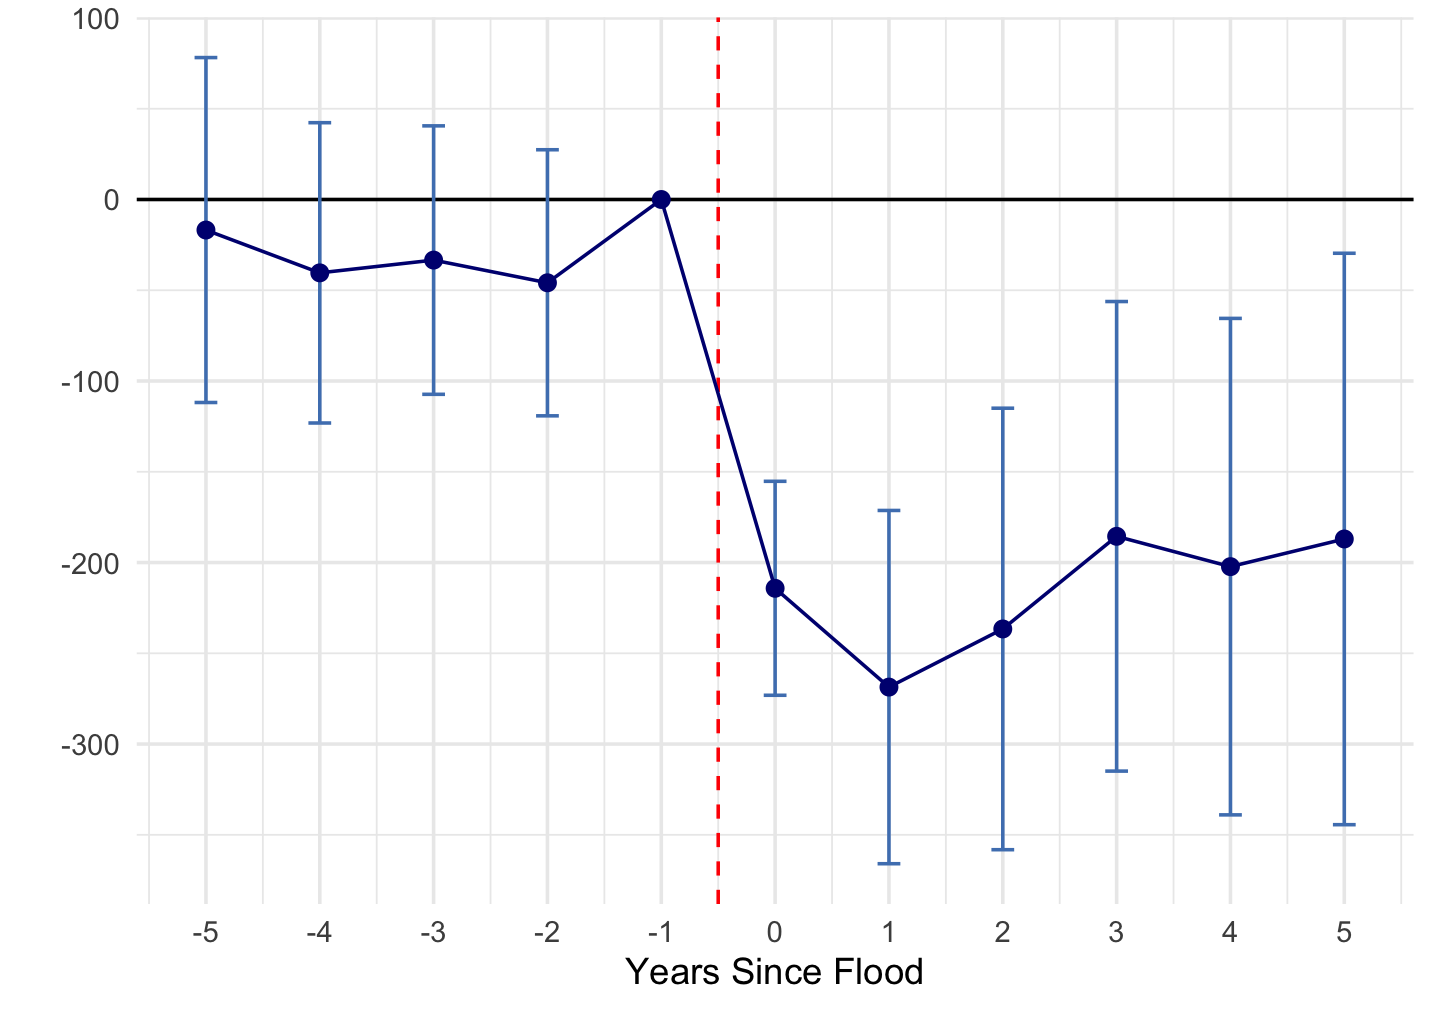
\includegraphics[width=\linewidth]{figures/Results/Analysis_Firms/AVGWAGE_3112_weighted.png}
    \subcaption{\textbf{Average wage at 31.12}}
    \label{fig:wage3112_firm}
  \end{subfigure}
  \hfill
  \begin{subfigure}[t]{0.49\textwidth}
    \centering
    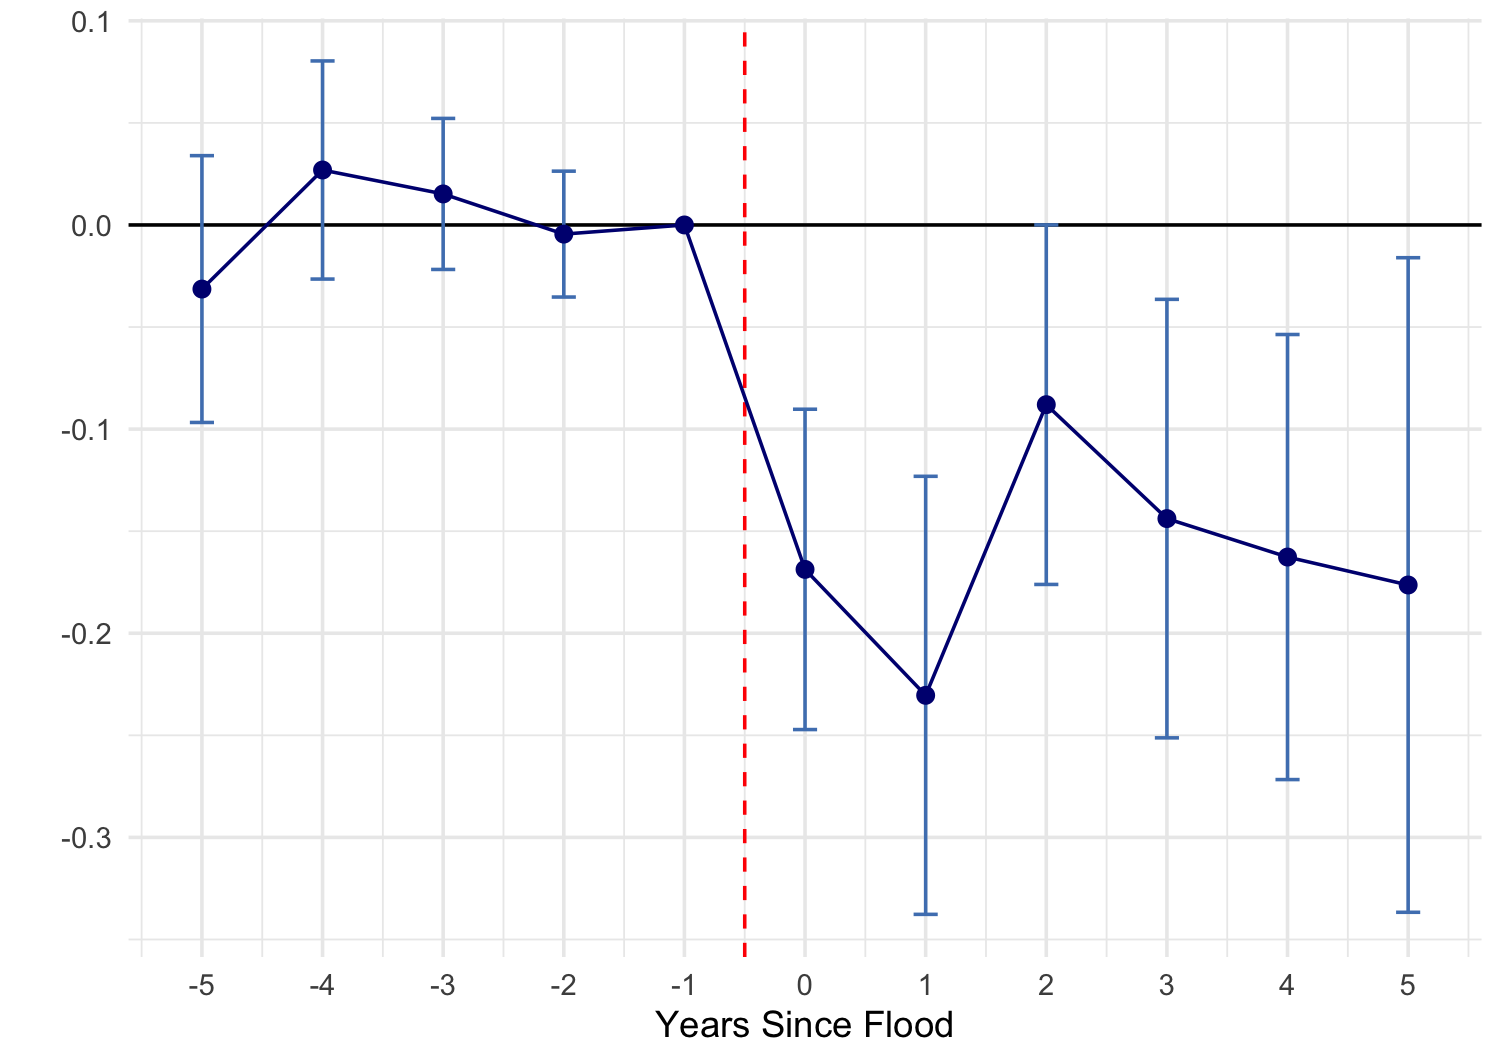
\includegraphics[width=\linewidth]{figures/Results/Analysis_Firms/EFF_3112_weighted.png}
    \subcaption{\textbf{Headcount at 31.12}}
    \label{fig:eff3112_firm}
  \end{subfigure}

  % Second row
  \begin{subfigure}[t]{0.503\textwidth}
    \centering
    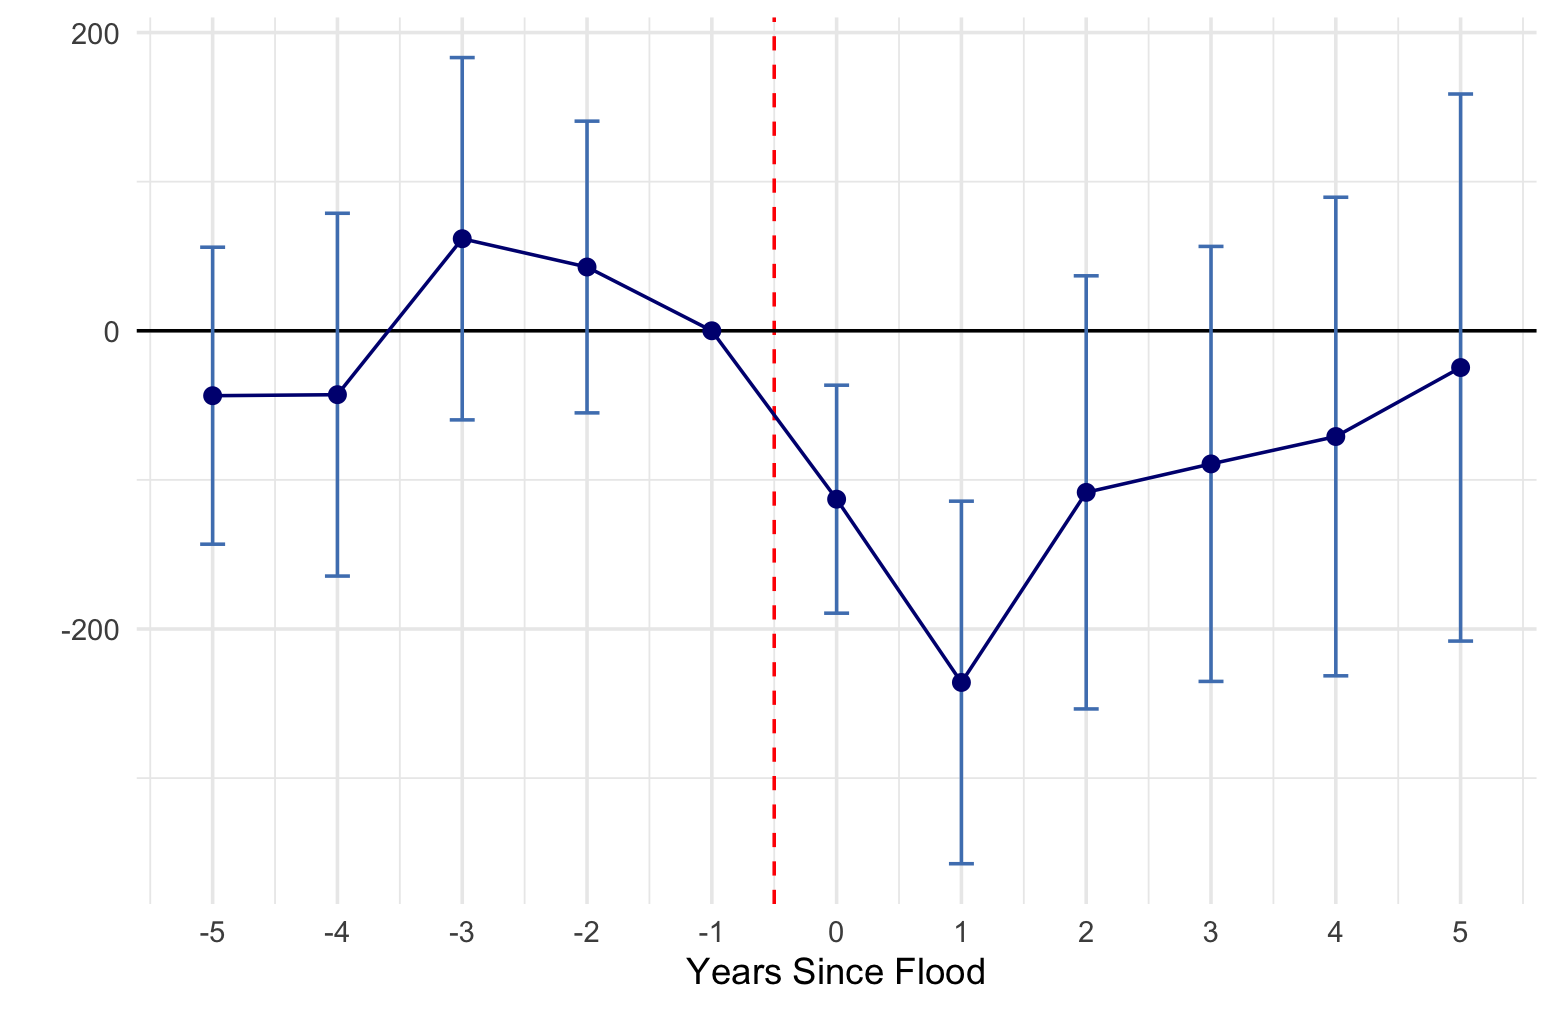
\includegraphics[width=\linewidth]{figures/Results/Analysis_Firms/AVGWAGE yearly.png}
    \subcaption{\textbf{Average Wage Yearly}}
    \label{fig:avg_wage_firm}
  \end{subfigure}
  \hfill
  \begin{subfigure}[t]{0.49\textwidth}
    \centering
    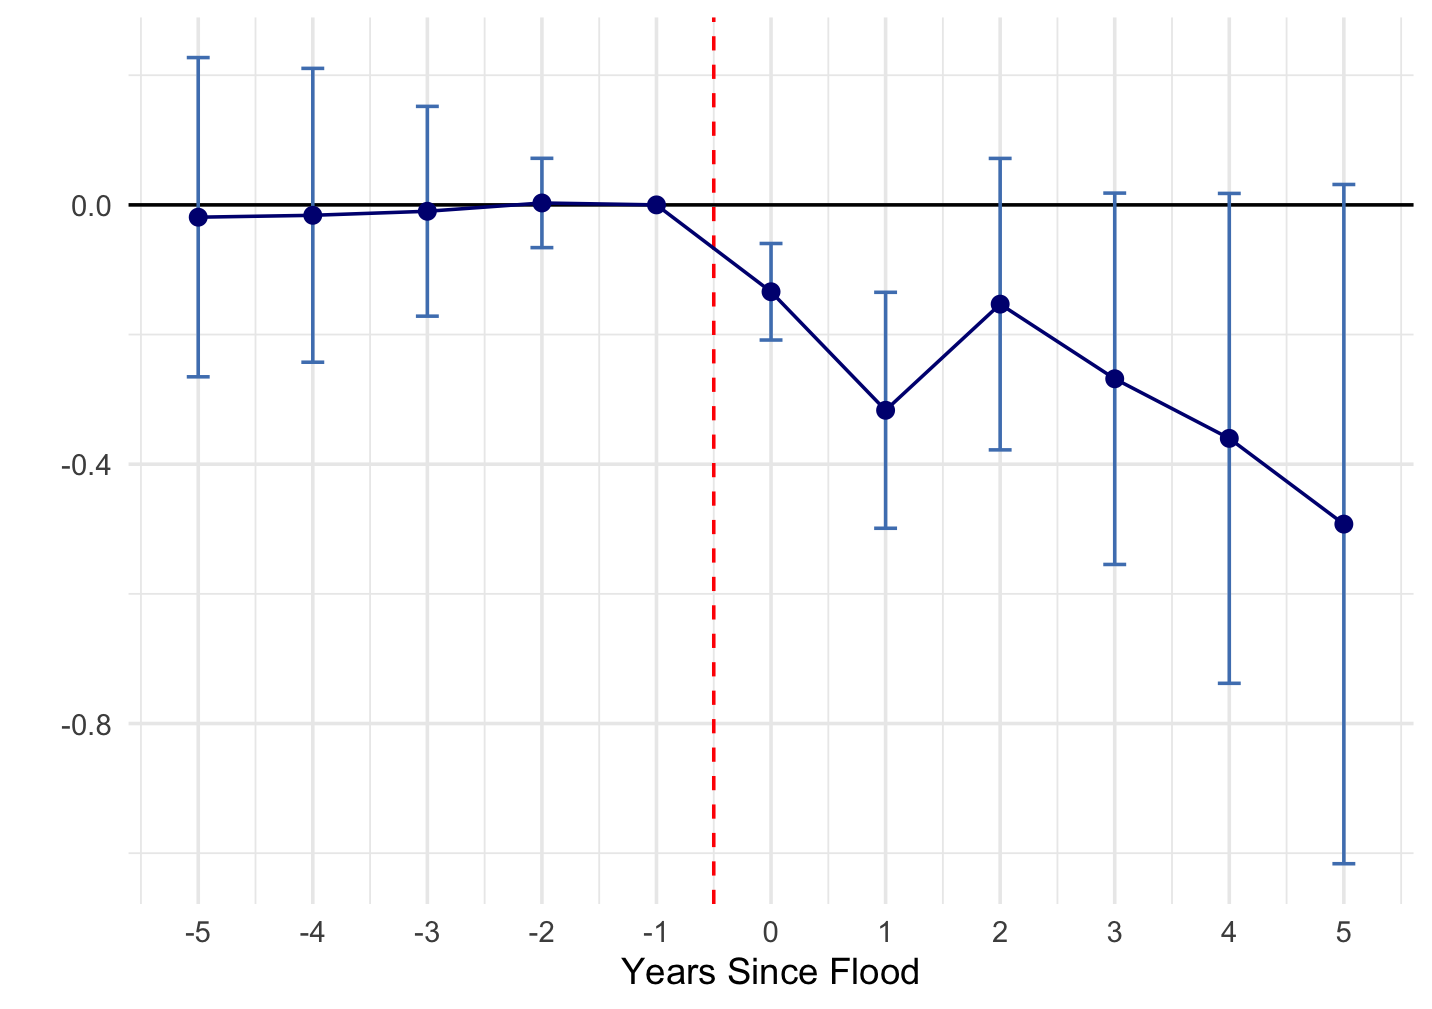
\includegraphics[width=\linewidth]{figures/Results/Analysis_Firms/EFF_ET_MOYEN_weighted.png}
    \subcaption{\textbf{Average Headcount Yearly}}
    \label{fig:avg_eff_firm}
  \end{subfigure}
  
  %\caption*{\textit{Note:} thee fixed effects,,.. the table with pooled estimates is shown in Table..}

  
\end{figure}

%%%%%%%%%%%%%%%%%%%%%%%%%%%%%%%%%%%%%%%%%%%%%%%%%%%%%%%%%
%%%%%%%%%%%%%%%%%%%%%%%%%%%%%%%%%%%%%%%%%%%%%%%%%%%%%%%%%




\begin{table}[!htbp]
\centering
\caption{\textbf{Table \ref{tab:lpdid_pooled}}: \textsc{Main LP-DiD Estimates at Establishment Level}}
\label{tab:lpdid_pooled}

\resizebox{16.3cm}{!}{
\begin{tabular}{@{\extracolsep{6pt}}p{6.5cm}cccccc}
\\[-1.8ex]\hline
\hline \\[-1.8ex]
& \multicolumn{6}{c}{\textit{Dependent variable:}} \\
\cline{2-7}
\\[-1.8ex] 
& Employment 31.12 & Wages 31.12 & Temporary contracts & Employment Yearly & Hourly Wages & Total Revenue \\
&  &  &  & & & \\
\hline \\[-1.8ex]

\textbf{Post-Treatment Average Effect} \\[0.15em]
\textit{A. Full Sample} \\[0.15em]
Treated (=1) $\times$ Post (=1) 
& $-$0.151$^{***}$ & $-$233.62$^{***}$ & $-$0.0026 & $-$0.424 & $-$0.055 & 486.689 \\
& (0.063)           & (77.57)         & (0.0025)     & (0.287) & (0.033) & (263.316) \\[0.75em]

\textit{B. By strata} \\[0.15em]
Mono-establishment (=1) 
& $-$0.022 & $-$524.13$^{***}$ & $-$0.0052 & $-$0.0070 & $-$0.170$^{**}$ & $-$15.388 \\
& (0.012)  & (127.62)          & (0.0047)  & (0.023)   & (0.079)         & (20.013) \\[0.25em]

Litorale (=1) 
& $-$0.134$^{*}$ & $-$114.26 & $-$0.0130$^{**}$ & $-$0.072 & 0.077 & 393.69 \\
& (0.180)        & (191.26)  & (0.0059)         & (0.347)  & (0.076)  & (448.64) \\[0.25em]

Mono-estab. (=1) $\times$ Litorale (=1) 
&   $-$0.031     &  $-$681.695$^{**}$  &  $-$0.038$^{**}$  &  $-$0.021     &   0.119     & $-$29.77 \\
&    (0.043)    &   (288.359)     &      ($-$0.0066)     &   (0.051)     &  (0.144)      & (19.13) \\[0.5em]

\hline \\[-1.8ex]
Total observations         & 6.82M & 6.82M & 6.82M & 6.82M & 6.82M & 6.82M \\
\textit{Fixed effects}     &       &       &       &       &       & \\
Year                       & Yes   & Yes   & Yes   & Yes   & Yes   & Yes \\
Commune                    & Yes   & Yes   & Yes   & Yes   & Yes   & Yes \\
Flood risk group $\times$ Section $\times$ Year 
                          & Yes   & Yes   & Yes   & Yes   & Yes   & Yes \\
Clustered SEs at establishment   
                          & Yes   & Yes   & Yes   & Yes   & Yes   & Yes \\

\hline
\hline \\[-1.8ex]
\multicolumn{7}{p{23cm}}{\textit{Notes:} Each column reports pooled Local Projection DiD coefficients for the post-treatment period (mean of event times $k = 0$ to $5$). Robust standard errors clustered at the establishment level (\texttt{SIRET}) in parentheses. $^{*}p<0.10$; $^{**}p<0.05$; $^{***}p<0.01$.}
\end{tabular}}
\end{table}




\\
\\
\vspace{\baselineskip}

The subsample regression results indicate that the negative impact of flooding on firm wages is more pronounced for firms with a single establishment. This is consistent with the notion that multi-establishment firms can reallocate activity across locations and thereby cushion the effects of local shocks, whereas mono-establishment firms lack this adjustment margin and are thus more vulnerable. Beyond this dimension, it would be interesting to examine the role of tangible asset intensity, since physical capital such as plants, equipment, and warehouses is particularly susceptible to flood damage.

%Firms located in cities with low government quality, indicating that poor public choices and inefficient/incompetent city management can exacerbate the negative impact of flooding? Other interesting strata would be: urban, 

%Check for france, e.g., the Amount of municipal "green" investments to fedine "green communes, Then variables such as litorale, urban, income category, disburment of “fonds Barnier” in France;  as well as the Fond Vert. firm size can be used! FIrms with more intangible assets! only manufacturing so "active etablussment", like \cite{erda2024disasters}. Our subsample regression results reveal that the negative impact of flooding on firm wages and labour demand is more pronounced for firms with single stablishemnts. OR i could check with more intensive tangible asset investment, likely because tangible capital assets such as plants, equipment and warehouses can suffer significant damages due to flooding. \\we find that the negative impact of flooding on firm performance is significantly greater for firms facing tight financial constraints.\\ \href{https://pmc.ncbi.nlm.nih.gov/articles/PMC9278787/#pone.0271309.ref001}{source}


Finally, there is potential attrition at the extensive margin: plants that exit remain recorded in the DADS with zero workers, but may disappear entirely from the revenue panel. This can generate survivorship bias that dampens the estimated effects on sales or profits unless exits are explicitly coded as zero. Survival analyses, which are not undertaken in this paper, can be found in \cite{erda2024disasters}, \cite{fatica2024floods}, and \cite{clo2024impact}. A further limitation concerns the treatment definition. Commune-level flood dummies may adequately capture labor market disruptions, but they are likely to attenuate estimated effects on output when only part of an industrial zone is affected. Future specifications could address this by interacting the treatment with flood depth or with the share of commune area inundated, thereby capturing variation in exposure intensity more accurately.


\section{Sectoral heterogeneity in the impact of flooding}

To understand how the effects of flooding vary across the economy, I explore heterogeneity along a key dimension: the sector of activity. Figure~\ref{fig:firms_results_heter} displays event study estimates of average wage and headcount at the end of year ($31.12$), disaggregated by sector. Several patterns emerge.

\begin{figure}[htbp]
\centering
\caption{\textbf{Figure \ref{fig:firms_results_heter}:} Sectoral heterogeneity in the impact of flooding}
\label{fig:firms_results_heter}
\begin{subfigure}[t]{0.49\textwidth}
\centering
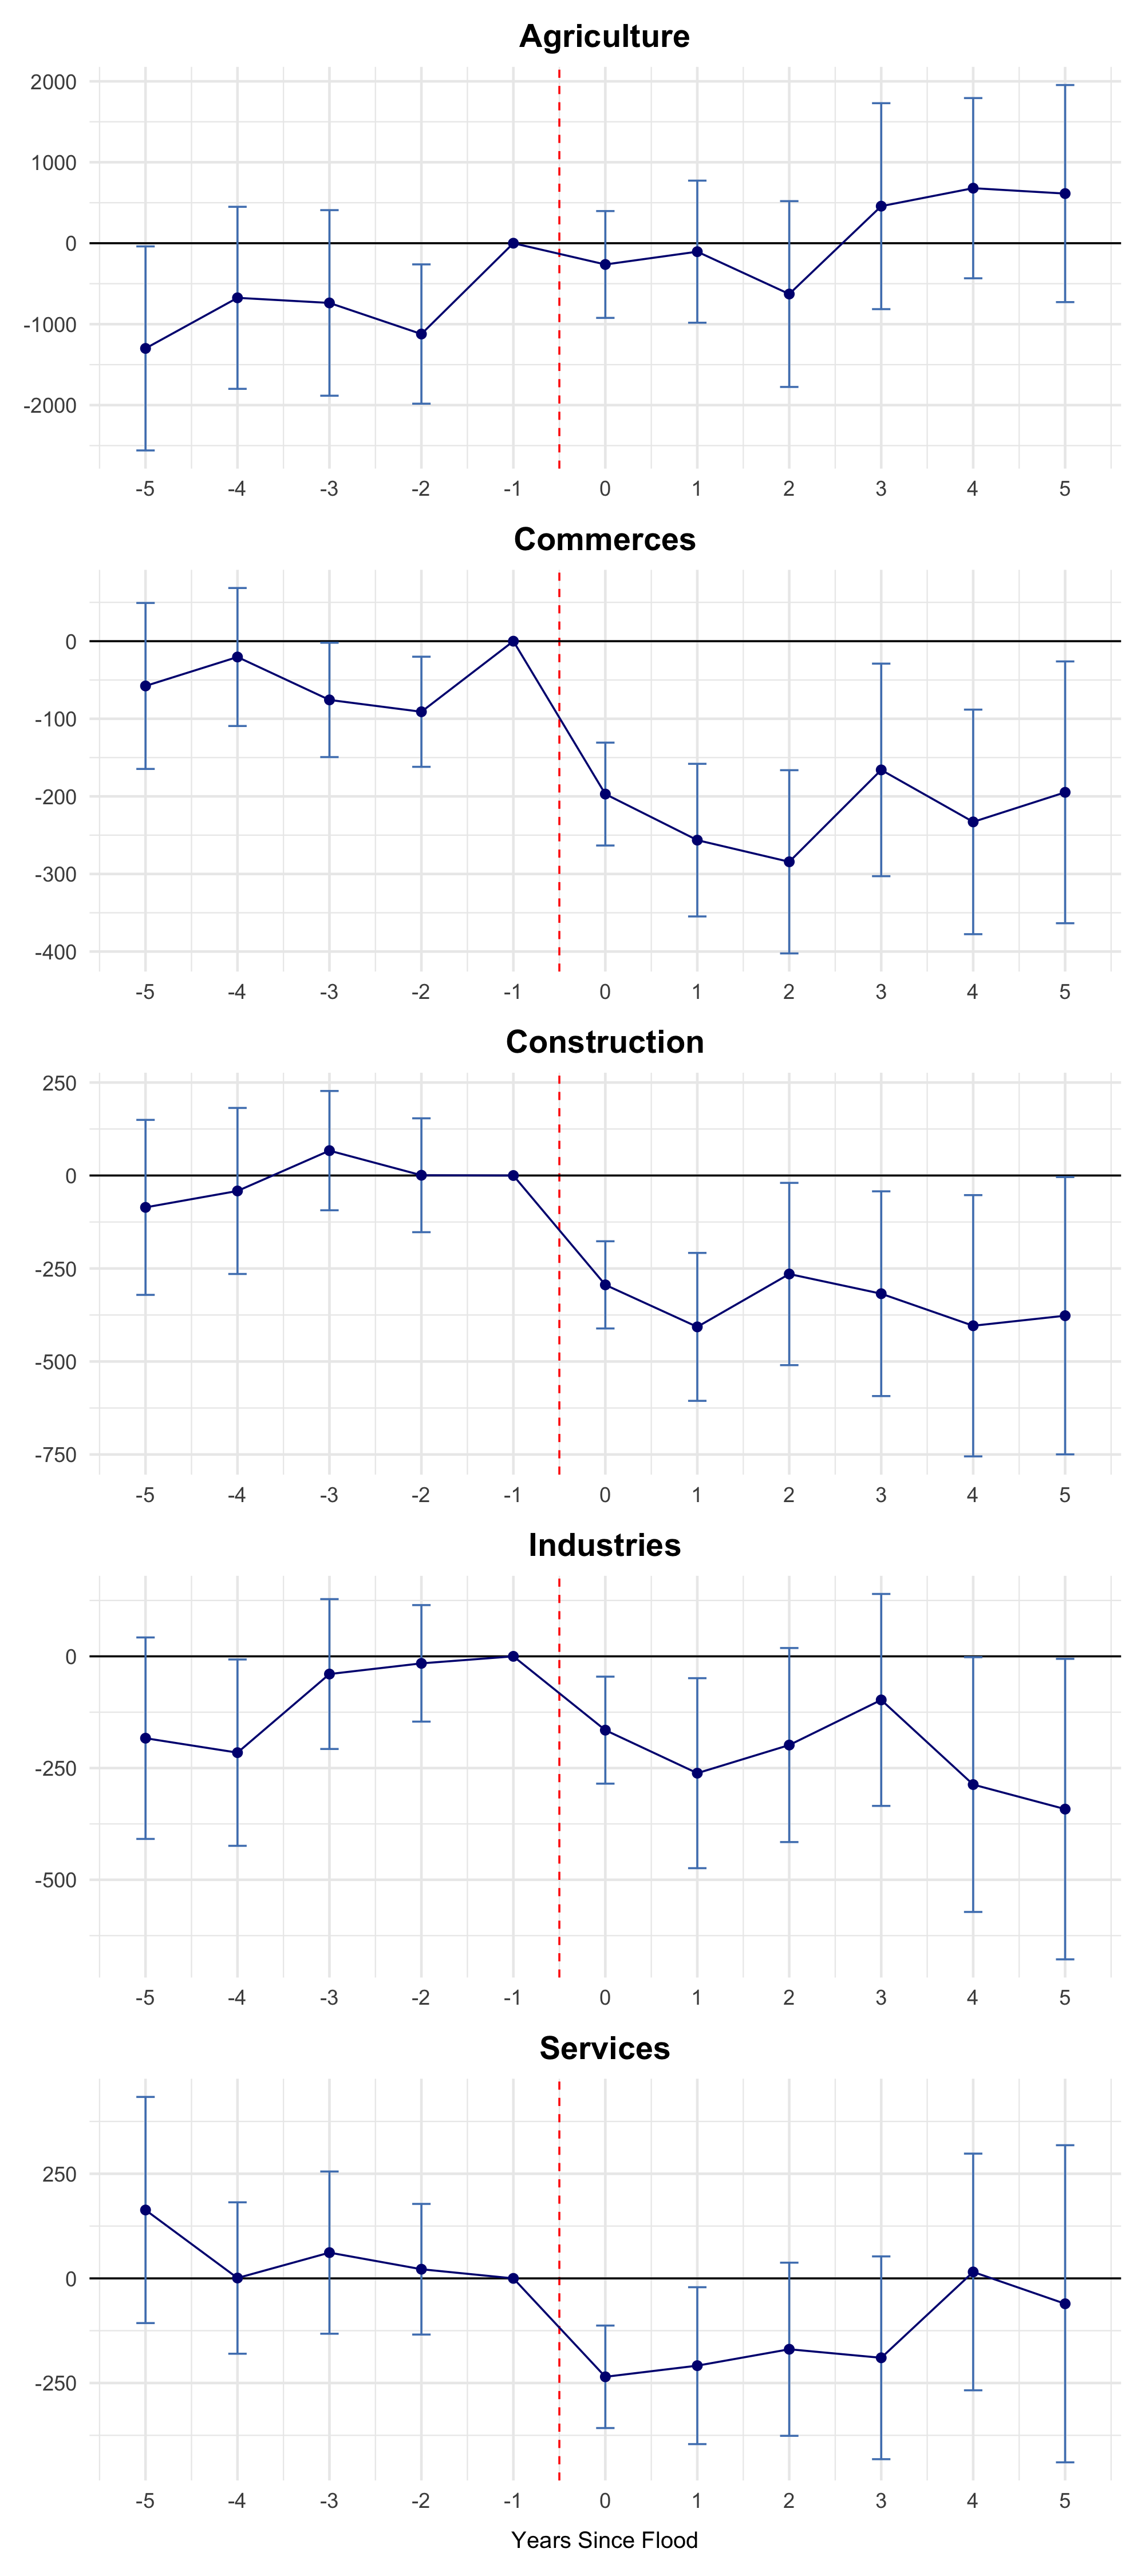
\includegraphics[width=\linewidth]{figures/Results/Analysis_Firms/AVGWAGE_3112_Sectors.png}
\subcaption{\textbf{Average wage at 31.12}}
\label{fig:avg_wage_firm_heter}
\end{subfigure}
\hspace{0.02cm}
\begin{subfigure}[t]{0.49\textwidth}
\centering
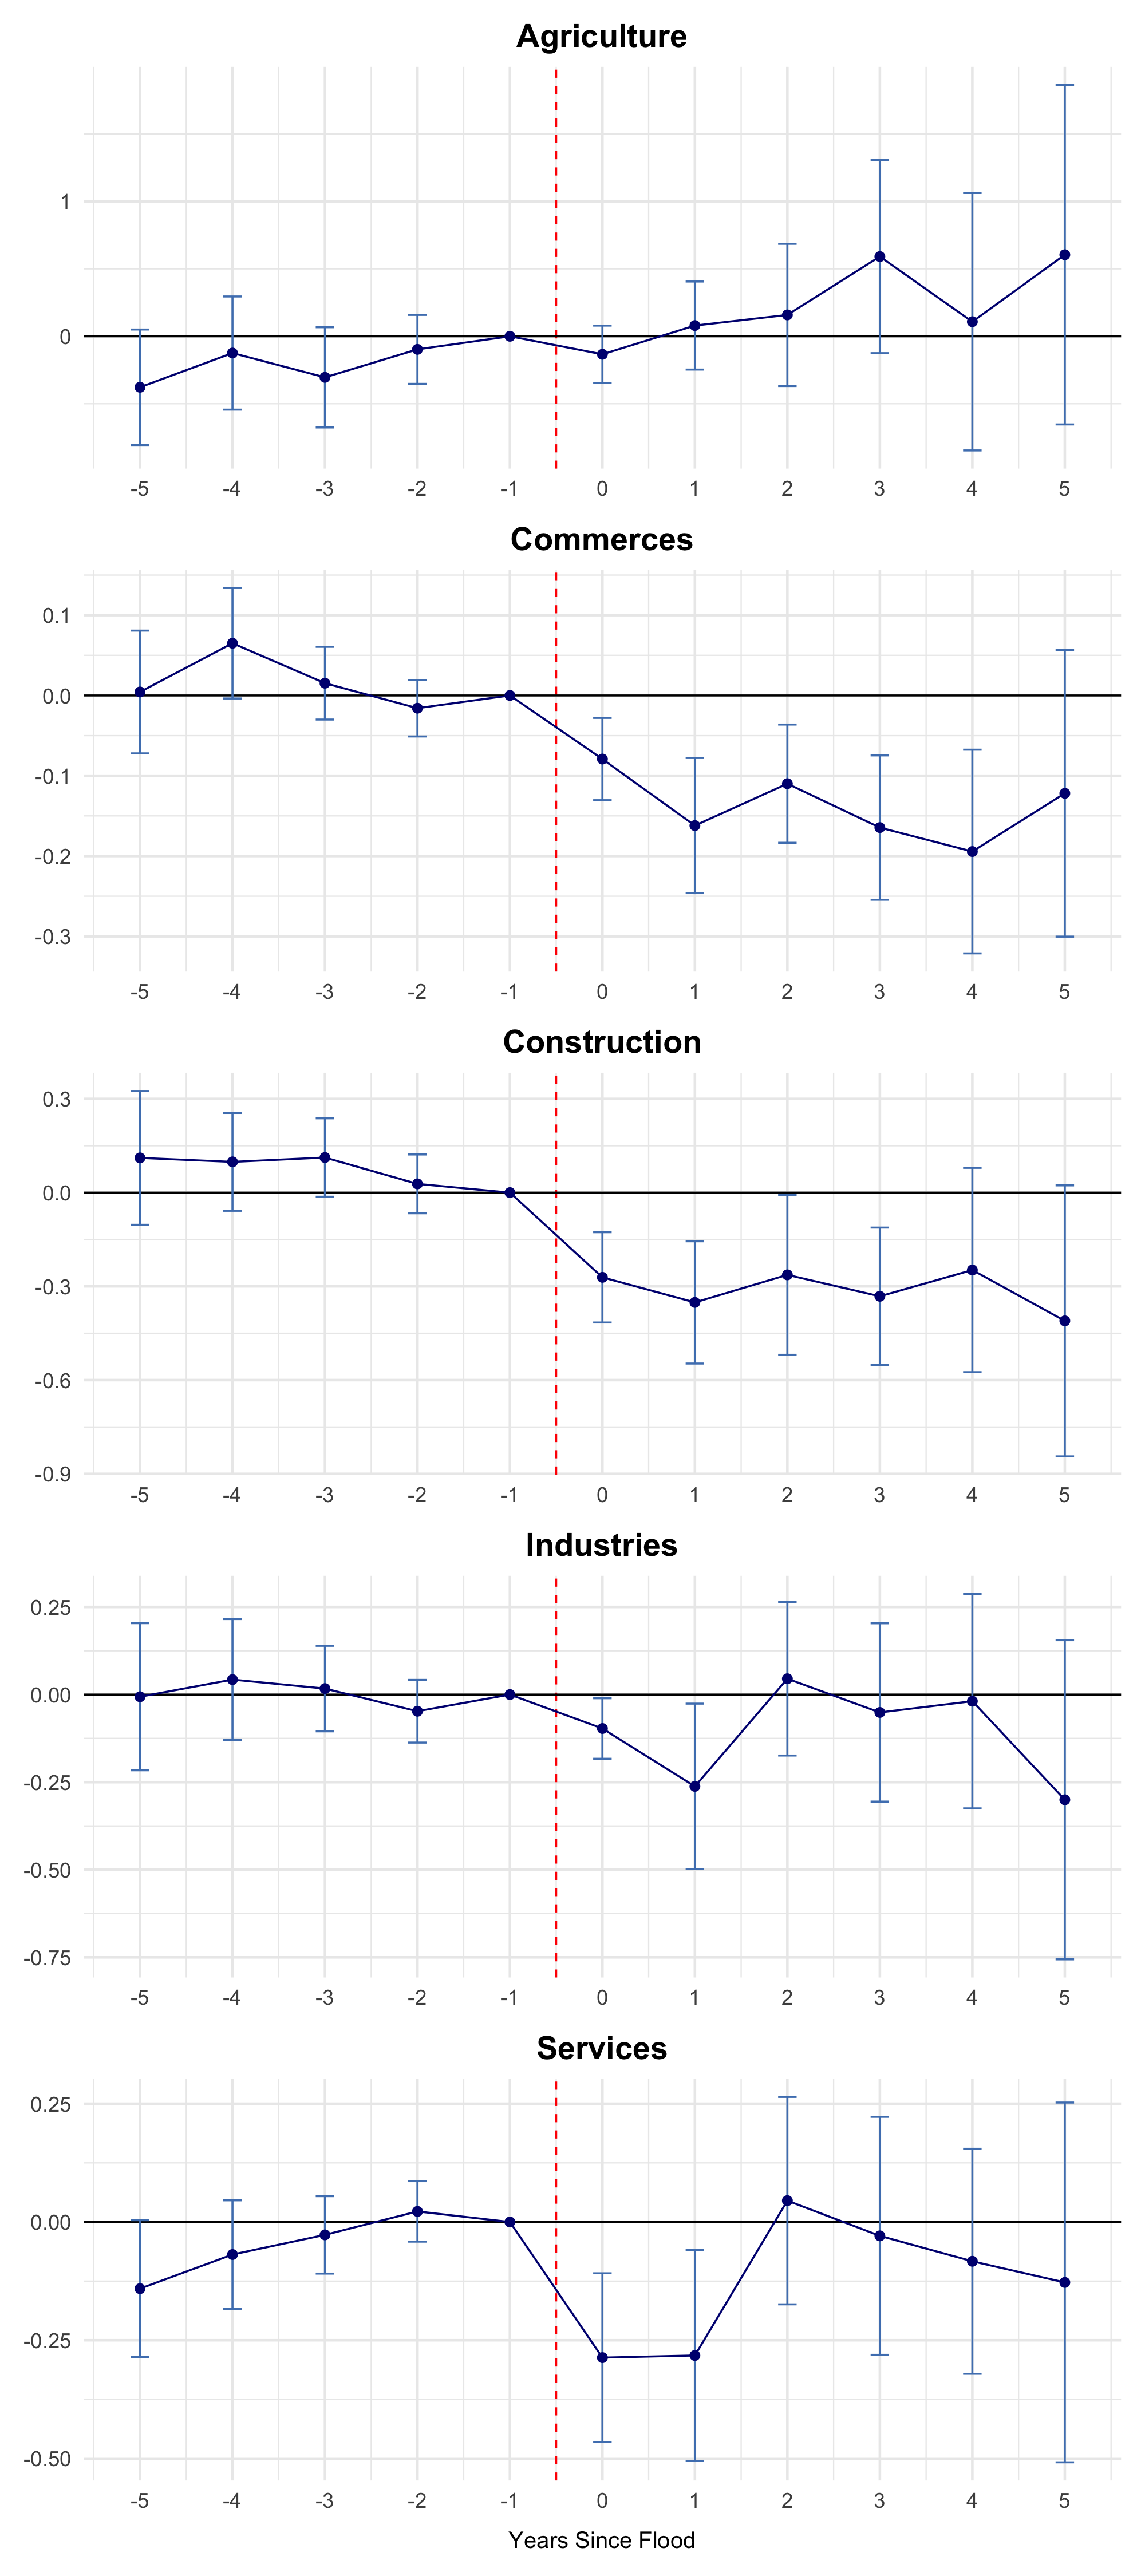
\includegraphics[width=\linewidth]{figures/Results/Analysis_Firms/EFF_3112_Sectors.png}
\subcaption{\textbf{Headcount at 31.12}}
\label{fig:eff3112_firm_heter}
\end{subfigure}

\vspace{0.8em}
\end{figure}


First, the parallel-trends assumption appears to hold across all sector panels: coefficients on the leads ($k = -5$ to $k = -2$) are statistically indistinguishable from zero, supporting the identifying assumption of the LP-DiD design. Turning to the post-flood dynamics, Panels (a) and (b) show that all sectors except agriculture experience some decline in average wages and employment, though the intensity and persistence vary considerably.

In commerce, employment drops sharply—by about 20\% in the first year after a flood ($k=1$)—and losses persist through $k=5$. Construction suffers the most severe and prolonged effects, with employment falling by up to 30\% around $k=3$, despite the potential for increased reconstruction demand. These results indicate that both sectors are especially vulnerable to flooding, likely due to their reliance on physical storefronts, infrastructure, and on-site activity. Services also show a persistent decline, though of a more moderate scale (10–15\%). This suggests that local service providers face sustained challenges after floods, stemming from demand shifts, commuting disruptions, or damage to premises, and they may be unable to reorganize production flexibly, as argued by \cite{indaco2021hurricanes}.

By contrast, the industrial sector shows little to no systematic response: coefficients fluctuate around zero and remain statistically insignificant, pointing to greater flood resilience, possibly due to larger capital buffers, insurance coverage, or geographic insulation from flood-prone areas. Similarly, the agricultural sector exhibits high variance but no consistent directional effect, with noisy estimates centered around zero. This pattern may reflect strong adaptation mechanisms in farming or substantial heterogeneity within the sector.

Taken together, these results suggest that sectors relying heavily on localized retail activity, manual labor, and in-person service delivery (commerce, construction, many services) bear the brunt of flood impacts. In contrast, sectors with more fixed capital, non-localized markets, or better insurance coverage (industry, agriculture) tend to show quicker recovery or minimal disruption. Importantly, these estimates are based on unweighted regressions. If sectoral heterogeneity shrinks or disappears when using inverse probability weights, this would imply that part of the observed variation reflects selection or compositional differences rather than true underlying disparities in vulnerability. Looking ahead, it would be interesting to examine whether floods also trigger climate transition-type reallocations across industries. Input–output data and information on downstream supplier relationships could help uncover whether flood shocks accelerate structural shifts in production networks.

%%%%%%%%%%%%%%%%%%%%%%%%%%%%%%%%%%%%%%%%%%%%%%%%%%%%%%%%%%%
\section{Commune level analysis}
As aggregate dynamics can differ from individual dynamics, I also run a commune-level analysis, which is the level at which treatment is administratively assigned. It could be interesting in future work to extend this to Local Labour Market (LLM) zones, by interacting commuting zones and APE codes and weighting establishment outcomes by their labor shares in the LLM.
At the commune level, however, the results show no strong or persistent impacts of floods on wages, employment, revenues, share capital, or profits (Figure \ref{fig:IRF_Communes}). This contrasts with the establishment-level results, where floods generated sharp short-term shocks on wages and employment. The absence of aggregate effects highlights recovery dynamics at the municipal scale, consistent with findings in the literature. For instance, \cite{leiter2009creative} document that while Austrian firms suffered severe direct damages from floods, municipal-level aggregates showed relatively rapid recovery due to insurance payouts and redistribution. Similarly, \cite{usman2024going} stress that commune-level indicators often conceal heterogeneity in the impact of extreme weather events, as losses in some establishments are compensated by resilience and adaptation elsewhere in the local economy.
% As aggregate dynamics can differ from individual dynamics, I run a commune level anaylsis, which is the level at which treatmetn is administret. It could be interesting to add to the analysis by running a Local Labour Market level analysis, by creating such zones multiplying Commuting zone and APE codes, and weighting SIRETs outcomes by their labour share in the LLM.

% I see that at commune level there is no such big impacts, this hilights aggreagte recovery dynamics as is pointed out in Leiter or at page. 6 and 28 of going NUTS! SInce no apparetn aggregate impact, they run on communes based on income of commune! I will do this!

% \textbf{Mechanisms:} This designation of flooding episode is place-based, referring to the specific municipalities affected, and primarily triggers compulsory insurance coverage for the damages sustained—it does not automatically unlock substantial public funding for infrastructure reconstruction or direct grants to households and businesses. Nevertheless, it ensures regulated insurance payouts, offering financial relief to those impacted by the floods. \cite{indaco2021hurricanes} finds similar results.


%%%%% Figure: Flood Impacts commune level
\begin{figure}[htp]
  \centering

      \caption{\textbf{Figure \ref{fig:IRF_Communes}:} Flood impacts at the commune level}
    \label{fig:IRF_Communes}
    
  % First row
  \begin{subfigure}[b]{0.33\textwidth}
    \centering
    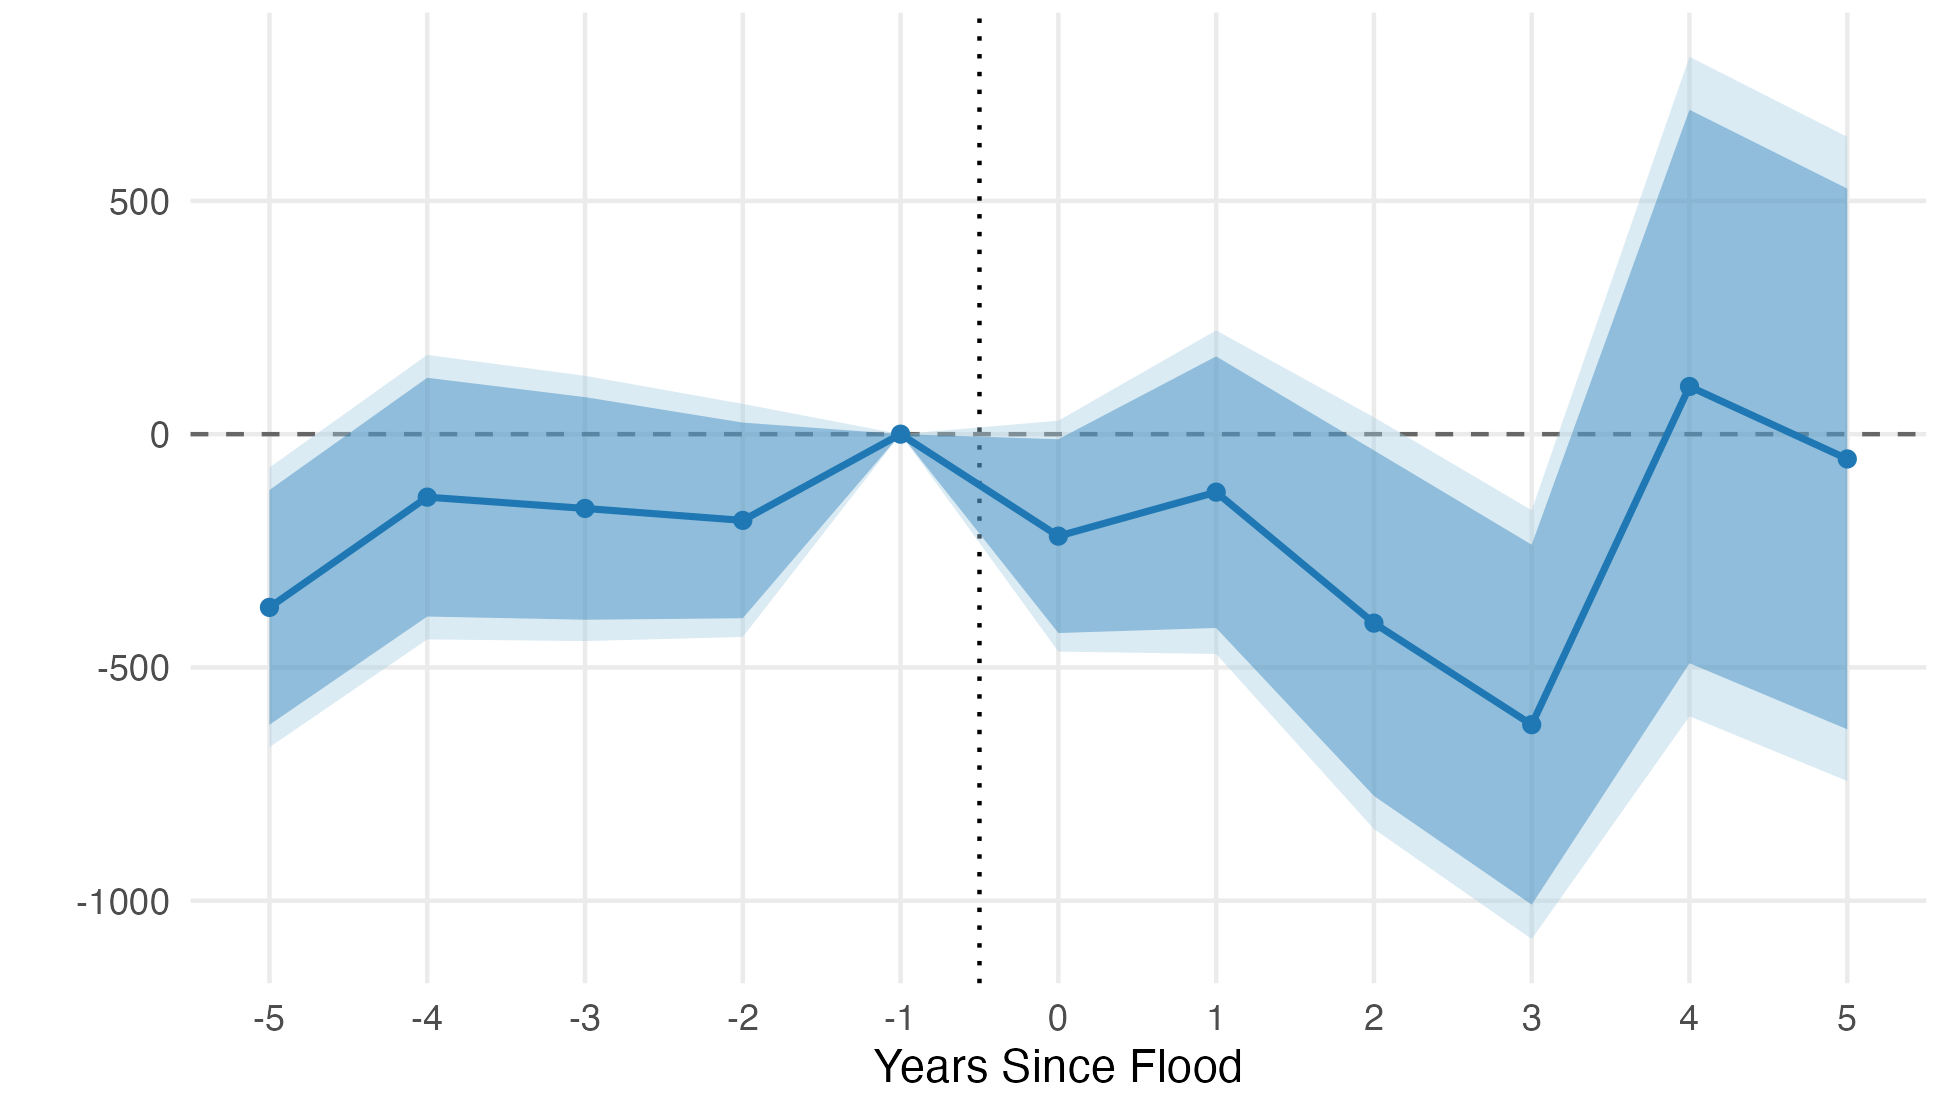
\includegraphics[width=\linewidth]{figures/Results/Analysis_Communes/IRF_AVGWAGE_3112_pooled.png}
    \subcaption{Wages at 31.12}
    \label{}
  \end{subfigure}%
  \begin{subfigure}[b]{0.33\textwidth}
    \centering
    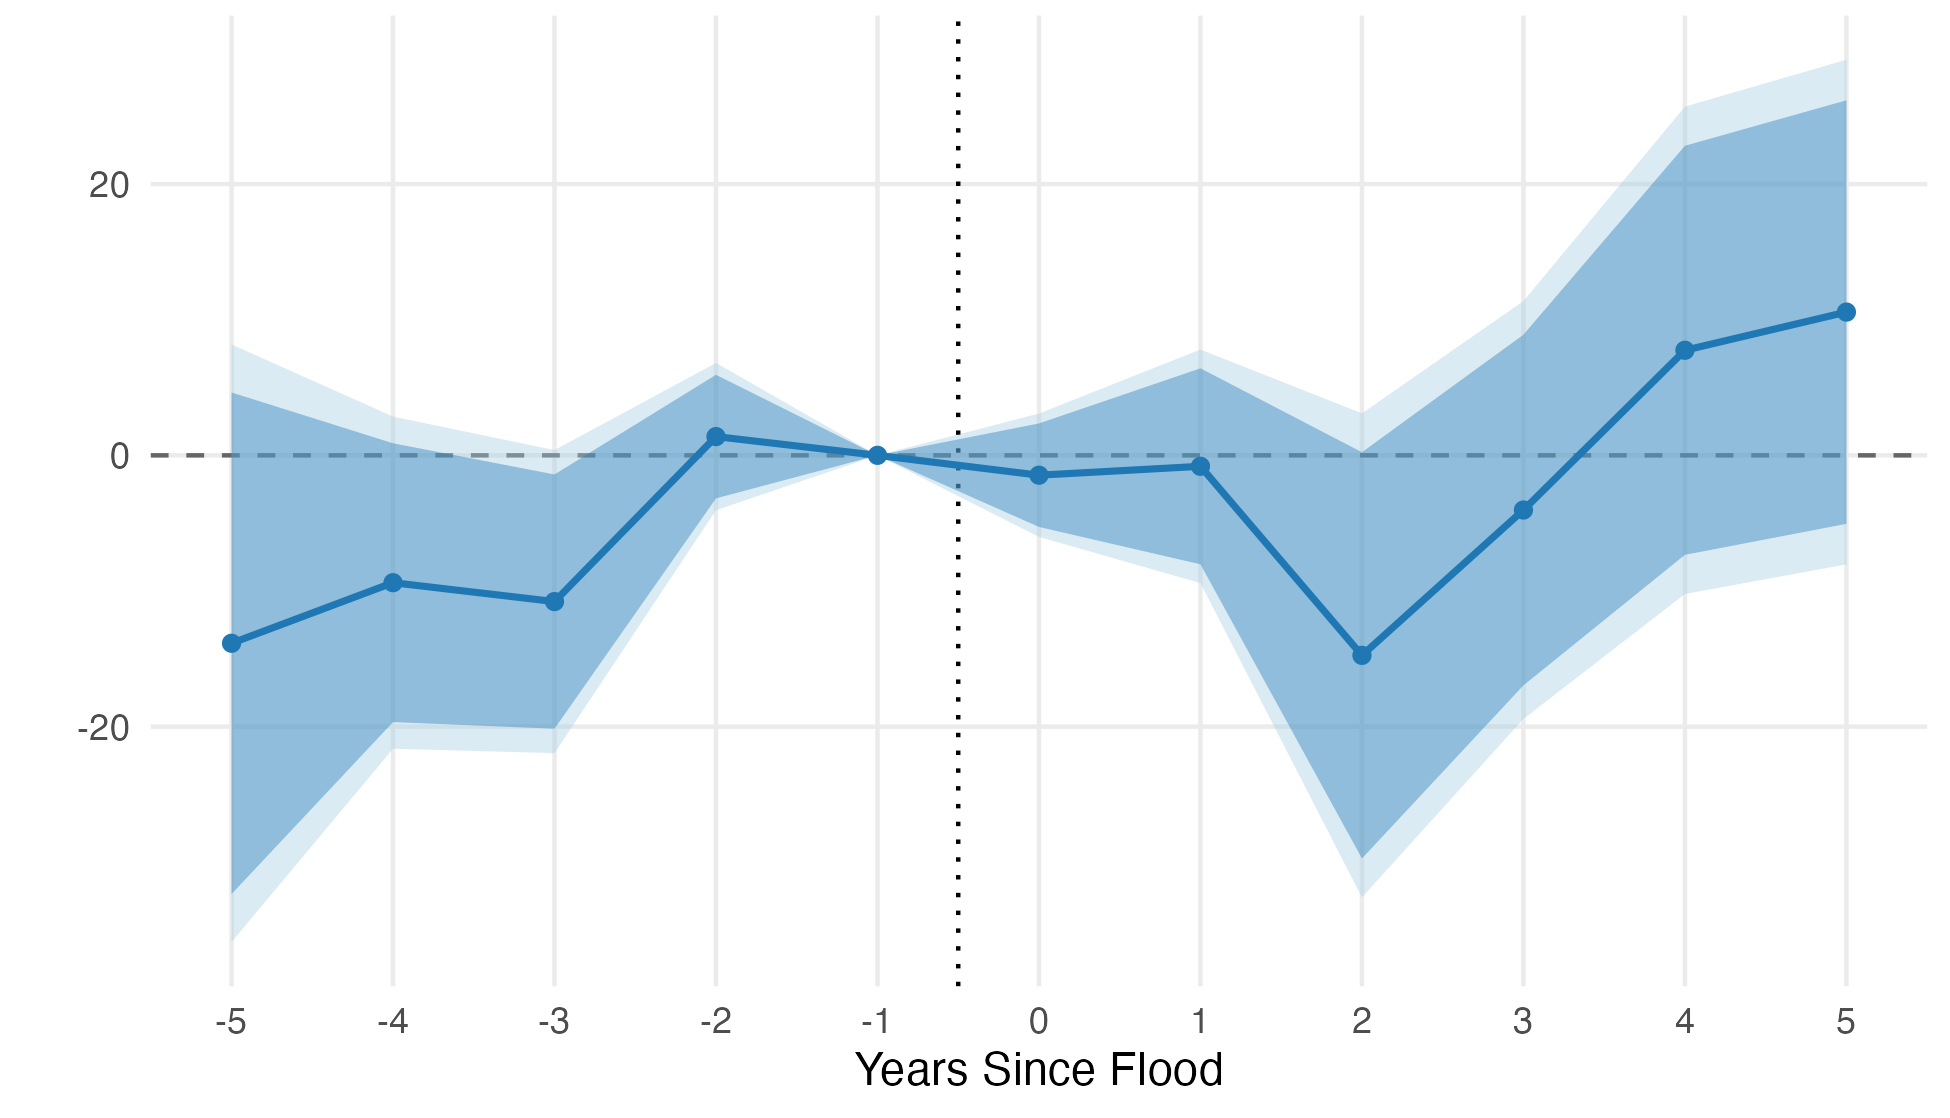
\includegraphics[width=\linewidth]{figures/Results/Analysis_Communes/IRF_EFF_3112_pooled.png}
    \subcaption{Headcount at 31.12}
    \label{fig:eff_all_commmune}
  \end{subfigure}
  \begin{subfigure}[b]{0.33\textwidth}
    \centering
    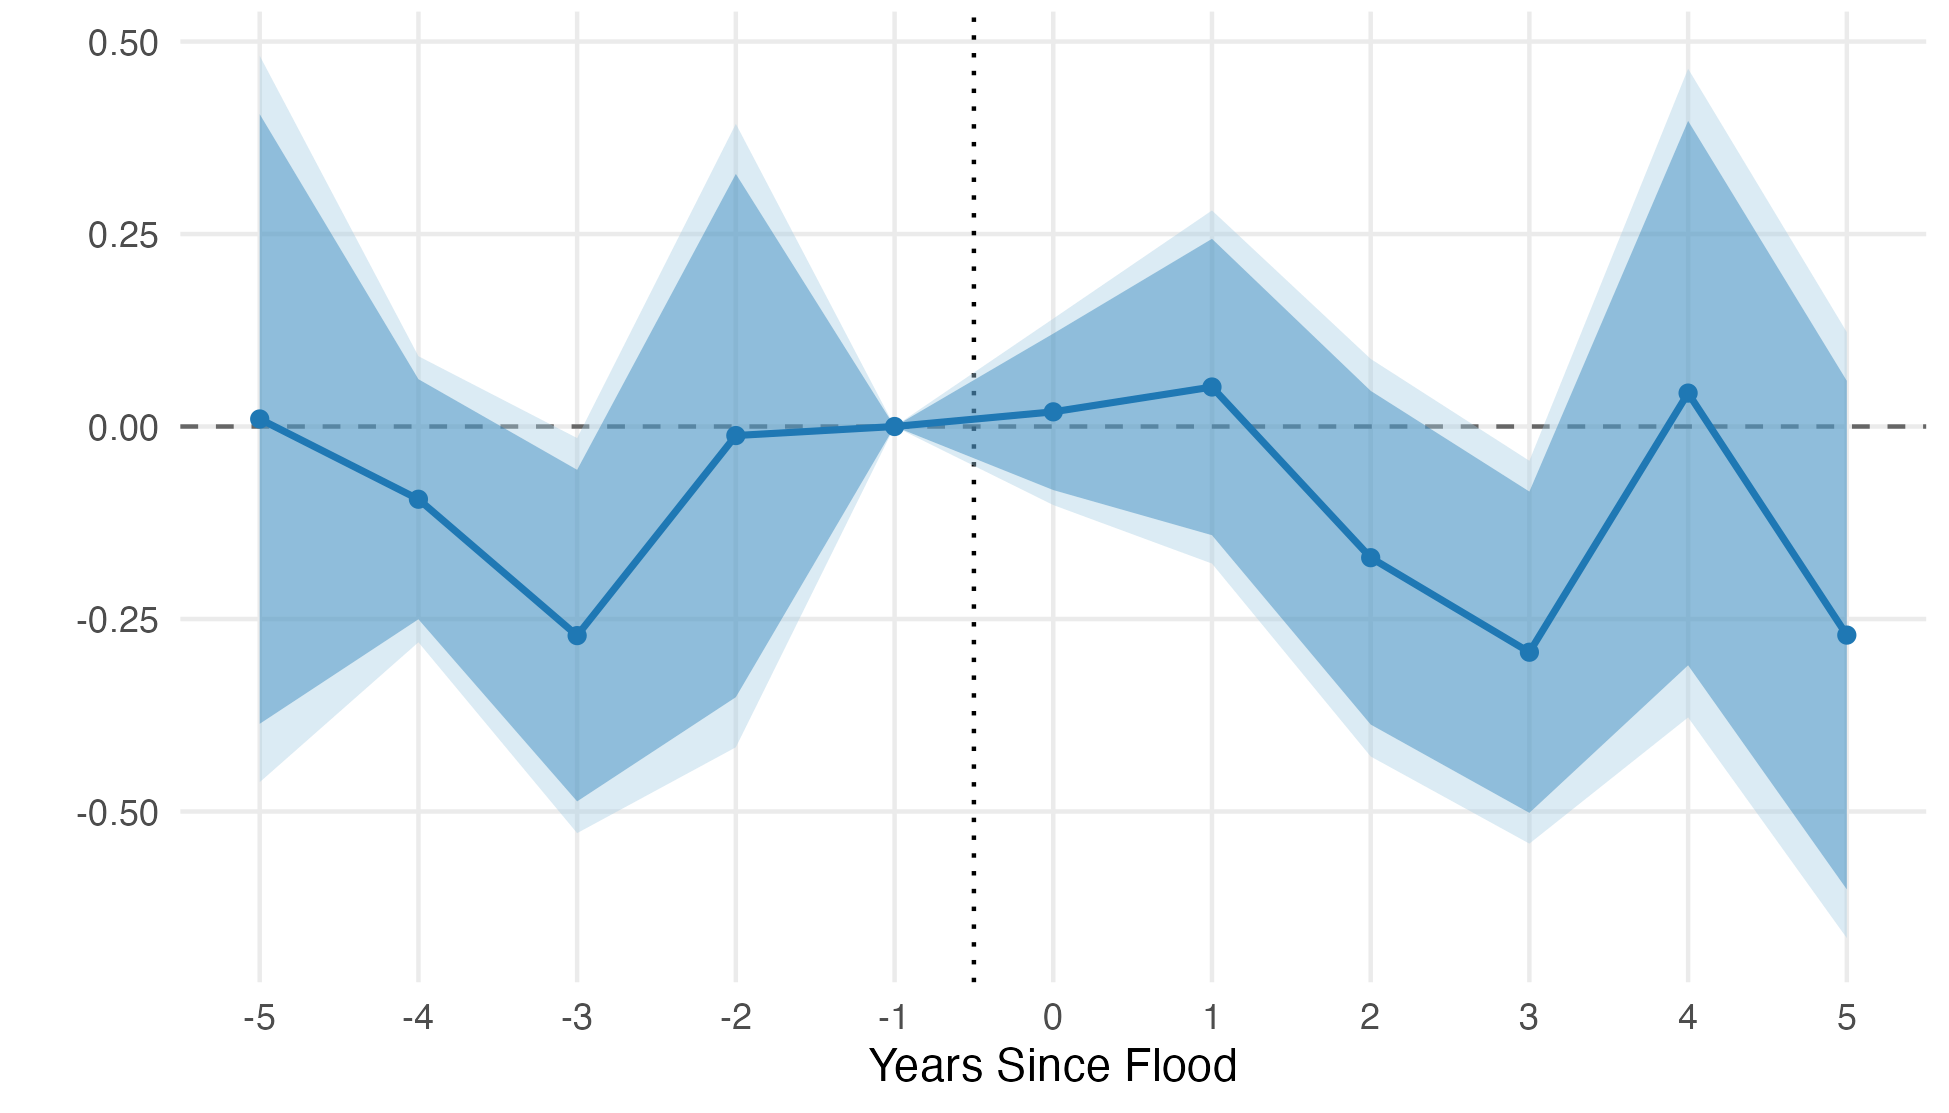
\includegraphics[width=\linewidth]{figures/Results/Analysis_Communes/IRF_HWAGE_3112_pooled.png}
    \subcaption{Hourly Wage}
    \label{}
  \end{subfigure}

 
 \vspace{0.8em}
 
    \begin{subfigure}[b]{0.33\textwidth}
    \centering
    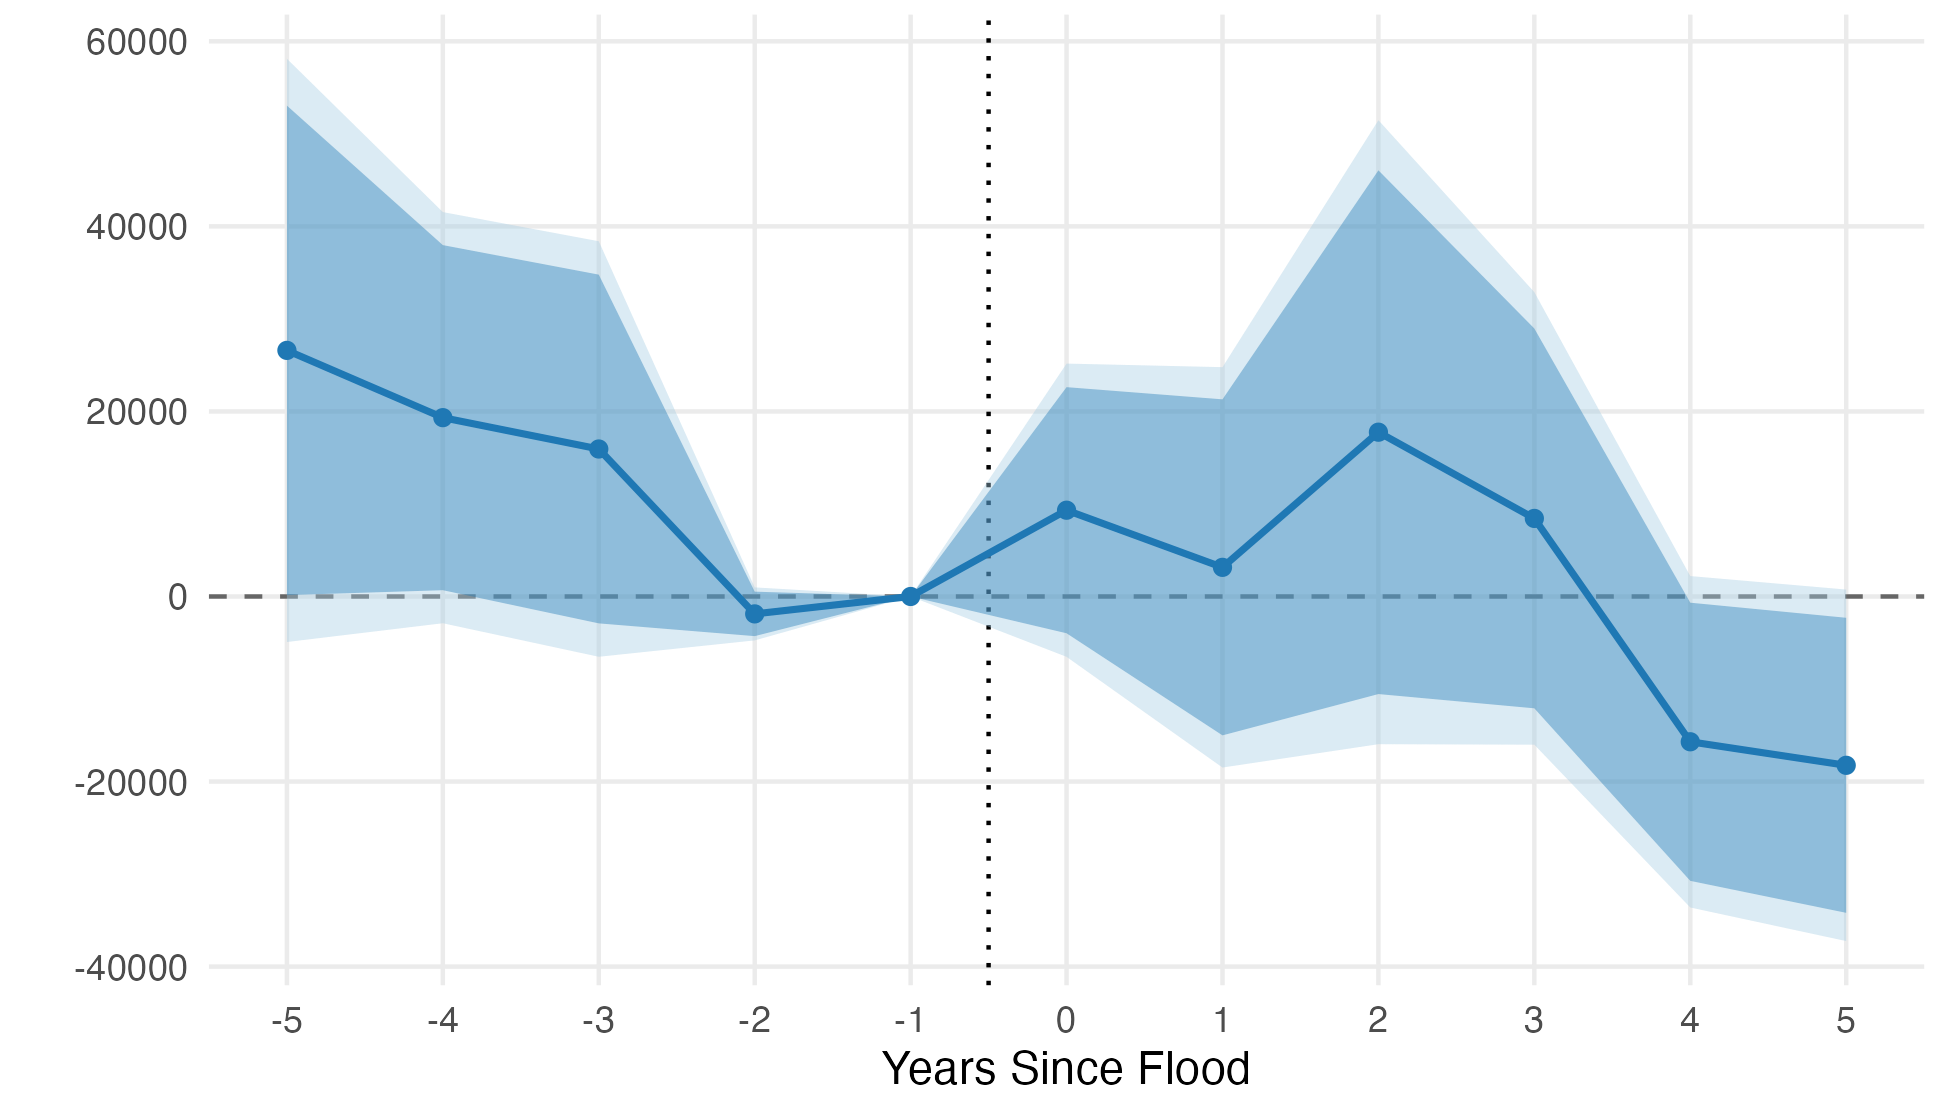
\includegraphics[width=\linewidth]{figures/Results/Analysis_Communes/IRF_redi_r310_SIRET_pooled.png}
    \subcaption{Total Revenue}
    \label{}
  \end{subfigure}
  \begin{subfigure}[b]{0.33\textwidth}
    \centering
    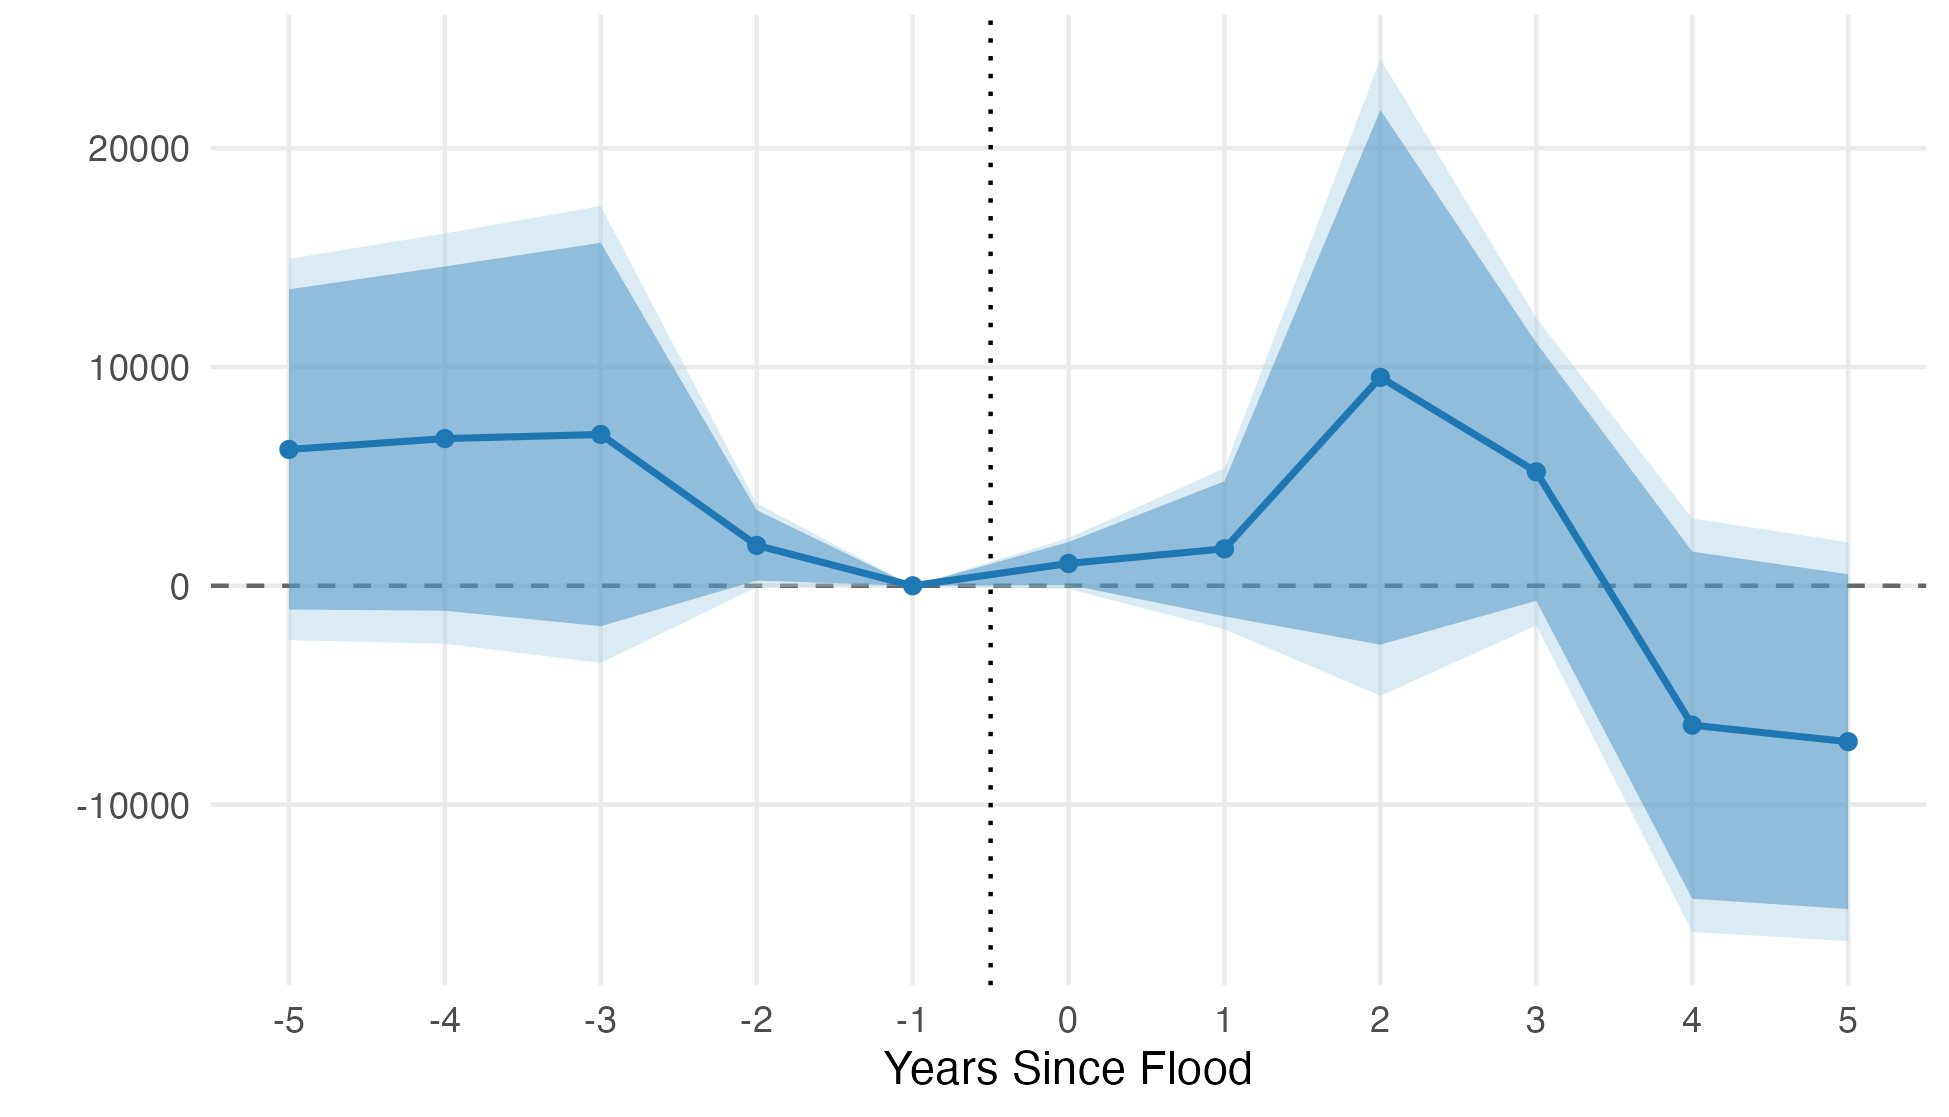
\includegraphics[width=\linewidth]{figures/Results/Analysis_Communes/IRF_CAPISOC_SIRET_pooled.png}
    \subcaption{Share capital}
    \label{}
  \end{subfigure}
  \begin{subfigure}[b]{0.32\textwidth}
    \centering
    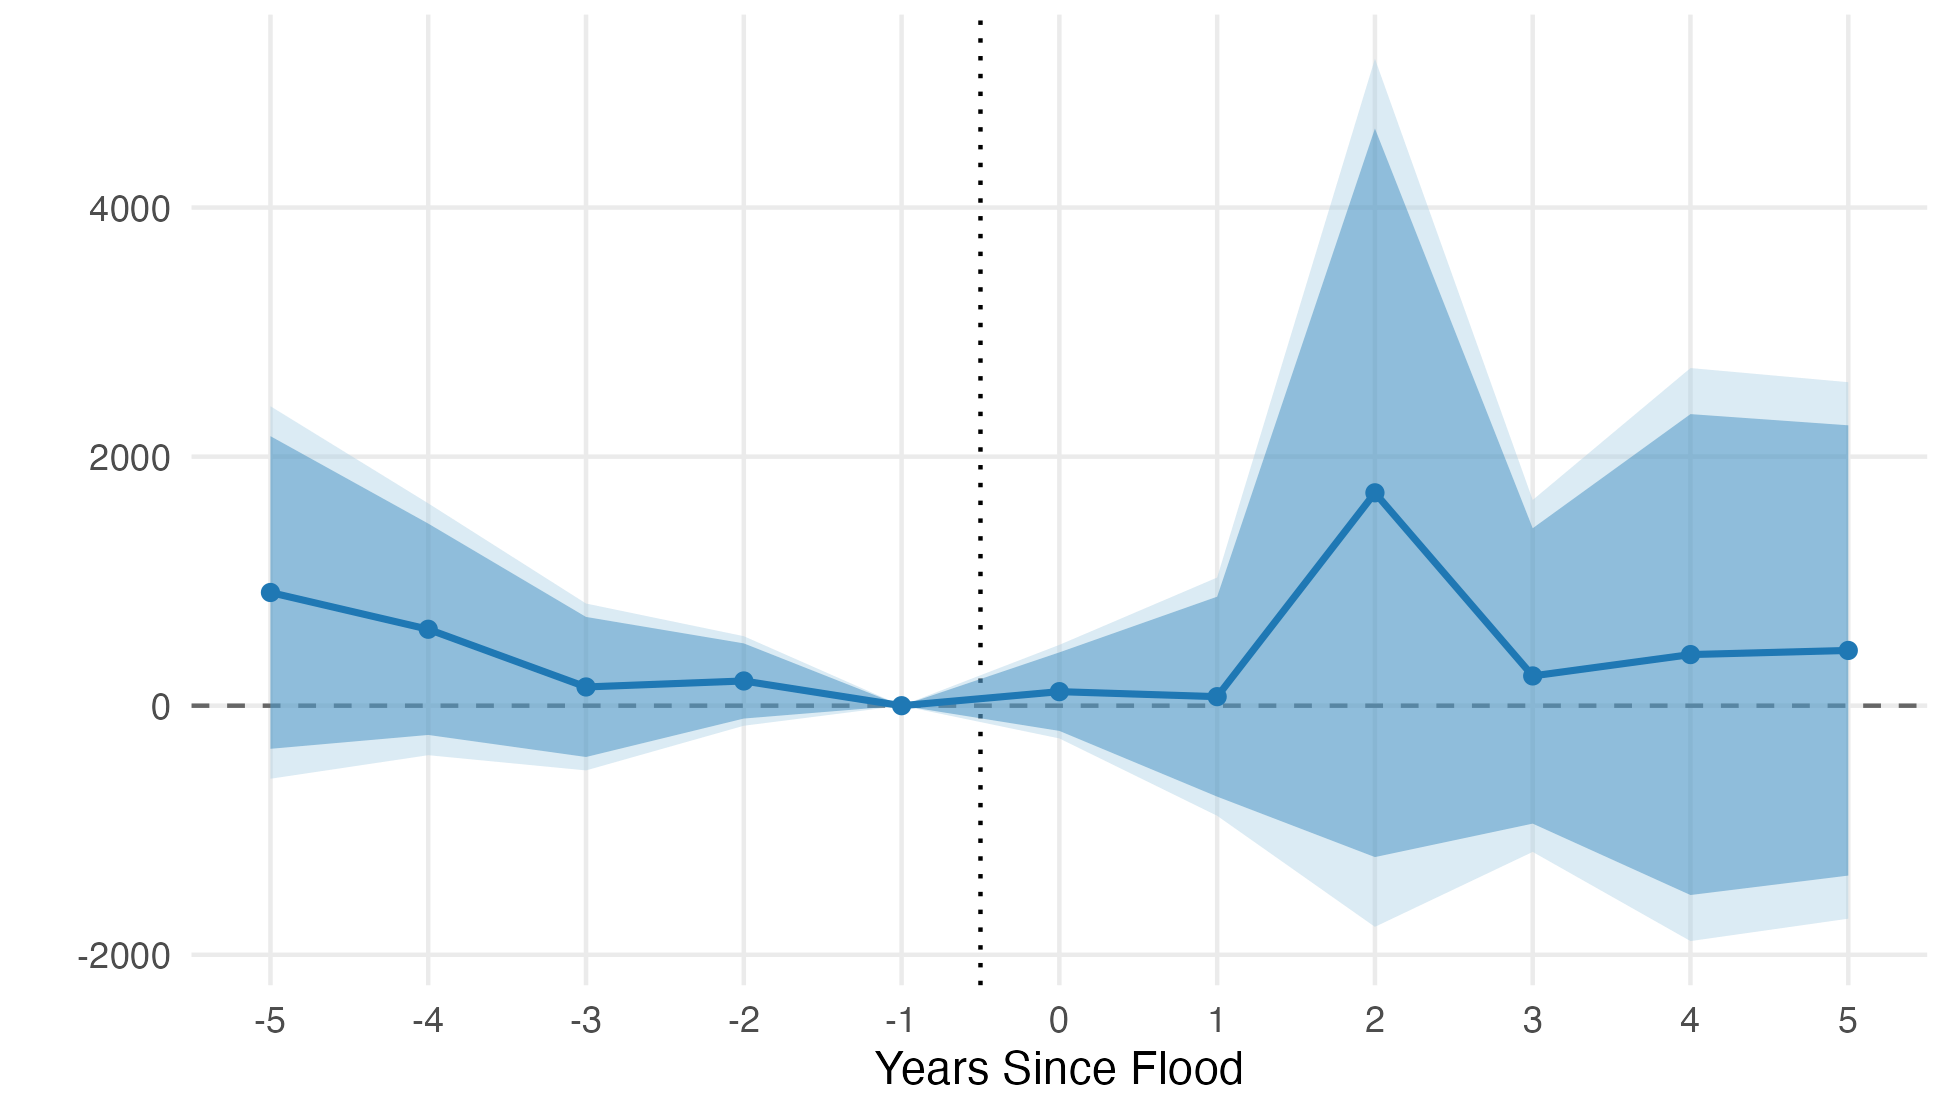
\includegraphics[width=\linewidth]{figures/Results/Analysis_Communes/IRF_b319_SIRET_pooled.png}
    \subcaption{Current profit before tax}
    \label{}
  \end{subfigure}


\end{figure}

%%%%%%%%%%%%%%%%%%%%%%%%%%%%%%%
\begin{figure}[htbp]
  \centering
  \caption{\textbf{Figure \ref{fig:IRF_litorale_comparison}:} Flood impacts by coastal exposure (litorale)}
  \label{fig:IRF_litorale_comparison}
  
    \begin{subfigure}[b]{0.45\textwidth}
    \centering
    \textbf{Litorale = 0}
  \end{subfigure}
  \hspace{1em}
  \begin{subfigure}[b]{0.45\textwidth}
    \centering
    \textbf{Litorale = 1}
  \end{subfigure}

  \vspace{0.8em}
  
  % Row 1: EFF3112
  \begin{subfigure}[b]{\textwidth}
    \centering
    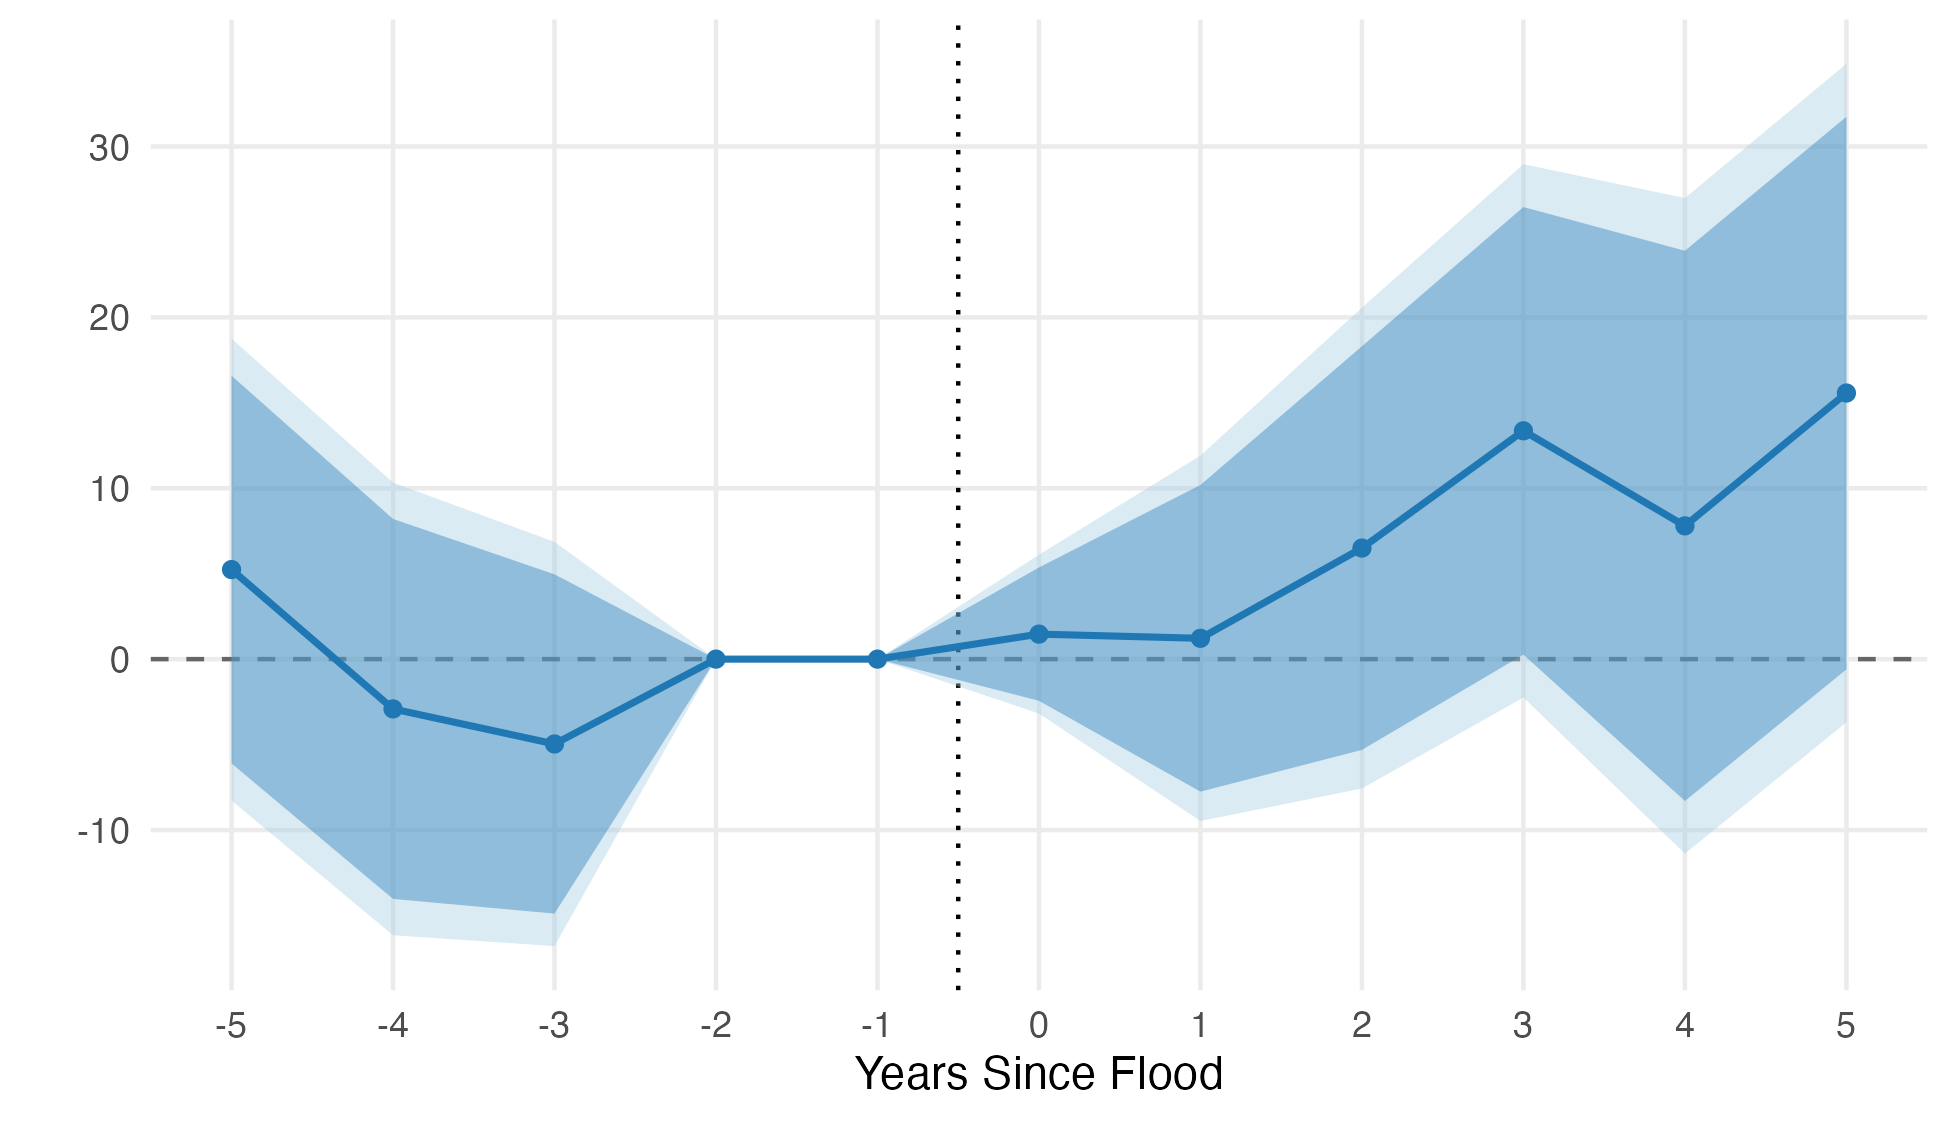
\includegraphics[width=0.45\textwidth]{figures/Results/Analysis_Communes/litorale/IRF_EFF_3112_litorale_0.png}
    \hspace{1em}
    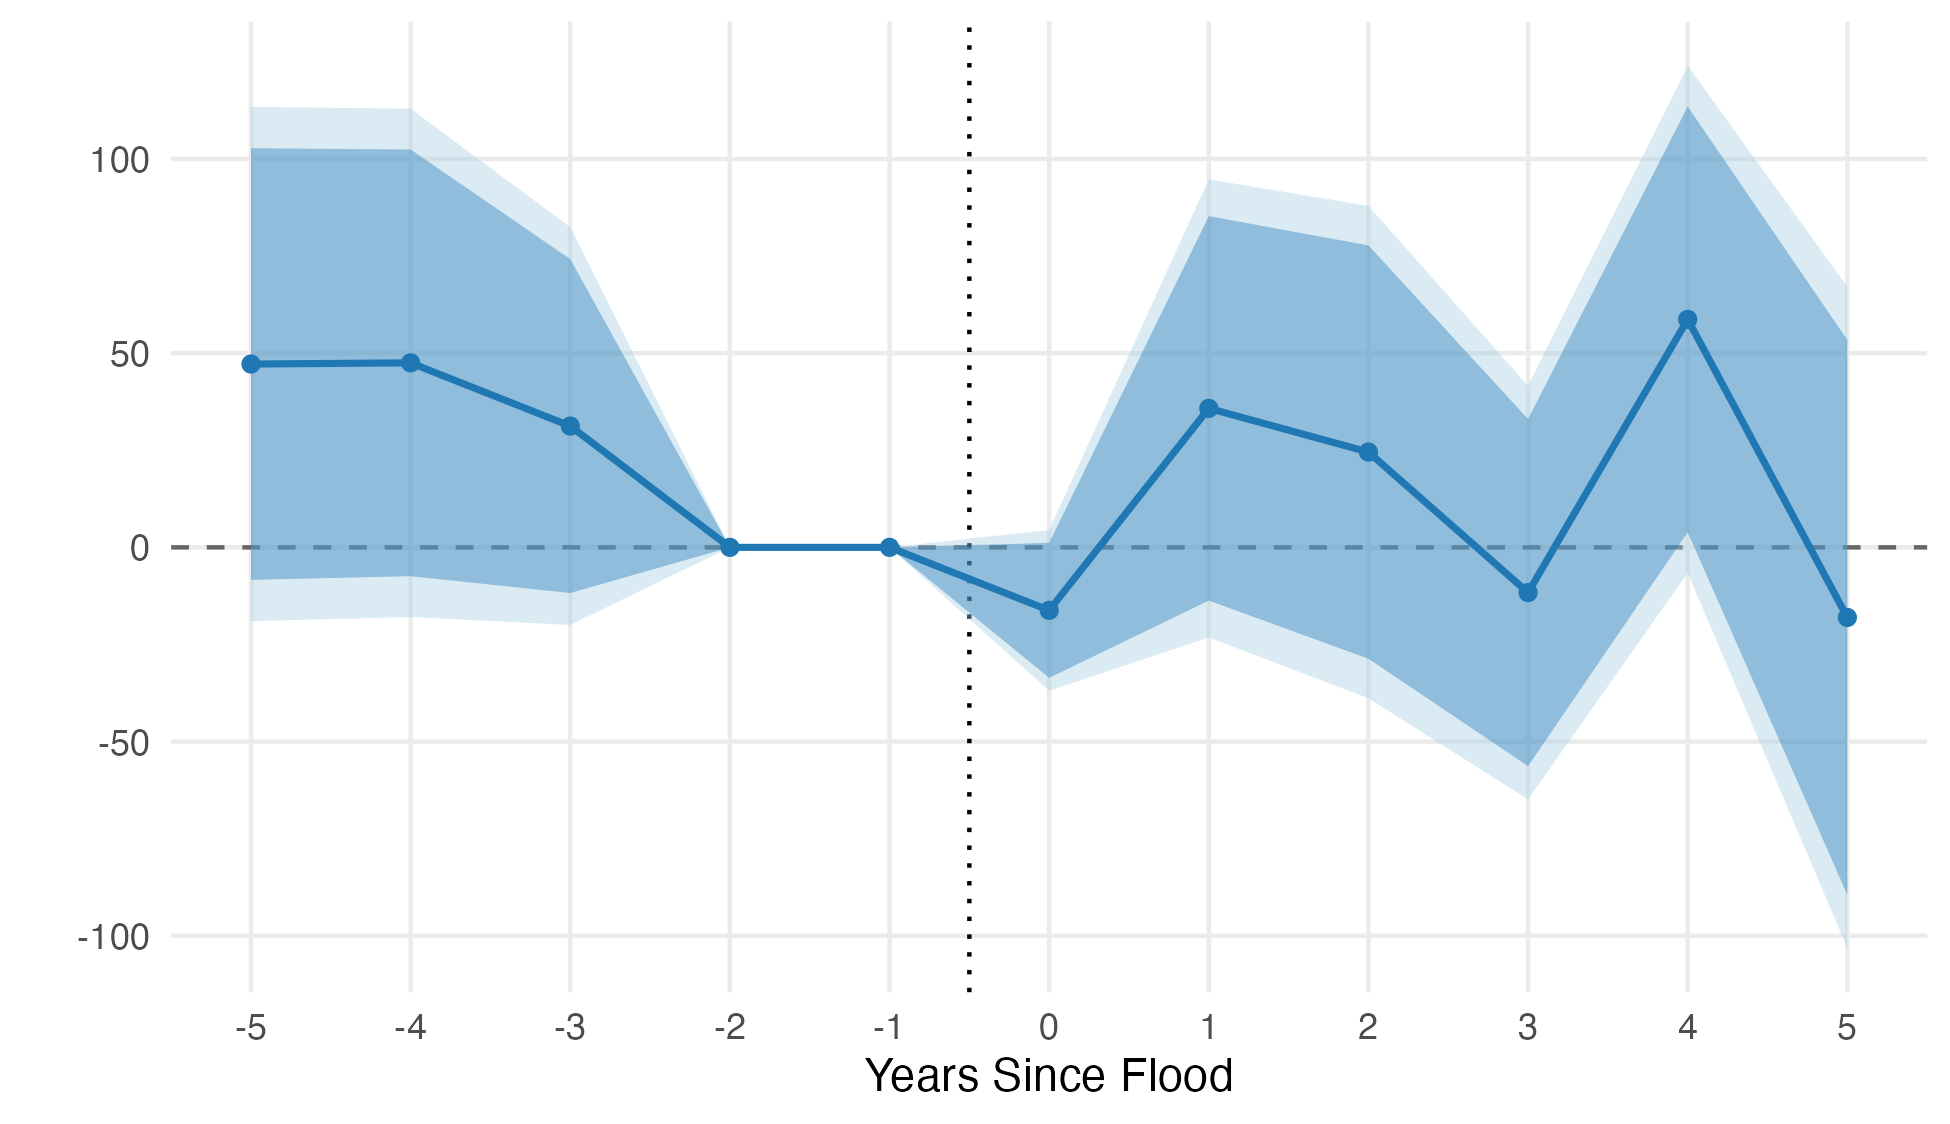
\includegraphics[width=0.45\textwidth]{figures/Results/Analysis_Communes/litorale/IRF_EFF_3112_litorale_1.png}
    \subcaption{Headcount at 31.12}
  \end{subfigure}

  \vspace{1.2em}

  % Row 2: AVGWAGE3112
  \begin{subfigure}[b]{\textwidth}
    \centering
    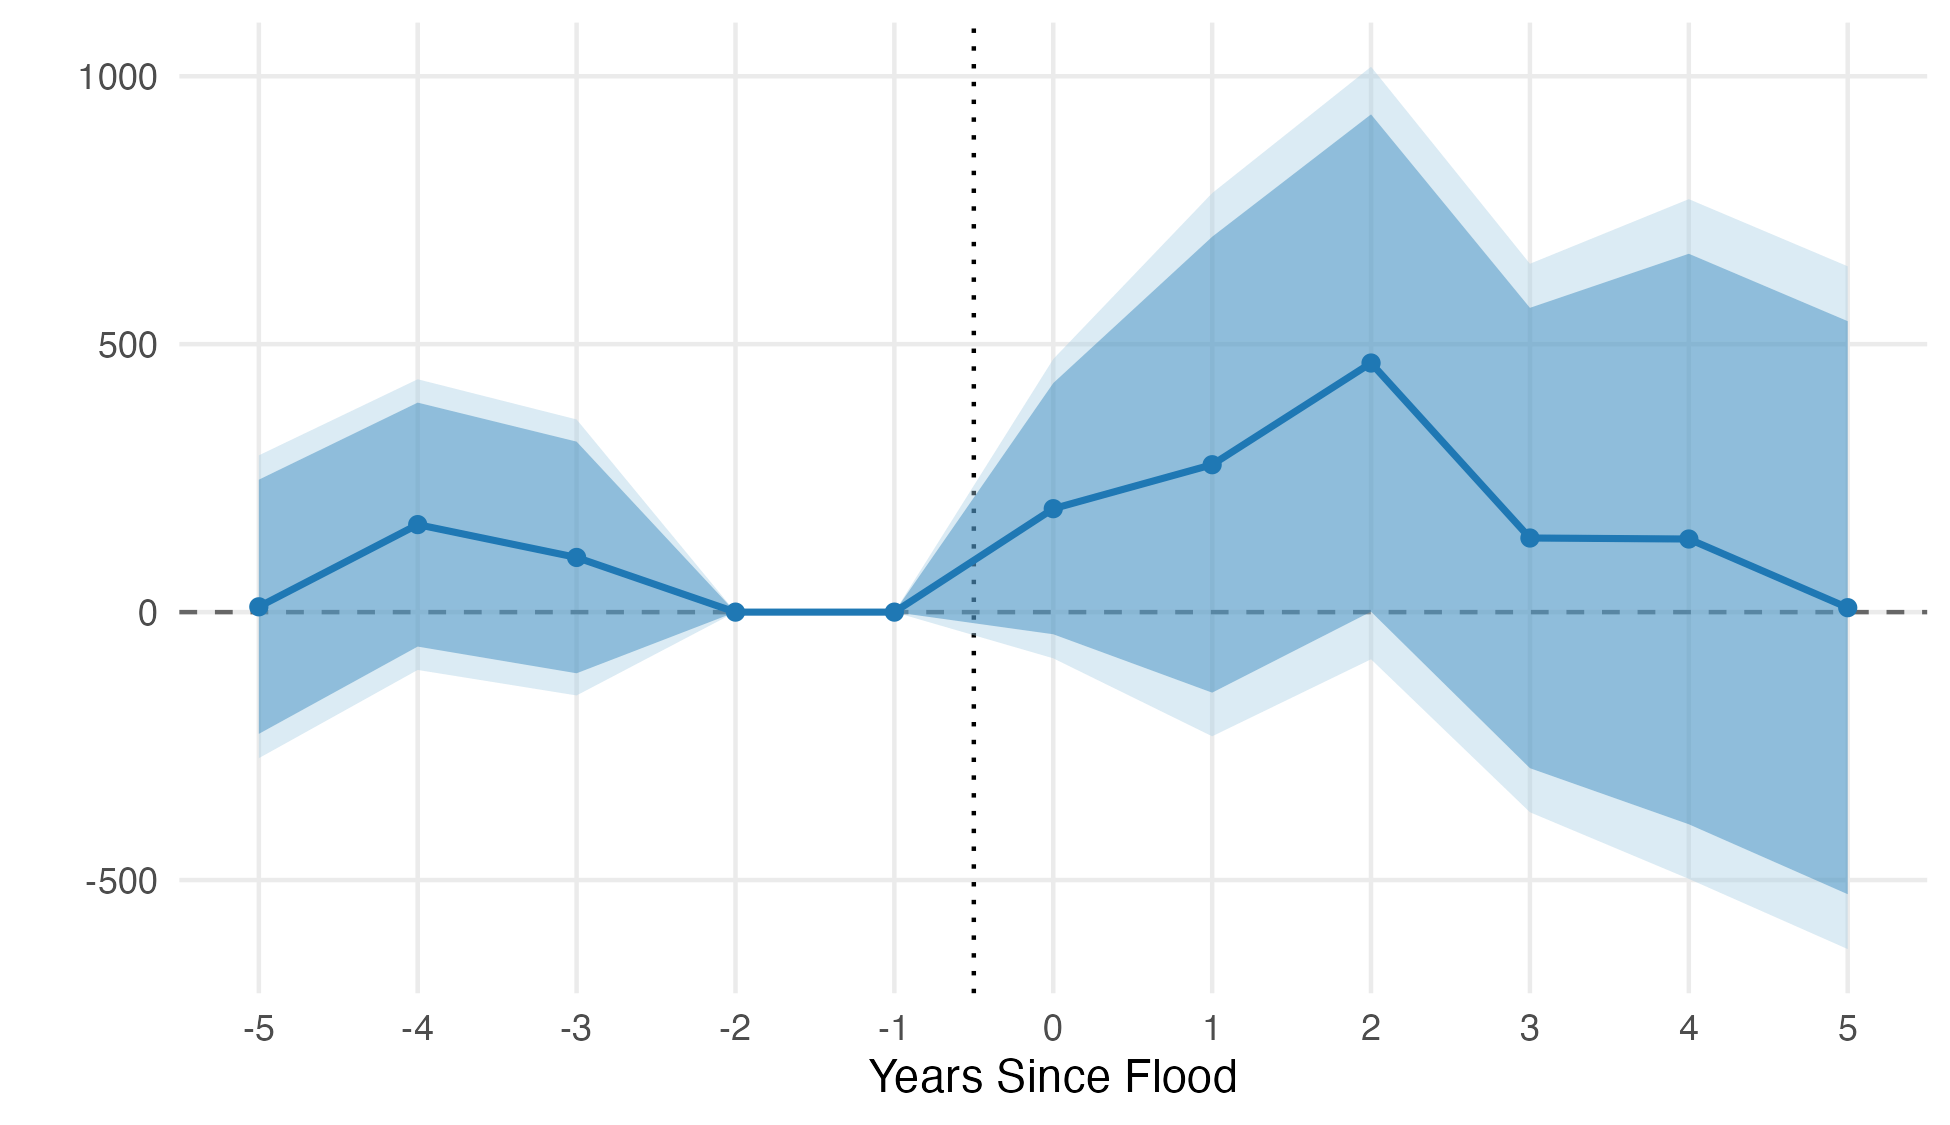
\includegraphics[width=0.45\textwidth]{figures/Results/Analysis_Communes/litorale/IRF_AVGWAGE_litorale_0.png}
    \hspace{1em}
    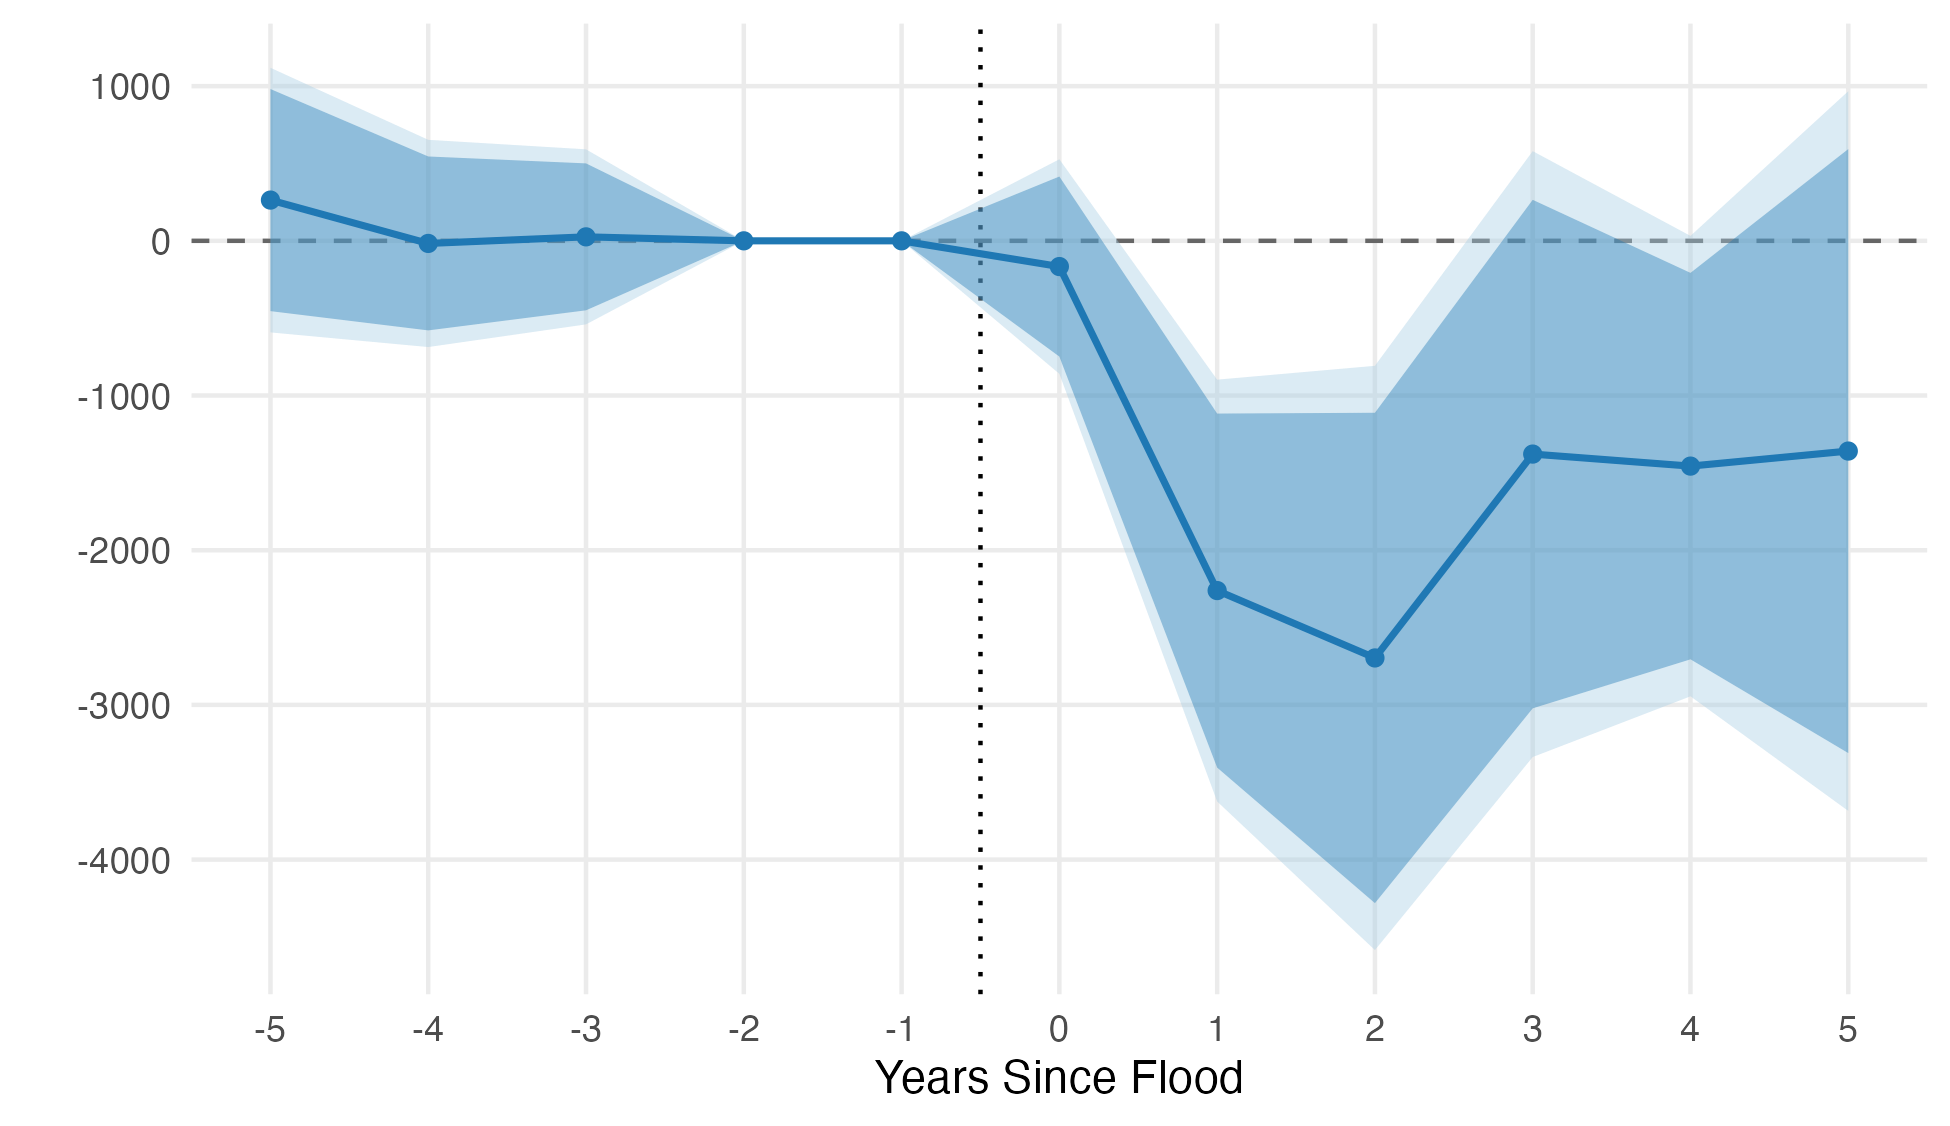
\includegraphics[width=0.45\textwidth]{figures/Results/Analysis_Communes/litorale/IRF_AVGWAGE_litorale_1.png}
    \subcaption{Wages at 31.12}
  \end{subfigure}

  \vspace{1.2em}

  % Row 3: Revenue
  \begin{subfigure}[b]{\textwidth}
    \centering
    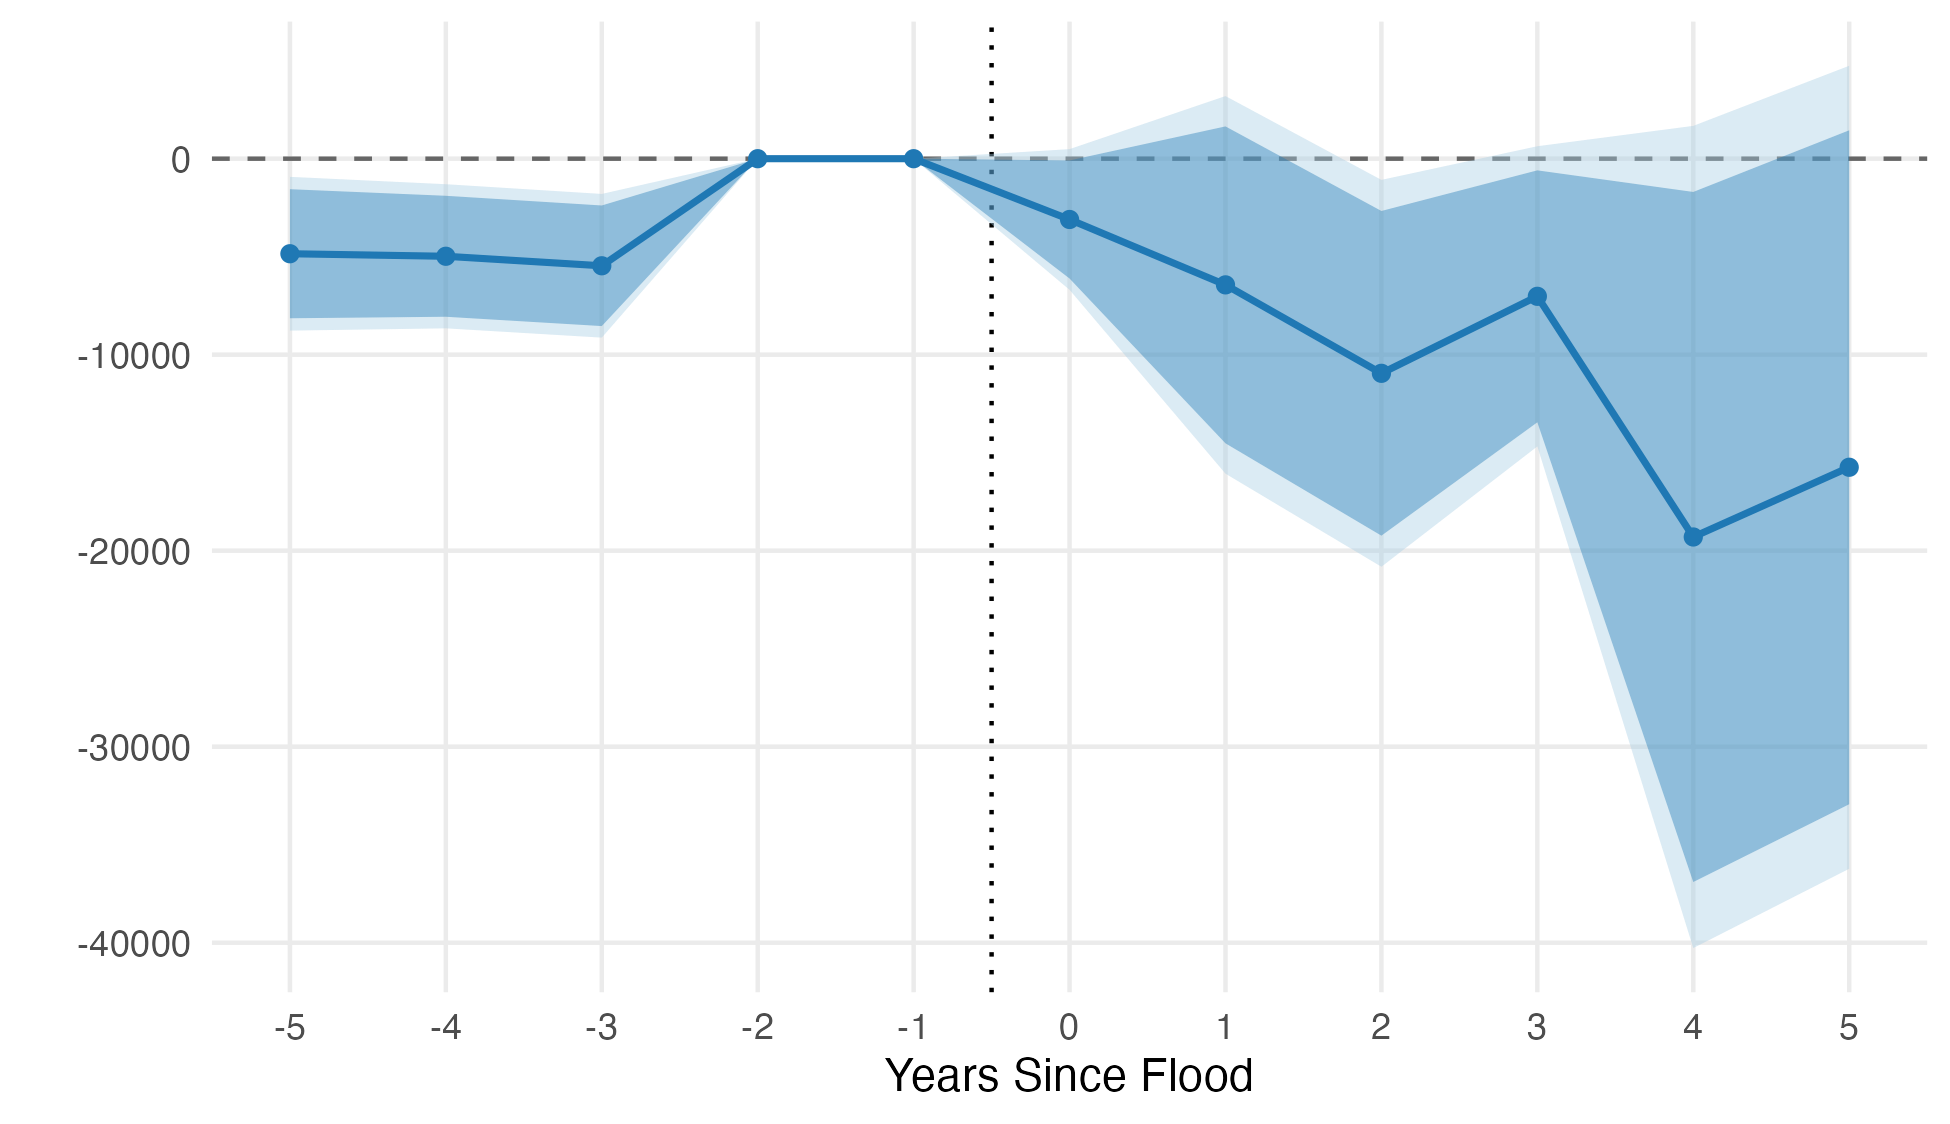
\includegraphics[width=0.45\textwidth]{figures/Results/Analysis_Communes/litorale/IRF_redi_r310_SIRET_litorale_0.png}
    \hspace{1em}
    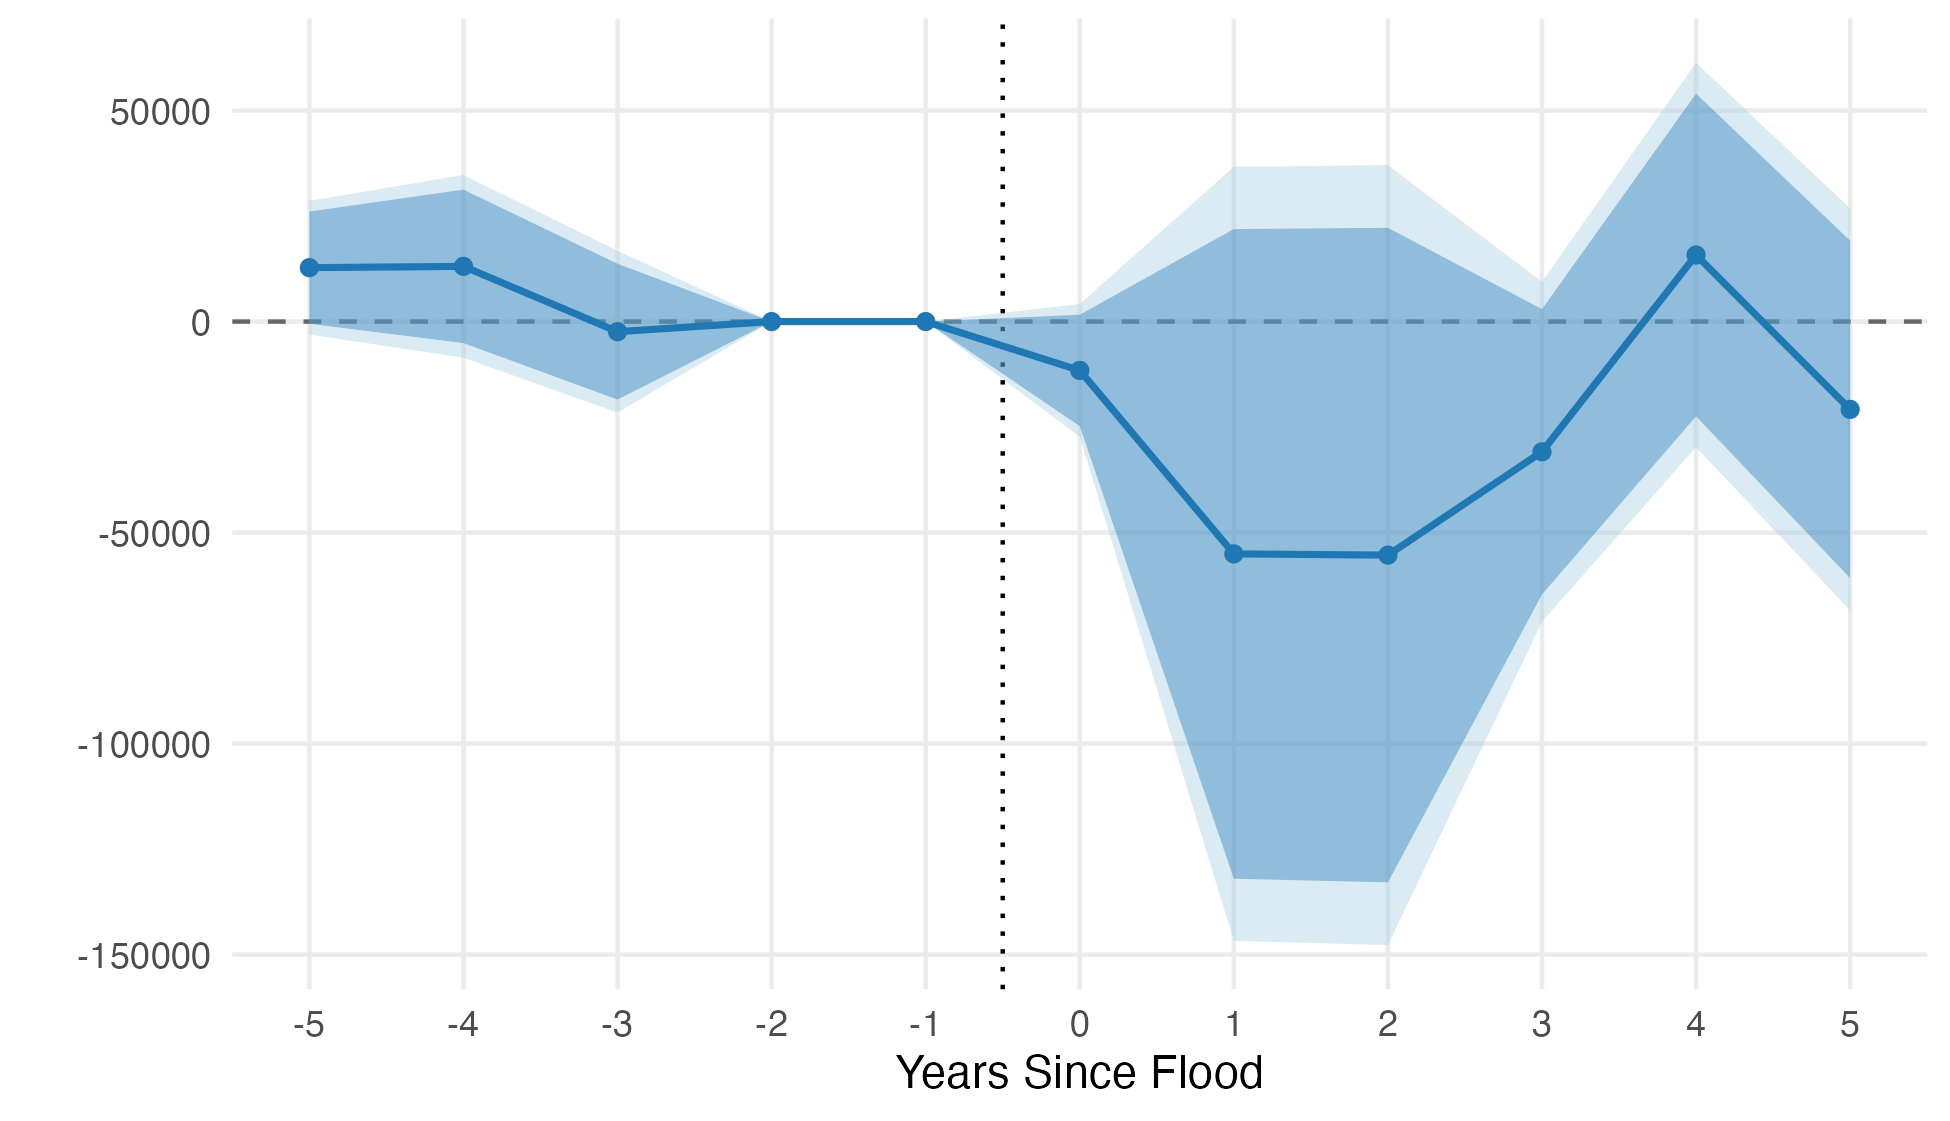
\includegraphics[width=0.45\textwidth]{figures/Results/Analysis_Communes/litorale/IRF_redi_r310_SIRET_litorale_1.png}
    \subcaption{Total Revenue}
  \end{subfigure}
   \caption*{\raggedright\textit{Note}:  Shaded areas indicate 90\% and 95\% confidence intervals. The first flood for a commune is defined as the first year in which the commune witnessed a \textit{CatNat} flooding episode in the sample. Since the outcomes data starts in 2010 but the floods can be tracked since 1985, only those communes that did not witness any flood event in the period 2000-2009 are included in the analysis. To get to the aggregate variables from establishment-level information, the variables are then summed across communes for each year using labor share weights.}
\end{figure}

To examine heterogeneity, I stratify communes by coastal exposure. Figure \ref{fig:IRF_litorale_comparison} shows that coastal communes experience somewhat larger short-term declines in revenues and wages following floods, whereas non-coastal communes exhibit flatter trajectories. The confidence intervals remain wide, so these patterns should be interpreted with caution. Still, the comparison suggests that exposure to the sea amplifies short-run damages, consistent with physical vulnerability and higher baseline flood risk in coastal areas.\\

This designation of a flooding episode is place-based, tied to the specific communes affected, and primarily triggers compulsory insurance coverage for damages sustained. It does not automatically unlock substantial public funding for infrastructure reconstruction or direct fiscal transfers to households and firms. Nevertheless, it ensures regulated insurance payouts, offering financial relief to those affected. \cite{indaco2021hurricanes} find a similar mechanism at work in the U.S. hurricane context, where insured losses are quickly compensated but public transfers play only a minor role.
Other mechanisms may also explain why aggregate effects appear muted. First, CCR insurance payouts cushion establishment-level losses and provide immediate liquidity, preventing wider economic dislocation. Second, firm entry and exit dynamics can rebalance local activity, with new entrants or expanding firms offsetting losses from those directly affected. Third, labor mobility between communes of work and residence helps smooth employment adjustments, as workers can shift jobs or commute elsewhere even if their local establishment is disrupted. Fourth, land use and cementification patterns condition how economic activity is exposed to flooding, with more built-up areas often facing higher direct damages but also faster recovery due to greater infrastructure and capital intensity. Finally, labor market regulation and unemployment insurance shape how shocks are absorbed: where firing costs are high, firms may adjust via capital rather than layoffs, while workers benefit from income smoothing through insurance or temporary withdrawal from the labor force.

These findings fit into a broader empirical pattern. \cite{roth2020local} shows that in U.S. counties, unlike hurricanes and tornadoes, floods tend to have a significant negative effect on US counties only in the year of the disaster, followed by a modest positive effect in the medium term, suggesting that aggregate recovery is rapid. \cite{bilal2023anticipating} emphasize that anticipation of climate risks influences location and investment decisions in the U.S., so observed damages may already reflect selection out of the most vulnerable areas. \cite{fatica2024floods} find that in Europe, financial resilience is shaped by insurance institutions and fiscal frameworks, which buffer aggregate outcomes even when establishment-level shocks are severe. Taken together, the evidence indicates that while establishments experience significant disruptions from floods, commune-level aggregates show limited persistent effects, reflecting the role of insurance, reallocation, and recovery mechanisms in attenuating shocks at higher levels of aggregation.

% \textbf{Mechanisms:}
% \begin{itemize}
%     \item CCR payouts
%     \item Firm entry and exit
%     \item perceived flood risk drives selection
%     \item commune of work vs residence: do people still work there or
%     \item Level of cementtifiaction; economic activity like VA is linked to flooding confounders
%     \item Long term scarring of flooding? Labour regulation and (un)employment insurance determine strenght of adjustment mechanisms of workeers and firms. If strong regulation, firms can't fire then adjust in capital. Workers, can switch job if wages go down. Or, workers can adjust by stopping work and training! 
%     \item Cost discoverty
%     \item: 
%     \end{itemize}




% \textbf{Comparison with other effects in the literature:}
% \begin{itemize}
%     \item in \cite{roth2020local}, unlike for other hazards such as hurricane and tornadoes, floods have a significant negative effect on US counties only in the year of the disaster, followed by a modest positive effect in the medium term.  why can't see in financial variablels maybe
%     \item Bilal (anticipating climate chang ein the US)
%     \item Fatica et al (vulnerabilities and resilience to natural disasters in Europe)

%     \item Similar to what other shocks, how can one model these macro done in Bilal, but otherr exapmles if structural models now.
% \end{itemize}


% Read 7 Discussion in Wing stacked, and compare to Dube. I want to talk about ATT and waht exactly I am targeting as estimand.


% Possible Robustness Checks:

% \begin{itemize}

%     \item Vary slightly Flood Risk Index taking into account variation in depth of water in order to categorize chronically exposed areas vs. areas prone to rare but intense flooding
%     \item Sample of mono-establishments only
%     \item include all floods and not only extreme ones
%     \item The spatial scale at which commuting and supply-chain spill-overs are most salient is important, i would like to estimate at ZEMPT level. 
% \end{itemize}

\newpage
\chapter{Discussion}
\label{ch: discussion}

This paper takes a broad view of floods as localized shocks that can propagate through place-specific labor and product markets. Assuming a local general equilibrium perspective as in \cite{kline2014people}, shocks that reduce the demand for labor at a subset of establishments can lower workers’ outside options and can raise effective monopsony power, implying that even modest employment losses translate into welfare reductions larger than the raw employment margin would suggest. My establishment-level estimates point to a persistent decline in end-of-year headcount of roughly 2\% and a fall in end-of-year wages of about 1\%, while hourly wages remain largely unchanged—consistent with an adjustment working primarily through employment timing and contract renewal rather than per-hour productivity. These findings motivate the core normative question of the paper: when do micro shocks cumulate into aggregate damage, and when do insurance, reallocation, and institutions buffer them away?

The answer in my data is a clear micro–macro wedge. At the establishment level, floods cause significant shock; at the commune level, impulse responses are flat and imprecise across outcomes, with only suggestive short-run effects in coastal communes. The contrast between Figure~\ref{fig:IRF_Communes} and the plant-level results underscores that risk-sharing and spatial reallocation are first-order: local demand is buffered, workers commute or switch employers, and unaffected firms expand on the margin. In the coastal split, Figure~\ref{fig:IRF_litorale_comparison} shows somewhat deeper short-run effects for litorale communes, but with wide confidence intervals. Together these patterns rationalize why commune aggregates can look resilient even when establishments experience sizable disruptions.

% The mechanisms consistent with muted aggregates are straightforward. First, the CatNat/CCR architecture acts as an automatic liquidity bridge: compulsory insurance delivers payouts quickly, relaxing cash-flow constraints and attenuating local demand spillovers \citep{grislain2018natural}. Second, entry/exit and intra-commune reallocation shift activity toward less affected producers; third, labor mobility between communes of work and residence smooths employment as workers adjust commuting patterns or re-match; fourth, land use and cementification shape both exposure and recovery speed—dense areas can suffer higher direct damages yet rebuild faster given infrastructure and capital depth; finally, employment protection and unemployment insurance reallocate incidence in the short run, inducing firms to adjust through hours, temporary contracts, or capital rather than permanent separations. In this light, the flat commune-level IRFs in Figure~\ref{fig:IRF_Communes} are an outcome of institutions doing what they are designed to do.

Policy follows directly from this logic. France’s system layers (i) nearly universal insurance via the CatNat scheme, (ii) municipal fiscal responses, (iii) spatial planning through PPRI zoning, and (iv) information infrastructures (Géorisques, ERRIAL, Vigicrues). The first insures cash flow \citep{grislain2018natural}; the second supports public services and small-scale reconstruction \citep{morvan2022municipalities}; the third moves people and capital out of the worst places \citep{CHELLE20251}; the fourth reduces information frictions that otherwise impede private adaptation. Under fat-tailed risk, Weitzman’s argument for precautionary weighting implies that early warning, zoning, and standards can carry large welfare payoffs even when average damages appear modest; empirically, the monetized benefits of European flood warnings are sizable \citep{pappenberger2015monetary}. At the same time, policy can create hazard, such as coastal hazard. For example, large coastal defenses in Jakarta induced relocation into risk, a textbook moral-hazard response \citep{hsiao2023sea}. Good adaptation policy therefore combines insurance and incentives: insure liquidity to avoid inefficient scarring, but price and regulate exposure to reduce chronic risk.

Heterogeneity matters for both inference and design. Vulnerability depends on demographics, land use, and preparedness \citep{boissier2013mortalite,papagiannaki2022developing}. My measurement strategy therefore models intensity using decree duration and conditions on flood history, recognizing that the same hazard can map into different economic losses depending on prior investments and selection. This is squarely in line with recent classifications that cleanly separate hazard, exposure, and vulnerability \citep{kreibich2022challenge}. It also resonates with forward-looking spatial sorting emphasized by \cite{bilal2023anticipating}: if firms and households anticipate risk, observed damages partly reflect selection out of the worst places. Distributional concerns are central: U.S. floodplain regulation varies sharply by income and region \citep{Cano2024Exposing}, and exposure is uneven across occupations \citep{reynier2024distributional}. Flat commune-level averages do not preclude large losses for the least mobile workers and the least diversified, mono-establishment firms—precisely the groups we find to be more vulnerable.

Methodologically, our estimand is the group–time ATT recovered with a stacked/local-projection DiD design that avoids negative-weight pathologies and uses only ``clean'' controls over symmetric windows around first exposure. This choice aligns with best practice when treatment is staggered and anticipatory behavior is plausible \citep{carleton2024adaptation}. Still, several measurement challenges remain. Commune treatment dummies attenuate effects when only a subset of plants are truly flooded; duration-based intensity bins can be biased by reverse causality (productive units drain faster, mechanically shortening measured duration) and by omitted vulnerability (long-duration floods are likelier in low-lying, poorer, agriculture-heavy places). Rich controls and flood-history vectors mitigate but cannot fully eliminate these concerns. Future work should incorporate depth, outage-days, capital retirement, and claims data to refine intensity; track exits explicitly to address survivorship in financial variables; and test robustness to alternative clean-control definitions suggested by the stacked-DiD literature.

The broader comparative evidence is consistent with our micro–macro wedge: for U.S. counties, floods have contemporaneous negative effects followed by modest medium-run rebounds \citep{roth2020local}; in Europe, insurance institutions and fiscal frameworks cushion aggregates even when establishment shocks are severe \citep{fatica2024floods}. Our coastal split echoes this: higher baseline exposure amplifies short-run losses but does not necessarily produce persistent commune-level scarring, again pointing to the importance of institutions and selection. If the policy objective is welfare rather than merely output, the case for action is strongest where outside options are thinnest and liquidity is scarce—that is, where the micro shocks we document are most likely to translate into persistent individual harm even when aggregates recover.

Two practical agendas follow. First, exploit institutional stagger—EAIP (post‑2007) and the expansion of PPRI coverage—to study how protection changes the mapping from hydrology to economic loss; today, roughly three-quarters of the French population live in a PPRI zone, offering quasi-experimental variation at scale. Second, push the spatial unit to economically meaningful labor markets (commuting-zone $\times$ APE) weighting establishments by labor shares to capture spillovers more cleanly. Complement this with mobility analyses using residential data to quantify post‑flood sorting \citep{lethimillock}. On the policy margin, early warnings, storm-water systems, permeable surfaces, and green infrastructure remain high–benefit tools; in agriculture, recent French evidence quantifies sizable adaptation and exposure costs \citep{du2024costs}. For developing countries, where fiscal capacity and governance constraints bind, the economics of adaptation highlights the role for external finance and careful program design \citep{kala2023climate}, while evaluation must explicitly account for anticipatory adaptation \citep{carleton2024adaptation}.

In sum, the paper’s core message is simple. Floods deliver economically meaningful, persistent shocks to establishments; commune-level aggregates, however, look resilient because France’s insurance, fiscal, and regulatory layers reallocate and insure the shock away. The policy task is therefore not only to raise average resilience but to reduce the dispersion of harm: target liquidity and reconstruction support to the most exposed, regulate and price chronic risk, and invest in information and planning that shift people and capital out of harm’s way. Done well—and calibrated to fat tails—this adaptation package yields welfare gains even when aggregate IRFs are flat, precisely because it restores outside options in the places where they are scarcest.


% A large literature studies how geographic shocks reshape local labour markets. \textbf{Situate floods as a negative local productivity shock. Mechanism, Policy, Heterogeneiy.} Following the local-general-equilibrium logic of Kline \& Moretti (2019), the 2\% employment decline we observe translates into substantial welfare loss per worker, suggesting scope for targeted place-based aid..../.how local shocks like floods may deepen monopsony by reducing outside options

% This study helps Develop a theoretical framework that could lead public intervention in this specific field and discuss measures that have been taken to reduce economic losses. difference between risk and uncertainty that in a new global scenario will substantially characterize the reliability of empirical analyses in this complex research field.\\


% In countries severily exposed to coastal flooding, government policies could create climate-hazards such as incentives to relocate in flood-prone areas, this is documented in the case of Indonesia where goovernemnt expenditure to buidl a sea wall induced in coastal moral hazard \cite{hsiao2023sea}. A review of the economics of adapatation in devleoping countries is in \cite{kala2023climate} while the econometrics to estimate the benefits of adaptation are reviewed in \cite{carleton2024adaptation}.  


% Developing countries vs Europe: As the discussion above highlighted, huge investments are related to climate adaptation and mitigation, and for poor countries with less capacity to pay or enforce such mechanisms the role of foreign assistance is important (green finance in the rise), viscious circle of climate and debt. 	
% Also in Europe there is the EU’s Adpatation Policy. Need for industrial policy. Otherwise tragedy of the commons. Does climate change generate windfall profits?	
% Finally, also report on public support for some adaptation measures, e.g., mandatory insurance against floods. This is done for example in Germany in Garbarino et al. (2024), where they elicit households’ preferences for climate adaptation policies. 


% \textbf{Adaptation to floods:} Related to introduction, is that firms' labor demand and firms' financial performance are tightly connected. On one side, employment protection policies could have impact on workers and cushion them. What would be impact on firms performance. On other side, what could be adaptation policies related to firms?
% Then, there are adaptation policies at the commune level in France: municipal spending \cite{morvan2022municipalities}, regulation of land \cite{CHELLE20251}, insurance schemes \cite{grislain2018natural} are all important dimension of public or private adaptation to climate shocks.


% Examples of adaptation are like Bulletin of \href{https://vigilance.meteofrance.fr/fr}{Bullettin meteo france}, live map that the PhD student Julia showed me, \href{https://www.vigicrues.gouv.fr/}{Vigicrues France}. Since 2003, France requires sellers and landlords to inform buyers and tenants about known local risks, a measure reinforced in 2022 by mandating disclosure directly within property listings; \href{https://www.georisques.gouv.fr/consulter-les-dossiers-thematiques/dossier-expert-sur-les-inondations}{ERRIAL}, a dedicated online platform, supports this transparency by providing free parcel-level risk reports, thereby facilitating climate adaptation by reducing information asymmetry between property owners and buyers. Citizens in France have various ways to have access to accurate flood risk information: public risk maps (Géorisques Portal (georisques.gouv.fr)); government data (local authorities (préfecture and mairie)), and private modeling (International risk-modeling firms, Real estate consultancies); real-estate disclosures (IAL – Information des acquéreurs et des locataires; “ERP” – État des Risques et Pollutions).




% These protections—common in certain European countries—function as implicit insurance for workers and local demand, while potentially imposing costs on firms. This reframes employment protection as a climate adaptation instrument, not just a labor market institution.


% \textbf{Political economy of climate adaptation} 
% Just as legislative frameworks like PPRI affect land use, tax credits and deductions affect incentive of adaptive techonology, and other, labor market institutions shape post-disaster firm-worker dynamics. Employment-protection measures such as require firms to retain workers during periods of work stoppage, e.g., due to physical inaccessibility or power outages), or restrict dismissals in the aftermath of disasters are common in certain European countries and function as implicit insurance for workers and local demand, while potentially imposing costs on firms.


% The paper also echoes your mention of Weitzman and others on precautionary regulation in uncertain environments.

% Discuss also \href{https://scholar.harvard.edu/files/stock/files/cost_of_delaying_action.pdf}{Weitzman’s Dismal Theorem}, then (Yasmine Van Der Straten  Enrico Perotti  Frederick Van Der Ploeg), then in the french context: Douvinet's Les maires face aux plans de prevention du risque inondation (PPRI). The point is that as explained in introduction and Boissier, the context is important and legilsative frameworks (non structural) measures are \emph{crucial influencing factors on the spatial and temporal evolution of flood risk and its management, and thus important determinants of outcomes and the impacts of floods.}FINAL (e.g., legislative frameworks comparisons across countries is found in (Serra‐Llobet et al. 2022, Managing) 
% s

% The monetary benefit of early flood warnings in Europes

% Examples of flood adaptation; improved storm water management systems, better urban planning, more accessible early warning systems and growing investments in green infrastructure, like replacing concrete surfaces with more permeable materials or planting more trees; as our infrastructure was built for a climate that no longer exists,”

% \textbf{Costs and benefits of adaptation}: For example, \cite{pappenberger2015monetary} estimate a very high cost benefit ratio of investing in flood prevention in Europe. In the french context, \cite{du2024costs} examine in the case of agriculture. The impact of floods on french municipal budgets is exminaed in \cite{morvan2022municipalities}. 

% page 9 carleton, criique to my reduced form esiamtes as not so informative o pollicymakers!

% \textbf{Related to section where i describe why I create flood-intentisy dummy and flood exposure in bins (22 days), and generally to need to constrol for flood history:} vulnerability to flooding can depend on many things, as pointed out in \cite{boissier2013mortalite} in the French context and \cite{papagiannaki2022developing} in the European context, so that a same measure of exposure (e.g., wather depth, estimated damages) can imply different effects, based on precautionary behavior or firm characteristics. The A recent Nature article (Kreibich et al (2022)) classifies exposure. This highlights how climate adaptation is not yet well understood. 



% To conclude, the breadth and variety of insurance possibilities fundamentally shape prevention decisions and recovery dynamics in the aftermath of flooding. Across the world, the public health response, access to credit, the existence of insurance mechanisms, and the extent of ex-ante adaptation undertaken all play a role. The spatial distribution of flood exposure bears in itself distributional issues. This is documented in the U.S., where floodplain regulations have been shown to vary sharply by income level and region \citep{Cano2024Exposing}, while exposure is also uneven across occupations \cite{reynier2024distributional}.

% \cite{lethimillock} docuents residents going out. Clarifying such interaction between measurable charactetiecsics, governance mechanisms that work and long-term flood vulnerabilty measures (see Kornik) is essential for judging whether existing financing tools remain fit for purpose in an era of warming temperatures and fat-tailed risk. 


% \textbf{Further Research}:

% EAIP was created in 2007, it would be interesting also to study the staggered adoption of these ``protection" zones on areas that are geophysically simialr. Also, PPRI, and today \href{https://www.georisques.gouv.fr/minformer-sur-la-prevention-des-risques/les-risques-naturels-en-france-chiffres-cles#:~:text=Plus%20de%2012%20500%20communes,pr%C3%A9vention%20Inondation%20(hors%20submersion%20marine)}{74,4\%} of french popiulation lives in a zone covered b a PPRI. THen TRI.. Residential mobility responses to home damage caused by floods


% Main Limitatitons:

% \begin{itemize}
%     \item Binary dummies waste information; specification should allow for depth bins of flooded area or a measure by damages. This could be done exploiting the duration days in another way. CCR does not publish damages for each flood.
%     \item measiring damages incurred as proxy of flood intenty, and days of power outage; for services, days of worker absence,.. cool
%     \item Possible bias in terms of like angrist: Reverse causality / simultaneity	Firms or farmers with robust infrastructure pump water out quickly. Their outcome (high output) shortens measured duration.	Productive units look like they faced a “milder” flood, so you understate true flood harm.
%     \iteem Omitted variables (“bad controls”)	Places that sit in the ≥ 23-day bin are often low-lying, poor, or agriculturally intensive. Those same factors also depress income, health, or productivity even without a flood.	The long-duration dummy soaks up both flood damage and persistent disadvantage → upward-biased damage estimates.
%     \item considering all firms impacted within a commune: downward bias
% \end{itemize}


% Discuss econometrics; Check page Table A2 in stacked paper, where illustrates how these different clean control definitions matter when analyzing. One can do based on the standard sample inclusion
% criteria we have used throughout her paper; strict clean
% controls inclusion criteria (s > a+ > post + >pre), where we omit any not yet treated group who has pre-period data that falls within our pre bound; only never treated units are used as clean controls.
\newpage
\chapter{Conclusion}
\label{ch: conclusion}


Flooding is set to remain a lasting challenge in France. A recent report by Réseau Action Climat (RAC) and Ademe \cite{RAC2024} provides a detailed region-by-region assessment of France’s changing climate landscape, highlighting diverse climatic risks and vulnerabilities. Compared to the IPCC’s global outlook, these assessments are more local in scale, and thus directly relevant for adaptation: they fill knowledge gaps where policy must operate. France’s \emph{Plan national d’adaptation au changement climatique} (PNACC), whose Measure 3 explicitly targets flooding, is one such framework, but its implementation has often been uneven and interrupted—underscoring the difficulty of sustaining long-term climate governance.

At the European level, recent debates—such as those raised in the Draghi Report—stress that climate policy cannot be separated from industrial policy. A green industrial strategy is increasingly necessary to overcome adaptation and mitigation barriers. In this regard, Earth observation systems such as Copernicus provide comprehensive, real-time data for environmental and climate monitoring, while new investments in green infrastructure and innovation are central to Europe’s adaptation capacity.

It is important to recognize that the very notion of a “natural disaster” is not neutral. As the vulnerability paradigm emphasized since the 1970s, disasters are not solely the result of extreme environmental events but also of socio-economic and political conditions that make certain groups more susceptible to harm \citep{nations2010natural}. The IPCC’s Sixth Assessment Report similarly stresses that changes in the frequency or magnitude of hazards do not directly translate into changes in risk if proactive management—such as protection or managed retreat—is undertaken \citep{Reisinger2020Concept}. In this sense, what appears as a sudden disaster is in fact the culmination of long-term exposure, behavior, and institutional choices. Climate change exacerbates these dynamics by introducing non-stationarity into natural systems, making past data a less reliable guide for future adaptation.

The urgency of this issue is underscored by recent events. The European State of the Climate 2024 reports that nearly one-third of Europe’s river network flooded last year \citep{copernicus2024esotc}. In France, October 2024 floods in the Auvergne–Rhône–Alpes region brought 600 mm of rain in just 48 hours—roughly Paris’s annual total—triggering widespread evacuations, crippling infrastructure, and leading the Ministry for Ecological Transition to relaunch the PNACC. Meteo France described the episode as the most intense rainfall over two days since the early 20th century. Similar catastrophic floods in Spain, Germany, and the Netherlands further illustrate the rising risks posed by climate extremes across Europe.

In light of the empirical evidence presented in this paper—showing that floods generate substantial microeconomic disruptions but muted aggregate effects—the conclusion is clear: institutional design matters. Insurance, fiscal buffers, spatial planning, and public information can prevent localized shocks from cascading into systemic crises. Yet climate change is intensifying the scale and frequency of hazards, and adaptation policies must be calibrated to fat-tailed risks, not historical averages. The challenge for France and Europe is to ensure that climate adaptation is not reactive but anticipatory, linking climate policy, industrial policy, and social protection. Doing so will not only reduce aggregate losses but also, crucially, limit the unequal distribution of harm across communities, workers, and firms.



% Flooding in France is here to remain, \href{https://reseauactionclimat.org/la-france-face-au-changement-climatique-toutes-les-regions-impactees/}{report by Réseau Action Climat (RAC)} and Ademe provides a detailed region-by-region assessment of France's changing climate landscape, highlighting diverse climatic risks and vulnerabilities. More local than IPCCC, so this is also a magin of adaptation: filling knowledge gaps. Also, the Plan national d'adaptation au changement climatique (PNACC) Measure 3 directly concerns flooding and it says.. 




% Draghi rport:, and industrial strategy for Europe to overcome these barriers; applying a climate policy without an industrial policy, indutriall policis on the rise  

% In Earth Observation, Copernicus offers the most comprehensive
% data worldwide, including for environmental and climate change monitoring, disaster management and security.


% Economics of catastrophes: Global Priorities Institute \\

% Science Po Syllabus \\


% We should not take for granted that it is a disasdter, but ask: What made it so? In Switzerlannd, Blatten was not a disaster because all were evvacuated!\\

% Ethimology of ``disaster" pag. 54 of pdf Disaster Studies \\

% A green innovation/industrial policy for Europe (Reinhilde Veugelers) \\




% \textbf{The notion of natural disaster:} Because both reactive and proactive actions can influence the ultimate impact of natural disasters, the notion itself of “natural disaster” is an analytical conceit that needs interpretation. As a rupture of the socio-economical order, a natural disaster is triggered by environmental forces but is ultimately an historical process rooted in the path-dependent ways economic and governance institutions change. This recognition led to the emergence in the 1970s of the \textit{vulnerability} paradigm in reaction to the then dominant \textit{hazard} paradigm, shifting the focus from the hazard event itself to the underlying conditions that make certain groups more susceptible to harm, highlighting how natural disasters are the cumulative implications of many earlier decisions, some taken individually, others collectively \citep{nations2010natural}. Hence the idea of “natural Hazards, unnatural disasters. In the IPCC's Sixth Assessment Report the notion of Risk \citep{Reisinger2020Concept} is pointed out that changes in the frequency and/or magnitude of climatte hazards do not map directly changes in actual risk if socio-economic changes like proactive risk management decisions such as protection or managed retreat are met. These is an important point to keep in mind when considering the distributional impacts of clilmate adaptation policies, as well as the estimation of damages from disasters. To conclude, what appears as a sudden “disaster” is in fact the result of an historical process deeply embedded in pre-existing patterns of exposure and behavior. As a consequence, structural exposure to natural disasters is not random, rather is rooted in long-term social and spatial processes. Climate change further exacerbates these issues as it introduces non-stationary in the distributions of many natural systems and makes climate patterns no longer stable or predictable based on past trends, a point we will return to later. \\



% \textbf{Recent floods in Europe}
% The \emph{European State of the Climate 2024} reports that almost one-third of the continent’s river network flooded last year \citep{copernicus2024esotc}, and recent deadly floods across Europe are a reminder of the growing threat of climate-induced extreme weather events. 
% Recent floods in France in October 2024 in the Auvergne-Rhône-Alpes region, delivering up to 600 mm of rain in 48 hours in the Ardèche departmeent only roughly Paris’s annual total triggering 900 evacuations and crippling rail and power infrastructure emmploying 3 000 sapeurs-pompiers and the ministry for Ecological transition called for the Relaunch of the National Climate Change Adaptation Plan (PNACC) previously stopped. The most intense ever recorded over two days since the beginning of the 20th, said Meteo France! \href{https://www.franceinfo.fr/replay-radio/le-grand-temoin/intemperies-des-moyens-massifs-toujours-deployes-selon-le-ministre-delegue-a-la-securite-du-quotidien_6816923.html}{France Info}. In neighouringh european countriesr such as Spain, Germany, and the Netherlands recent destructive floods are a reminder of the growing threat of climate change-induced extreme weather events. 

% Banchmark across countries and shared learning is very important: netherlands has an adanced flood anagmetnn sstemms due to histotry, and U we can learn: they do sponge parks and rain tunnel, sopraeleveate houses (in france evelstion of flood walls, works performed on th ebed of rivers, and the creation of reservoir lakes..).




\newpage

%%%%%%%%%%%%%%%%%%%%%%%%%%%%%%%%%%%%%%%%%%%
% Bibliography
%%%%%%%%%%%%%%%%%%%%%%%%%%%%%%%%%%%%%%%%%%%
\pagenumbering{Roman} %Roman numbering for the last pages
\setcounter{page}{5}

\bibliographystyle{apacite}
\bibliographystyleinternet{apacite}
 
 %References are directly linked to my web library from Zotero
 
\bibliography{references.bib}
 
% \bibliographyinternet{references.bib}

%%%%%%%%%%%%%%%%%%%%%%%%%%%%%%%%%%%%%%%%%%%
% Appendices
%%%%%%%%%%%%%%%%%%%%%%%%%%%%%%%%%%%%%%%%%%%
\appendix

\renewcommand{\thefigure}{A\arabic{figure}}  % Prefix all figure numbers in appendix with "A"
\setcounter{figure}{0} 

\renewcommand{\thetable}{A\arabic{table}}  % Prefix appendix tables with "A"
\setcounter{table}{0} 

\chapter*{\LARGE Appendices}


\addcontentsline{toc}{chapter}{Appendices}
% Temporarily adjust tocdepth so sections do not appear in the main TOC
\addtocontents{toc}{\protect\setcounter{tocdepth}{-1}}
\renewcommand{\thesection}{\Alph{section}}
\adjustmtc 
% mini table of contents for appendices
\minitoc
% Restore normal tocdepth for sections within the appendices
\setcounter{tocdepth}{2}

%%%%%%%%%%%%%%%%%%%%%%%%%%%%%%%%%%%%%%%%%%%%%%%%%%
%%%%%%%%%%%%%%%%%%%%%%%%%%%%%%%%%%%%%%%%%%%%%%%%%%
\section{Data descriptions and variable creation details}
%%%%%%%%%%%%%%%%%%%%%%%%%%%%%%%%%%%%%%%%%%%%%%%%%%
%%%%%%%%%%%%%%%%%%%%%%%%%%%%%%%%%%%%%%%%%%%%%%%%%%


This section details how the data used in this paper was collected and processed. I describe in turn the data sources mentioned in Table \ref{tab:data_sources}. The codebook (Table \ref{tab:codebook}) serves as further reference.

%%%%%%%%%%%%%%%%%%%%%%%%%%%%%%%%%%
\subsection{GASPAR Database}

In the raw GASPAR database, each row corresponds to a single hazard clause of a natural catastrophe decree published in the \textit{Journal Officiel}—that is, one commune, one hazard, and one time window. Each decree is identified by a unique code CatNat, but when multiple hazards are recognized within the same decree (e.g. both flooding and landslides), the identifier is repeated, generating one row per hazard. As a result, raw counts of code CatNat overstate the number of distinct events. To avoid this double-counting, I collapse the data to the commune × hazard × calendar-year level, treating all rows that share these three keys as a single disaster episode within a commune. The resulting event counts are reported in Table \ref{tab:flood_summary}. Figure \ref{fig:durat_categories} plots the distribution of durations for all recorded flood events, which serves as the basis for defining my three categories of flood intensity. \\
%It would be interesting to plot here trend in GASPAR CatNat and Floods CatNats, disuss how this could be biased. i alrady did that graph.


  \begin{figure}[htbp]
    \centering
    \caption{\textbf{Figure \ref{fig:durat_categories}:}  Distribution of flood event durations}
    \label{fig:durat_categories}
    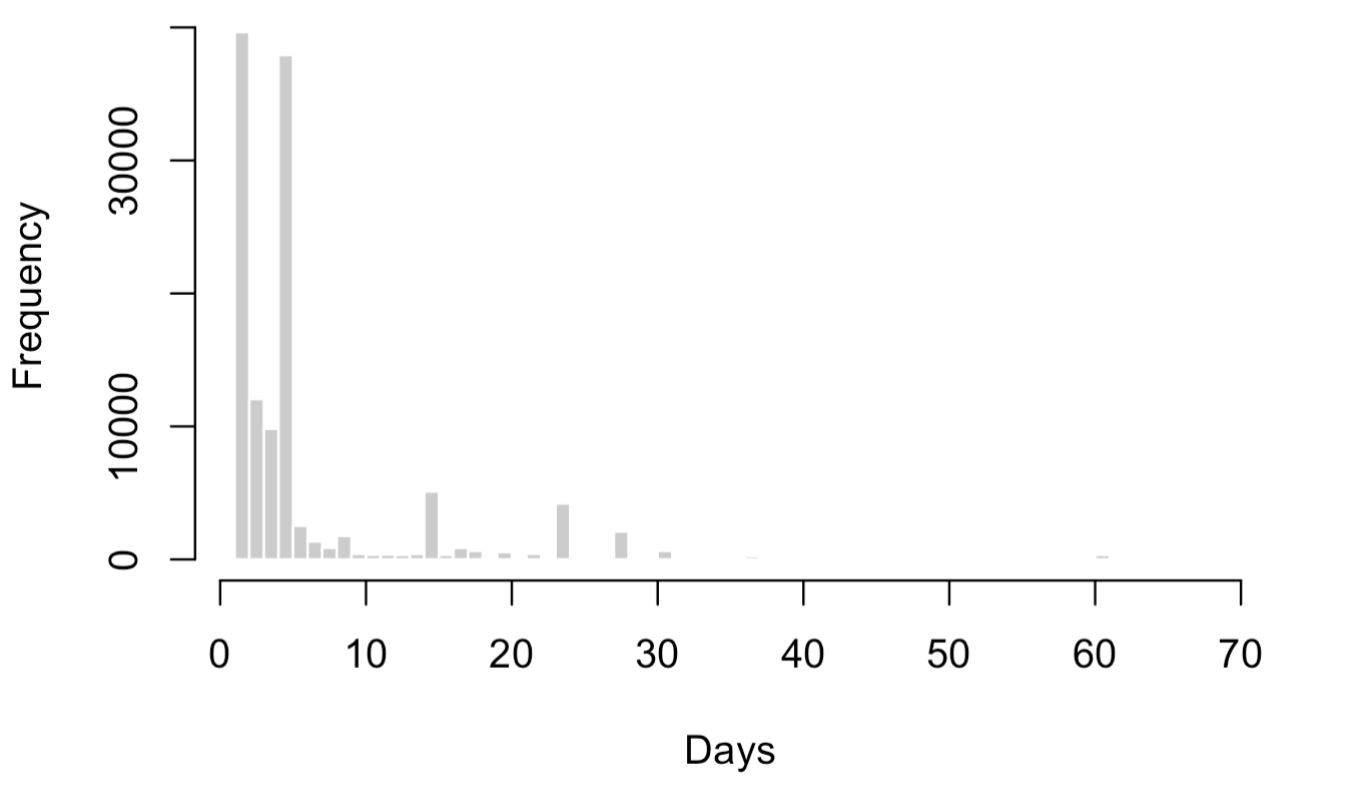
\includegraphics[width=0.9\textwidth]{figures/Data/duration_flood_gaspar.png}

    %\caption*{\raggedright\textit{Note}:}
    
    \end{figure}


%%%%%%%%%%%%%%%%%%%%%%%%%%%%%%%%%%%
\subsection{Long Term Flood Exposure Index}
\label{ch:appendix_risk_index}


\noindent
Utilizing high‐resolution floodplain maps of Europe provided by \citet{dottori_et_al_2022}, I propose and develop a time-invariant flood risk index that is used to stratify the econometric analysis and guide sample selections. I choose the floodplain map with RP100 floods, indicating the extent of flooding that is statistically expected to be equaled or exceeded on average once every 100 years, a standard return period used in insurance and urban planning. I overlay the RP100 raster (GeoTIFF) data—a grid of 90m × 90m cells, each with a continuous value of water depth (in meters)—onto the polygons of all communes in metropolitan France. Counting how many of the raster cells fall within the boundaries of a commune, and then converting cell counts to surface areas, allows me to compute the percentage share of a commune's total area that is exposed to varying intensities of flood risk. Following categorization schemes used by the European Commission’s \href{https://drmkc.jrc.ec.europa.eu/risk-data-hub#/}{Risk
 Data Hub} and in the PESETA reports, I classify exposure intensity of each raster cell into four bands: $(0–0.5m]$, $(0.5–1.5m]$, $(1.5–3m]$, and $>3m$. The distribution of water depth values is heavily right-skewed, as shown in Figure \ref{fig:raster_values_distrib}. For each commune, the risk index is simply built as the sum of four variables, capturing the proportion of the commune’s total surface falling into each of the four depth bands, and excluding “unflooded” remainder. The risk index thus ranges from 0 to 100, and is plotted in Figure \ref{fig:risk_index}; it can be conceived as the share of each commune’s surface that is colored in purple in Figure \ref{fig:raster_unbinned}. Several flood risk or exposure indices are used in the academic literature—alongside \cite{indaco2024adapting} and \cite{hussain2024flooding}. Other indices range from global event-based \citep{okazawa2011development}, local exposure-vulnerability \cite{anindita2020flood}, GIS susceptibility models, to composite social-exposure indices and macro-scale global indices (WorldRiskIndex). These indices go in the direction of the damage function in \cite{carleton2022valuing} and, more specifically for our application, the damage functions in \cite{bilal2023anticipating}.

This measure of flood hazard could be refined in several ways. Rather than relying on a simple sum of flooded area across intensity categories, a weighted sum—placing greater emphasis on more severe flooding—would better reflect the nonlinear relationship between water depth and economic damage often observed in engineering and insurance data \cite{ballocci2024econometric}. For example, a commune that is 30\% flooded at 2 meters likely faces far greater losses than one that is 100\% flooded at 5 cm. Similarly, exploiting multiple return periods (e.g., RP10 vs. RP500) would allow the index to capture temporal variation in exposure, distinguishing between persistently exposed areas and those facing latent, tail risks. These “risk-jumpers” can be identified by subtracting RP10 from RP500 flood depths—a difference that preliminary analysis has shown to be minimal in most regions but notable in places like the Loire Valley around the city of Orléans, highlighting the importance of such hazard maps in informing investments in resilience across France. As explained in Section \ref{ch: discussion}, to improve precision of my estimates, beyond the risk index I include other time-invariant covariates in my specification, such as the share of establishments covered by EAIP (Figure \ref{fig:eaip_map}) and commune median revenue. I also test other covariates that could have been included directly in the index. Table \ref{tab:pscore_logit} shows results.

%Table X reports the share of communes classified as “risk-jumpers” (large RP500 vs. RP10 exposure) by region versus those under chronic risk, as well as other statistics around the risk index (including correlation with CatNat events). 

Finally, in integrated structural models of climate change, a flood risk index at the commune level could act as an amenity shifter that affects the relative desirability of locations. Households and firms are assumed to sort spatially based on wages, prices, and local amenities, influencing spatial sorting and long-run equilibrium under evolving climate risk. By simulating these equilibria under different flood scenarios (e.g., comparing RP10 vs. RP500), the model can generate forward-looking predictions of where people and firms are likely to concentrate or retreat. %offering a powerful tool for long-term planning and adaptation policy.
\vspace{0.3cm}

\begin{figure}[!htbp]

  \centering
  % first subfigure at 49% of text width
  \caption{\textbf{Figure \ref{fig:raster_flood}:} Hazard exposure - Flood raster data (RP100)}
  \label{fig:raster_flood}
  \begin{subfigure}[b]{0.44\textwidth}
    \centering
    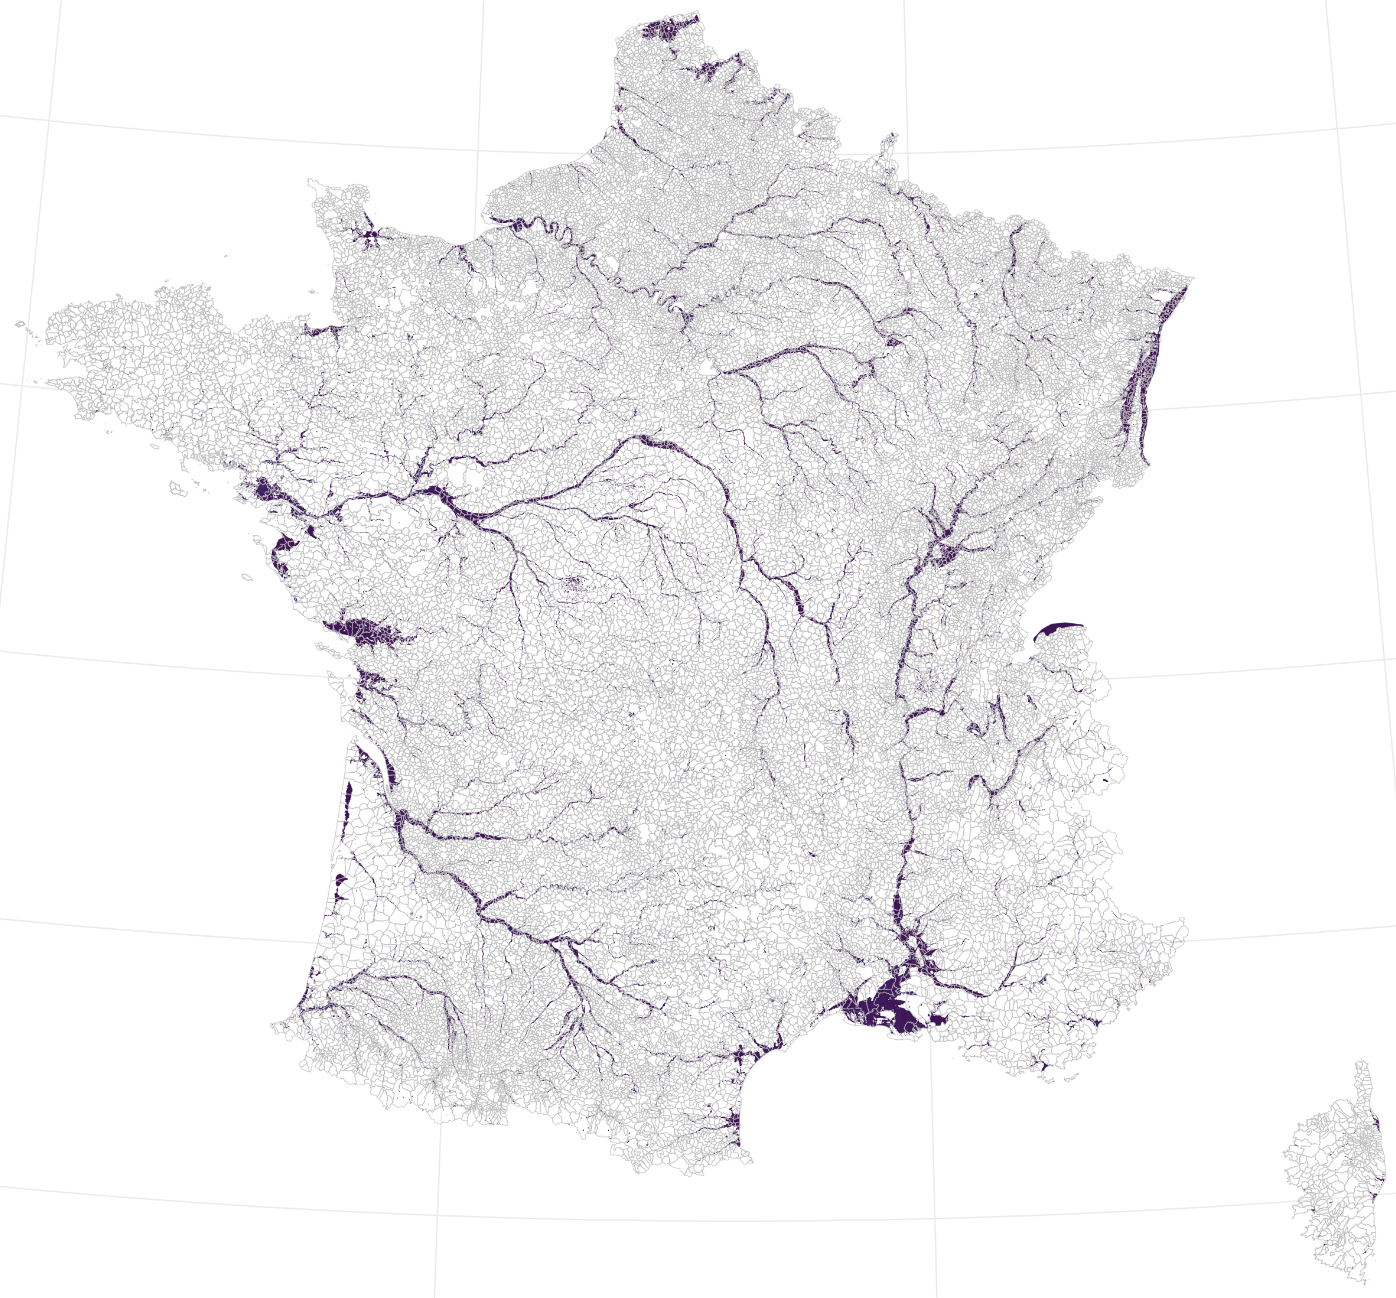
\includegraphics[width=\linewidth]{figures/Data/Raster Unbinned.png}
    \subcaption{Extensive margin of ex-ante risk}
    \label{fig:raster_unbinned}
  \end{subfigure}%i
  % tiny horizontal skip, then second
  \hspace{0.02\textwidth}%
  \begin{subfigure}[b]{0.536\textwidth}
    \centering
    
\includegraphics[width=\linewidth]{figures/Data/Raster Binned.png}
    \subcaption{Intensive margin of ex-ante risk}
    \label{fig:raster_binned}
\end{subfigure}



\end{figure}


\begin{figure}[!htbp]
    \centering
    \caption{\textbf{Figure \ref{fig:raster_values_distrib}:} Histogram of RP100 flood‐depth values at 90m×90m resolution}
    \label{fig:raster_values_distrib}
    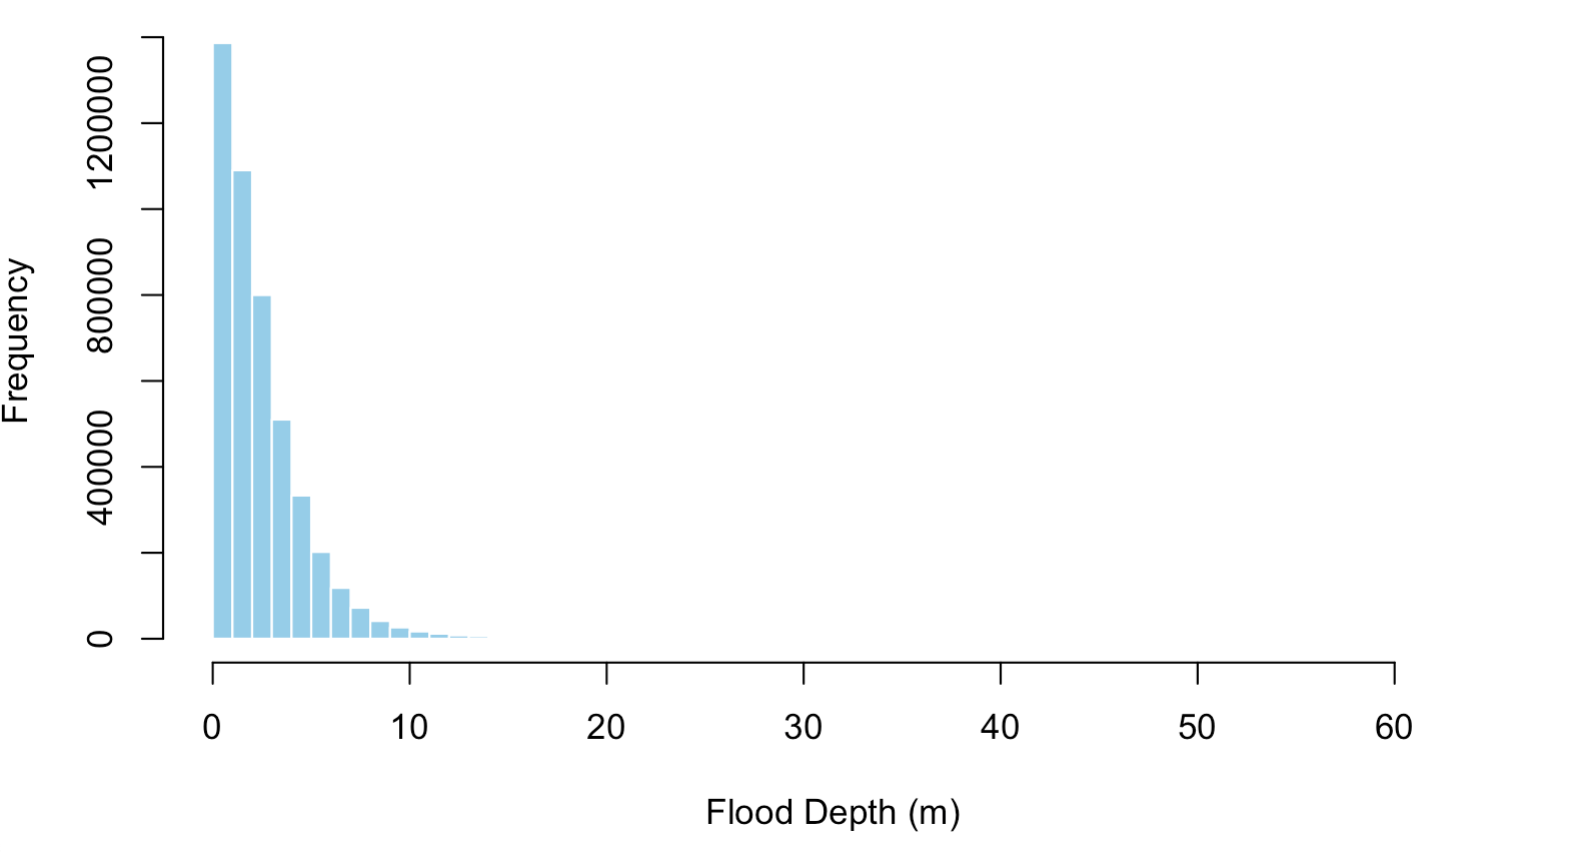
\includegraphics[width=0.7\textwidth]{figures/Data/Raster depth values.png}
    \caption*{\raggedright\textit{Note}: The distribution is markedly right-skewed: the vast majority of pixels record minimal inundation, while a small tail captures the comparatively rare, deeper flood depths. Furthermore, 90\% of all flooded cells fall between 0.07 and 3 meters in water depth.}
    
    \end{figure}


\begin{figure}[!htbp]
    \centering
    \caption{\textbf{Figure \ref{fig:risk_disribu}:} Histogram of Flood Risk Index values at commune level}
    \label{fig:risk_disribu}
    
    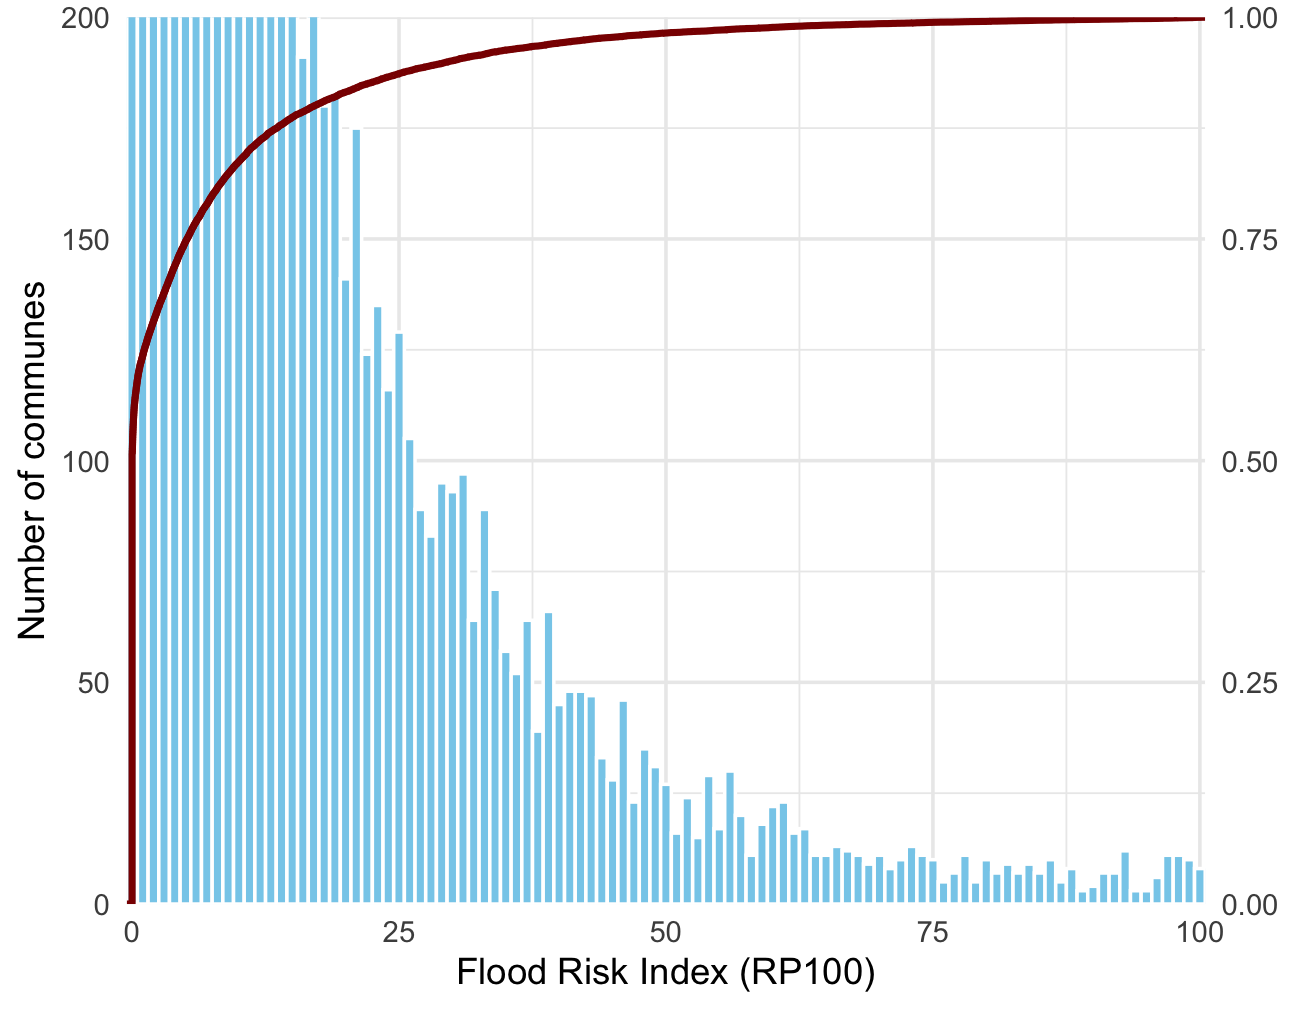
\includegraphics[width=0.7\textwidth]{figures/Data/disribution risk index.png}
    %\caption*{\raggedright\textit{Note: The distribution of the index}}
    
    \end{figure}













%%%%%%%%%%%%%%%%%%%%%%%%%%%%%%%%%

\subsection{Propensity Score}
\label{ch:pscore_appendix}
To improve covariate balance between treated and control firms, and hence precision, I estimate a propensity score for flood exposure using pre-determined firm and location characteristics, following a specification similar to \cite{fatica2024floods}.

As long as unconfoundedness is assumed and common support is established, IPW estimators can be used to estimate ATE and ATT effects. While ATE weights ask what would happen if a randomly selected firm were flooded, ATT weights estimate how floods affected firms that were actually flooded. Given my interest in realized flood shocks, I focus on the ATT. I examine the distribution of the propensity score across treatment status. I then use the score to construct analytical weights. The ATT weights are of the form:

\noindent\text{weights given by}
\begin{align*} w_1^{att}(D) &= \frac{D}{\mathbb{E}[D]}, \\ w_0^{att}(D, p(X)) &= \frac{\frac{(1 - D)p(X)}{1 - p(X)}}{\mathbb{E}\left[ \frac{(1 - D)p(X)}{1 - p(X)} \right]}. \end{align*}

I begin with a pooled logit that relies only on time-invariant firm characteristics, whose result is presented in Table \ref{tab:pscore_logit}. Once the propensity score is known, I build the ATT weights as described above and proceed with standard inference procedures, re-estimate the outcome model on this re-weighted sample. The distribution of $p(x)$ in the adjusted and unadjusted sample is shown in Figure \ref{fig:pscore_distr}, while Figure \ref{fig:ps_cov_balance} illustrates the improvement in covariate balance achieved by the computed weights.

\vspace{1cm}

\begin{table}[!htbp] 
\centering 
\caption{\textbf{Table \ref{tab:pscore_logit}:} \textsc{Propensity-score logit for extreme floods (2010–2019)}} 
\label{tab:pscore_logit}

 \resizebox{12cm}{!}{
\begin{tabular}{@{\extracolsep{6pt}}p{8cm} c} 
\\[-1.8ex]\hline 
\hline \\[-1.8ex] 
& \textit{Dependent variable:}\\ 
\cline{2-2} 
\\[-1.8ex] & Extreme-flood dummy\\ 
\hline \\[-1.8ex] 
Flood–risk-group decile            & 0.160$^{***}$ \\ 
                                   & (0.029)        \\[0.15em]

Share of establishments under EAIP & 0.219          \\ 
                                   & (0.280)        \\[0.15em]

Income category of commune         & 0.0334         \\ 
                                   & (0.088)        \\[0.15em]

Urban dummy                        & 0.456$^{***}$  \\ 
                                   & (0.073)        \\[0.15em]

Coastal dummy (littoral sea)       & 0.908$^{***}$  \\ 
                                   & (0.127)        \\[0.15em]

Floods 1982–1999 (count)           & $-$0.118$^{***}$ \\ 
                                   & (0.044)        \\[0.15em]

Constant                           & $-$3.476$^{***}$ \\ 
                                   & (0.206)        \\[0.35em]
\hline \\[-1.8ex] 
Observations                       & 6,676,631       \\ 
Wald $\chi^2$(6)                   & 178.33          \\ 
Pseudo R$^2$                       & 0.0293          \\ 
Log pseudolikelihood               & $-$1,564,659.3  \\ 
\hline 
\hline \\[-1.8ex] 
\multicolumn{2}{p{13cm}}{\textit{Note:} $^{*}p<$0.1; $^{**}p<$0.05; $^{***}p<$0.01. Robust standard errors clustered at the commune level. Coastal dummy includes only sea-type areas (89\% of cases). Interestingly, the coefficient for floods occurring in 1982–1999 is negative, possibly indicating that adaptation to flooding has taken place in communes more heavily exposed in the past, now resulting in fewer CatNat declarations.} \\ 
\end{tabular}}
\end{table}

% , the next steps are: 1) convert the obtained propensity scores to IPW (ATE) or ATT weights, then compute MSD in the IPW-weighted data so that treated and control groups share the same covariate distribution, and ; 2) apply doubly-robust IPW-RA; 3) nearest-neighbor matching, pairing each flooded commune with the dry commune that has the closest propensity score and computing the mean outcome gap within those matched pairs; 4) drop units whose predicted score is near 0 or 1, keeping only the range where both treated and control communes exist, then run the analysis on that trimmed sample.

% Since I cannot estimate ATE (there is selection into treatment), I estimate ATT effects. The weights are built as $\frac{e_i}{1-e_i}$ for controls. Balance is shown after matching.



% \noindent To capture common calendar-year shocks and unobserved heterogeneity across firms, one could also estimate a more nuanced model such as:

% \begin{equation}
% \Pr!\bigl(D_{it}=1 ,\big|, X_i, T_t, u_i\bigr)=
% \Phi!\Bigl(\alpha X_i+\delta T_t+u_i\Bigr)
% \end{equation}

% This would allow estimation of a more accurate propensity score.


\begin{figure}[htbp]
\centering
\caption{\textbf{Figure \ref{fig:ps_cov_balance}:} Covariate balance before and after matching}
\label{fig:ps_cov_balance}
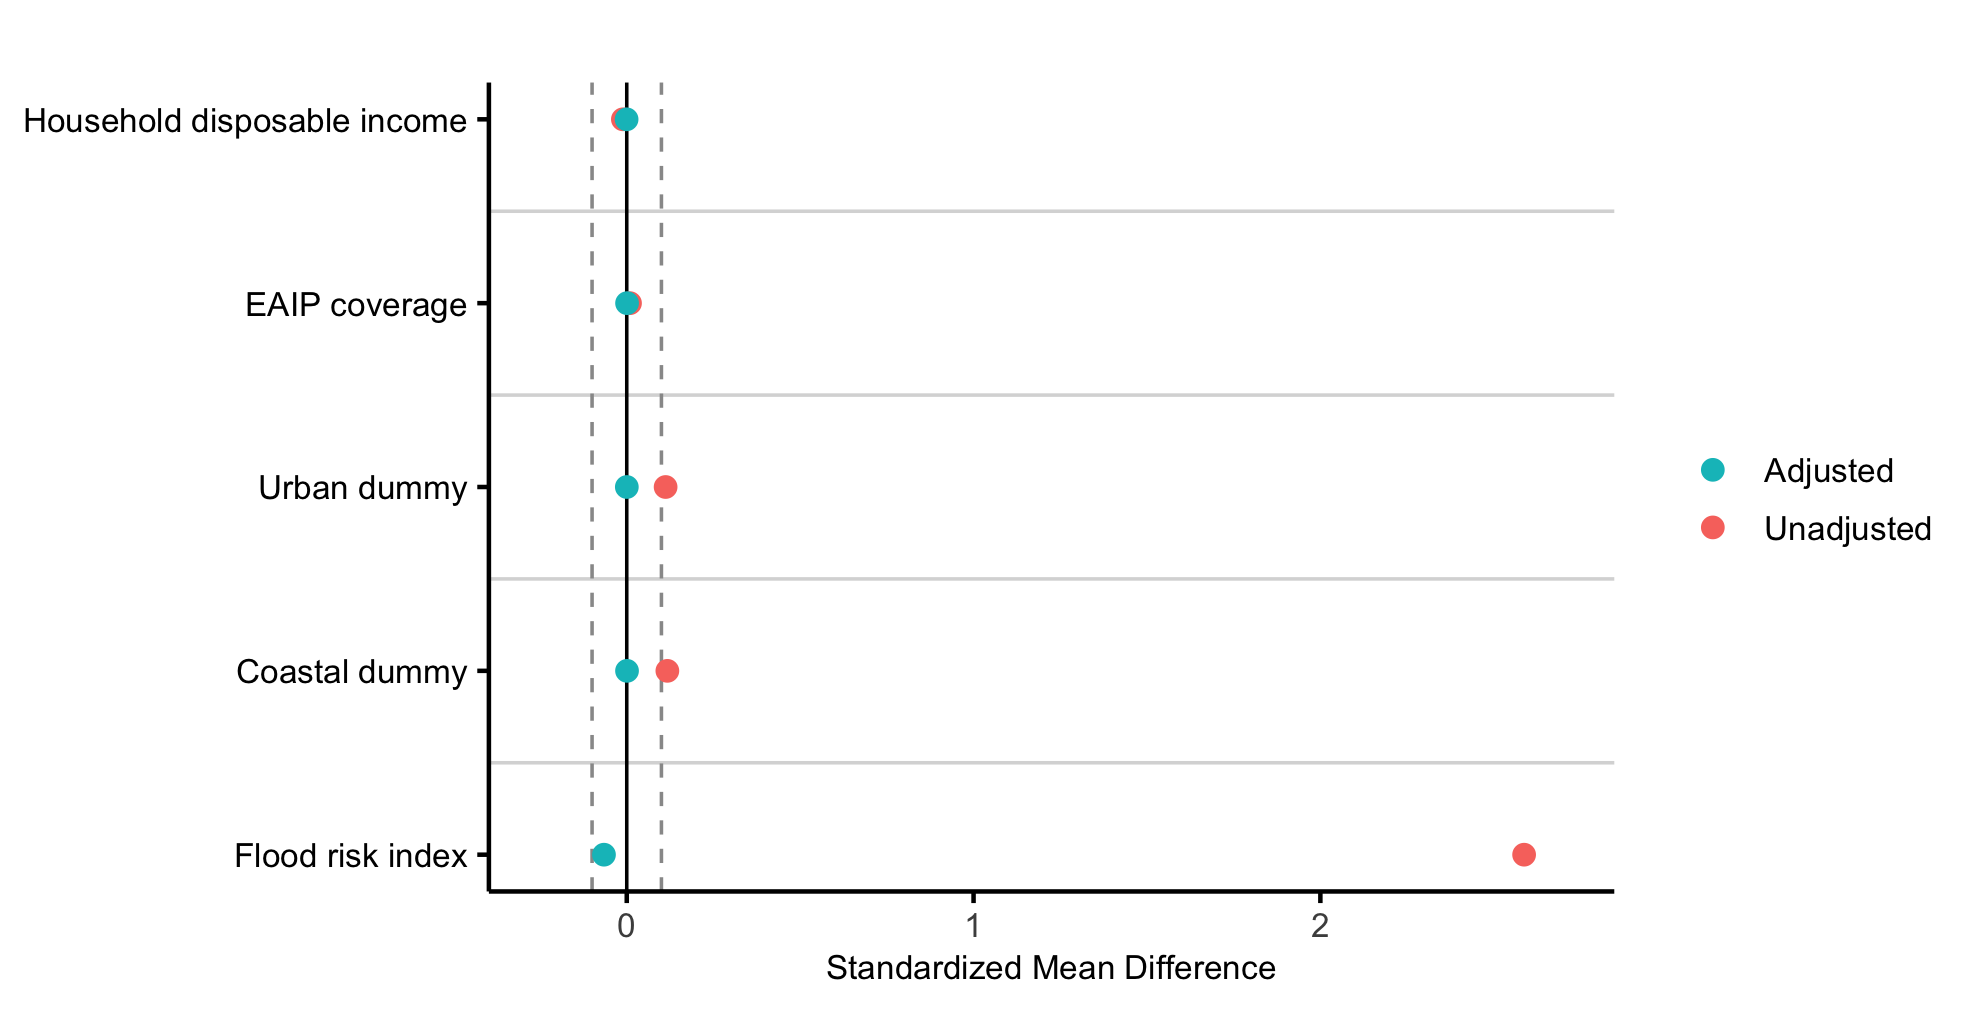
\includegraphics[width=0.86\textwidth]{figures/PScore/covariate_balance.png}
\caption*{\raggedright\textit{Note}: Flood risk index is an outlier with 2.59 SMD in the unadjusted sample.}
\end{figure}

\vspace{0.2cm}

\begin{figure}[htbp]
\centering
\caption{\textbf{Figure \ref{fig:pscore_distr}}: Propensity score distribution}
\label{fig:pscore_distr}
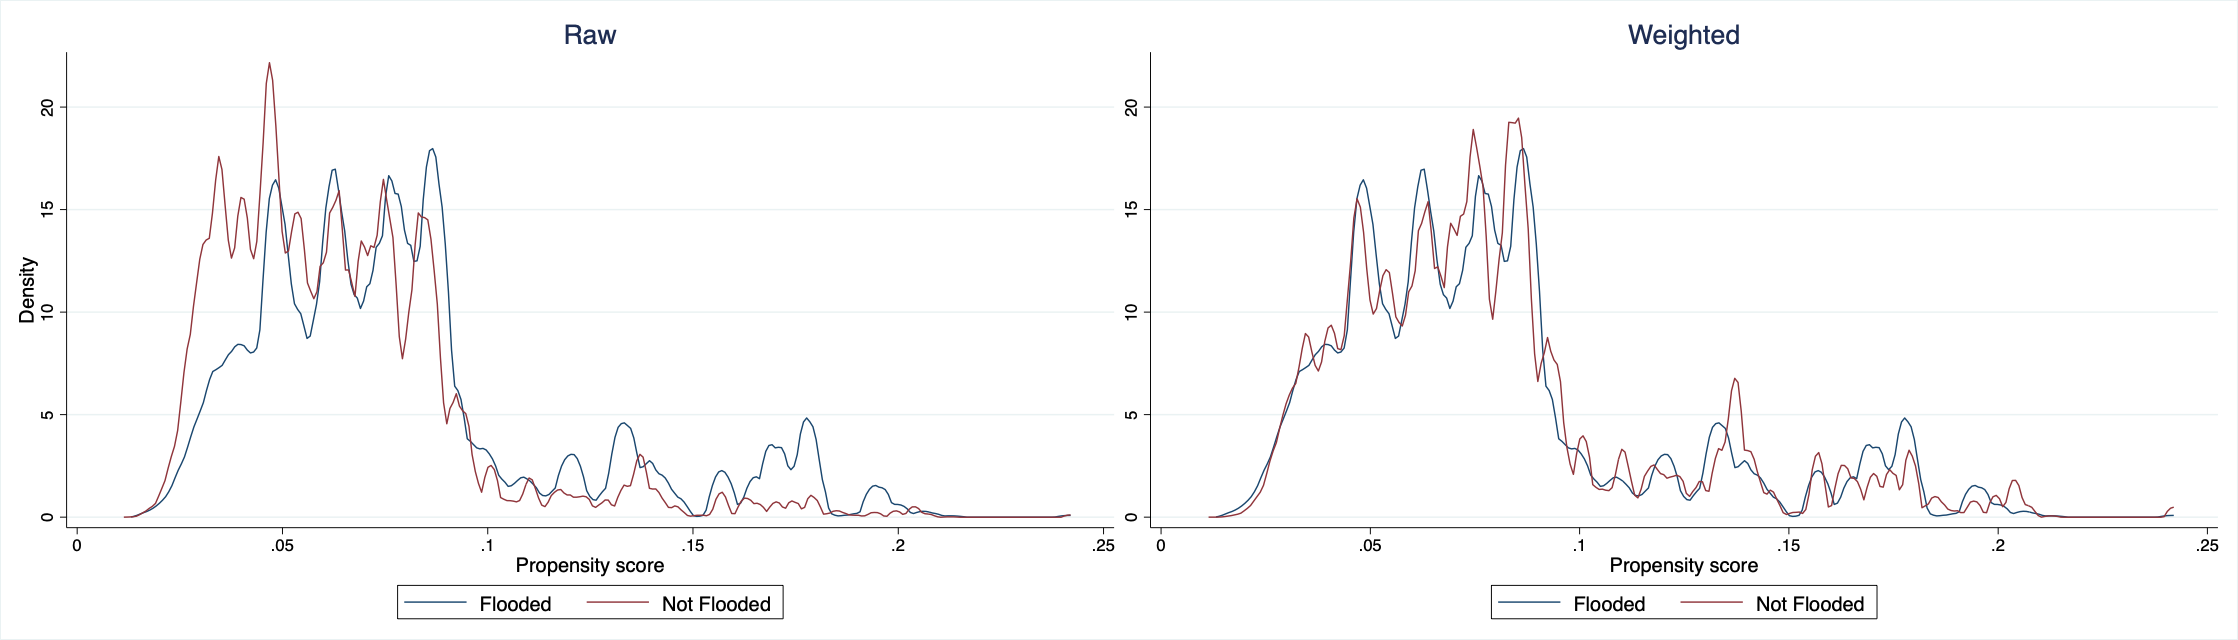
\includegraphics[width=1\textwidth]{figures/PScore/pscore_distrib.png}
\caption*{\raggedright\textit{Note}: The figure displays the distributions of the propensity scores before and after weighting, restricted to the region of common support. 2.12\% of the sample (N=144,299) is excluded because it is not in common support.}
\end{figure}


%%%%%%%%%%%%%%%%%%%%%%%%%%%%%%%%%%%%%%%%%%%%%%%%%%
%%%%%%%%%%%%%%%%%%%%%%%%%%%%%%%%%%%%%%%%%%%%%%%%%%
\clearpage
\section{Additional empirical results}
\label{sec:appendix_empirical}
%%%%%%%%%%%%%%%%%%%%%%%%%%%%%%%%%%%%%%%%%%%%%%%%%%
%%%%%%%%%%%%%%%%%%%%%%%%%%%%%%%%%%%%%%%%%%%%%%%%%%



\begin{table}[htbp]
\centering
\caption{\textbf{Table \ref{tab:stacked_es_employment_wages}:} \textsc{Stacked Event Study Estimates for Employment and Wages}}
\label{tab:stacked_es_employment_wages}


\resizebox{16cm}{!}{
\begin{tabular}{@{\extracolsep{6pt}}p{6.5cm}cccc}
\\[-1.8ex]\hline
\hline \\[-1.8ex]
& \multicolumn{4}{c}{\textit{Dependent variable:}} \\
\cline{2-5}
\\[-1.8ex] 
& \multicolumn{2}{c}{Headcount 31.12} & \multicolumn{2}{c}{Average wage at 31.12} \\
& (1) & (2) & (1) & (2) \\
\hline \\[-1.8ex]
\textbf{A. Post-Treatment Average Effect} \\[0.15em]
Treated $\times$ Post & $-$0.071 & $-$0.150$^{**}$ & $-$135.01$^{***}$ & $-$233.62$^{***}$ \\
                            & (0.045)  & (0.063)         & (41.98)           & (77.57)           \\[0.3em]

\textbf{B. Event-Study Estimates} \\[0.15em]
Treated $\times$ Event-time, $-5$ & $-$0.028 & $-$0.031 & $-$48.52 & $-$16.83 \\
                                 & (0.021)  & (0.033)  & (31.91)  & (48.47)  \\[0.15em]
Treated $\times$ Event-time, $-4$ & 0.008    & 0.027    & $-$52.54$^{**}$ & $-$40.41 \\
                                 & (0.015)  & (0.027)  & (26.37)  & (42.21)  \\[0.15em]
Treated $\times$ Event-time, $-3$ & $-$0.013 & 0.015    & 17.24    & $-$33.38 \\
                                 & (0.014)  & (0.019)  & (25.30)  & (37.73)  \\[0.15em]
Treated $\times$ Event-time, $-2$ & $-$0.013 & $-$0.004 & $-$2.72  & $-$45.89 \\
                                 & (0.013)  & (0.016)  & (25.38)  & (37.39)  \\[0.15em]
Treated $\times$ Event-time, $\phantom{-} 0$  & $-$0.083$^{***}$ & $-$0.169$^{***}$ & $-$186.67$^{***}$ & $-$214.19$^{***}$ \\
                                 & (0.020)         & (0.040)         & (19.88)         & (30.07) \\[0.15em]
Treated $\times$ Event-time, $+1$ & $-$0.114$^{***}$ & $-$0.230$^{***}$ & $-$122.83$^{***}$ & $-$268.61$^{***}$ \\
                                 & (0.036)         & (0.055)         & (27.40)         & (49.05) \\[0.15em]
Treated $\times$ Event-time, $+2$ & $-$0.057$^{*}$   & $-$0.088$^{*}$   & $-$186.74$^{***}$ & $-$236.09$^{***}$ \\
                                 & (0.029)         & (0.045)         & (27.62)         & (62.64) \\[0.15em]
Treated $\times$ Event-time, $+3$ & $-$0.216$^{***}$ & $-$0.144$^{***}$ & $-$165.92$^{***}$ & $-$185.56$^{***}$ \\
                                 & (0.042)         & (0.055)         & (31.77)         & (65.99) \\[0.15em]
Treated $\times$ Event-time, $+4$ & $-$0.132$^{***}$ & $-$0.163$^{***}$ & $-$180.45$^{***}$ & $-$202.26$^{***}$ \\
                                 & (0.034)         & (0.056)         & (38.06)         & (69.77) \\[0.15em]
Treated $\times$ Event-time, $+5$ & $-$0.124$^{**}$  & $-$0.176$^{**}$  & $-$84.79$^{*}$    & $-$187.39$^{**}$  \\
                                 & (0.056)         & (0.082)         & (47.21)         & (80.31) \\[0.35em]


\hline \\[-1.8ex]
Total observations                & 6.82M & 6.82M & 6.82M & 6.82M \\
Variance weighted (stacked) weights               & Yes    & Yes   & Yes    & Yes   \\
ATT weights               & No    & Yes   & No    & Yes   \\
Fixed effects               & Yes   & Yes   & Yes   & Yes   \\
\hline
\hline \\[-1.8ex]
\multicolumn{5}{p{17cm}}{\textit{Note:} Model 1 and Model 2 in parenthesis indicate regression without and with ATT weights, respectively. $^{*}p<0.1$; $^{**}p<0.05$; $^{***}p<0.01$. Event time $-1$ omitted (reference period).}
\end{tabular}}
\end{table}


% EVENT STUDY GRAPHS all outcomes
\begin{figure}[htbp]
  \centering
  \caption{\textbf{Figure \ref{fig:firms_extra_results}:} Impact of floods on firms outcomes - Additional outcomes}
  \label{fig:firms_extra_results}
  
  \begin{subfigure}[t]{0.47\textwidth}
    \centering
    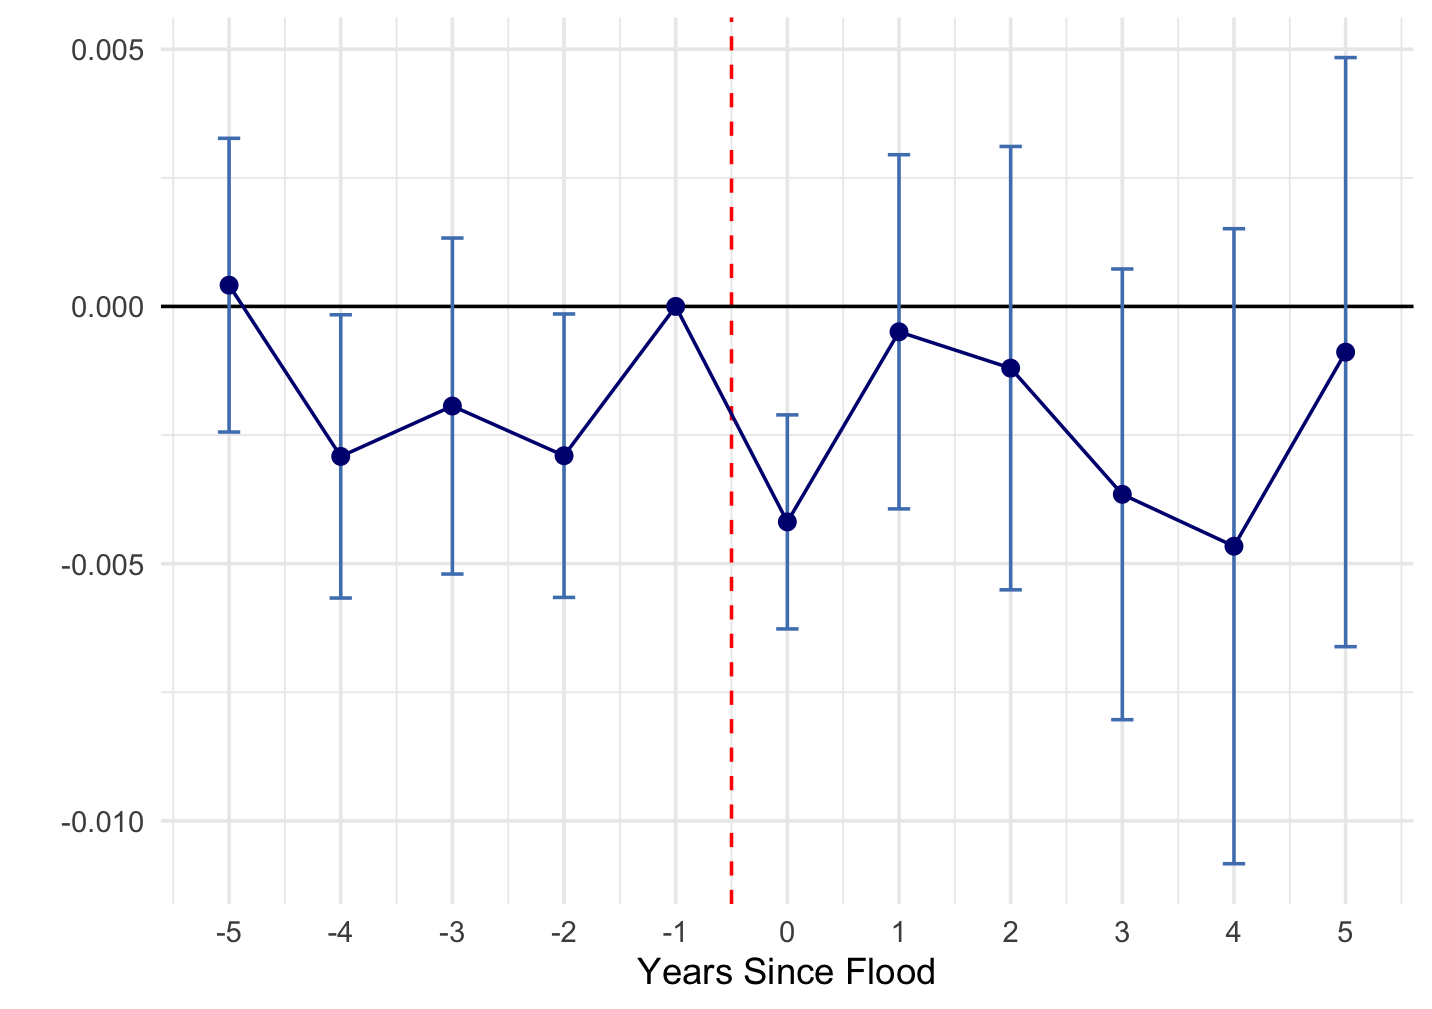
\includegraphics[width=\linewidth]{figures/Results/Analysis_Firms/share_CDD_weighted.png}
    \subcaption{\textbf{Share of temporary contracts}}
  \end{subfigure}
  \hfill
  \begin{subfigure}[t]{0.47\textwidth}
    \centering
    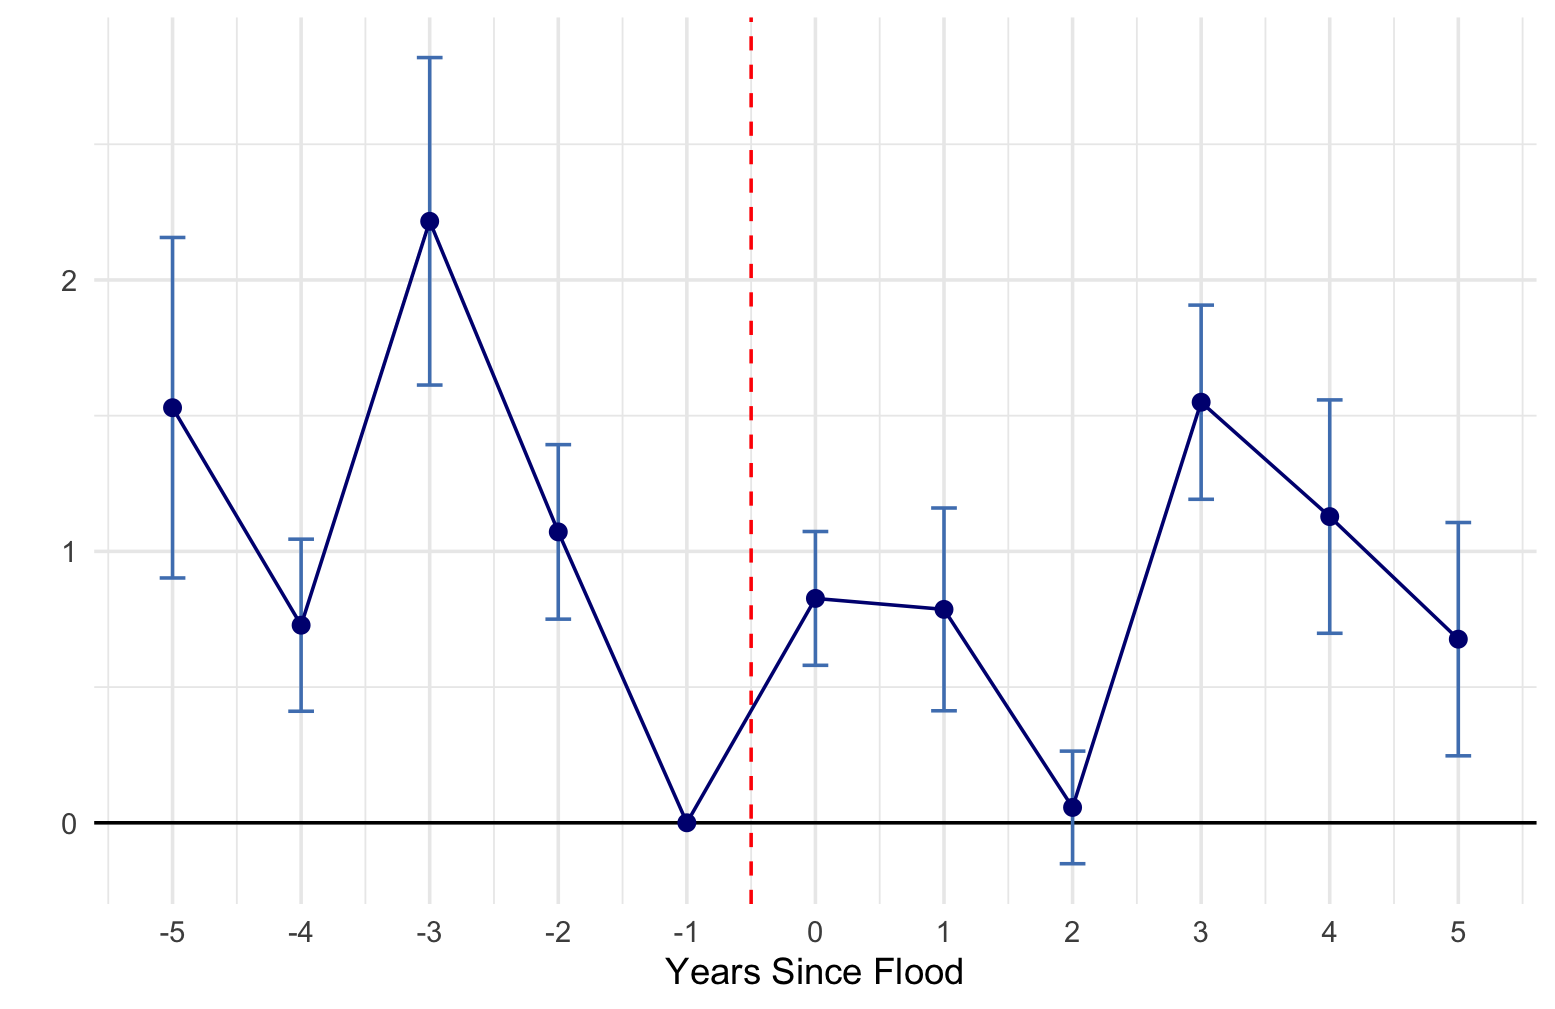
\includegraphics[width=\linewidth]{figures/Results/Analysis_Firms/ETP.png}
    \subcaption{\textbf{FTE Employment}}
  \end{subfigure}

  \vspace{0.8em}

  % Second row

  \begin{subfigure}[t]{0.47\textwidth}
    \centering
    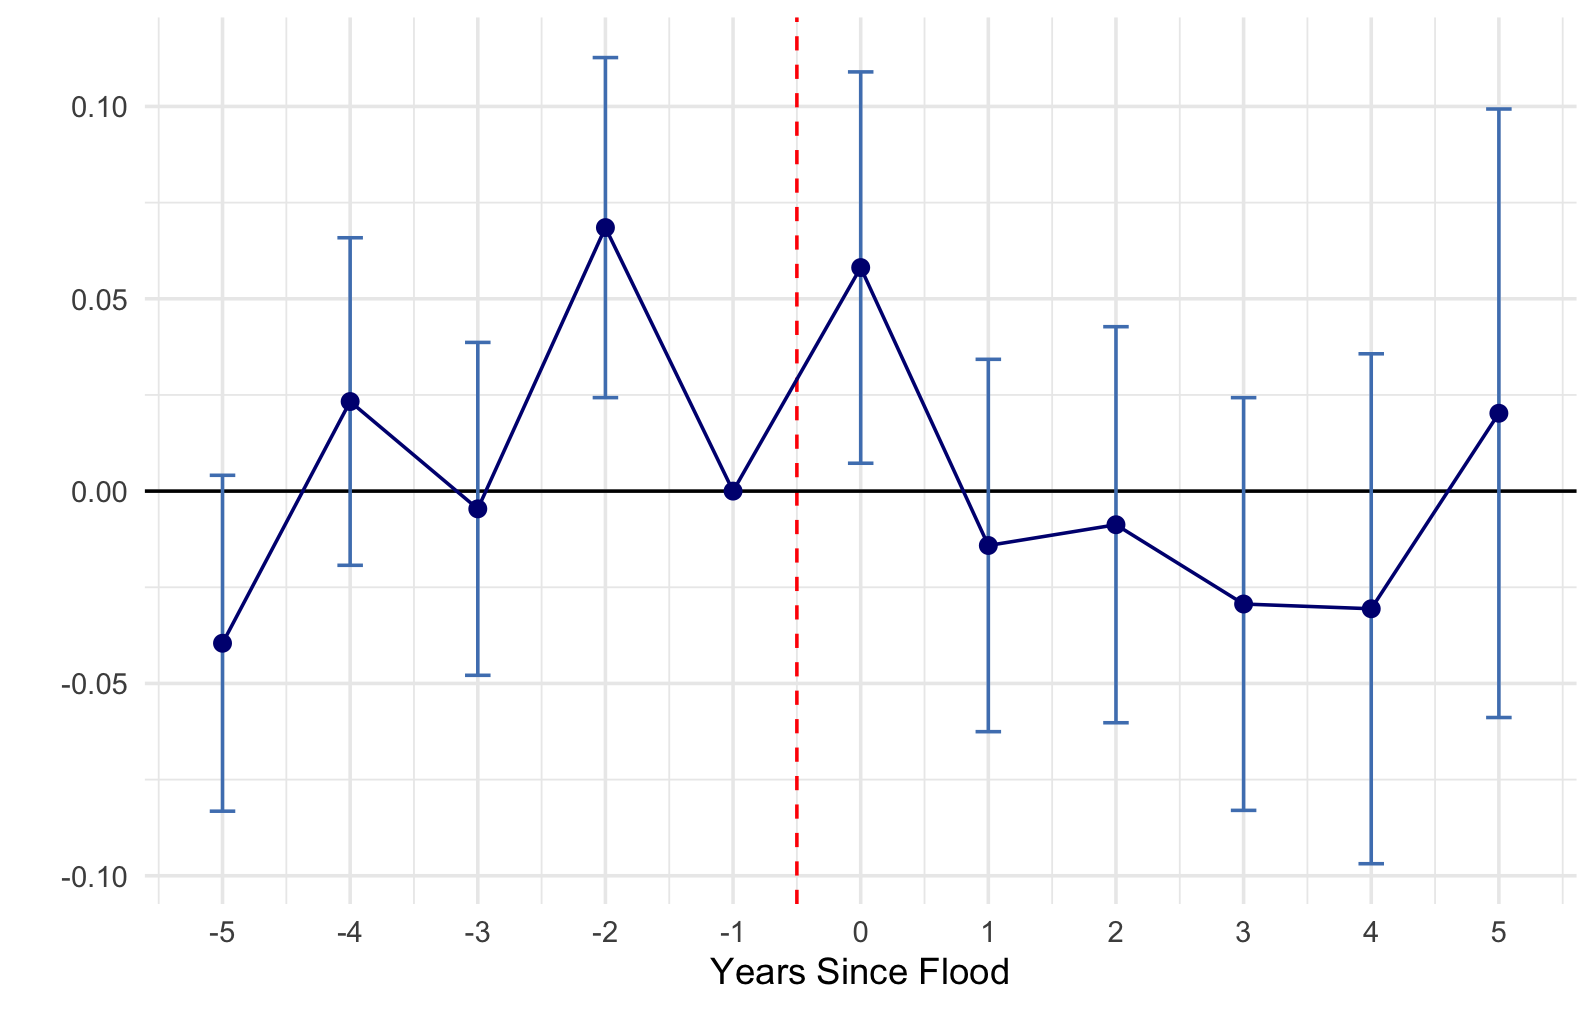
\includegraphics[width=\linewidth]{figures/Results/Analysis_Firms/HWAGE.png}
    \subcaption{\textbf{Hourly Wage}}
  \end{subfigure}
  \hfill
  \begin{subfigure}[t]{0.47\textwidth}
    \centering
    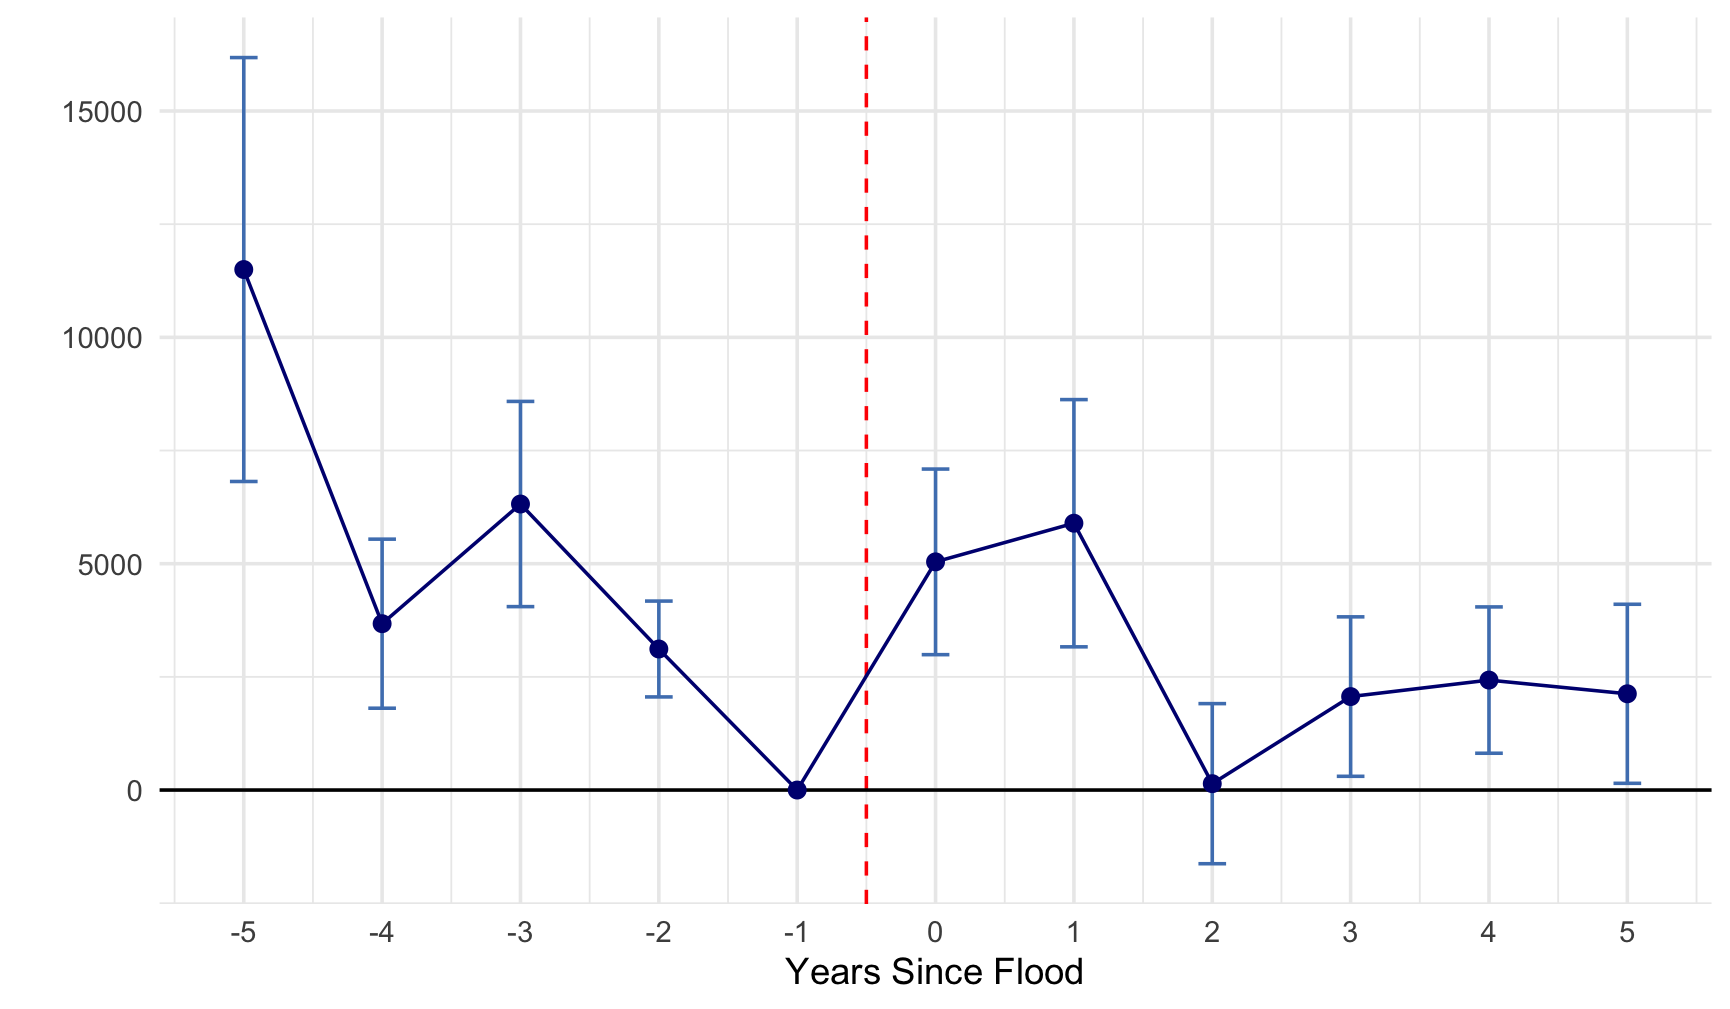
\includegraphics[width=\linewidth]{figures/Results/Analysis_Firms/HOURS.png}
    \subcaption{\textbf{Hours}}
  \end{subfigure}

    \vspace{0.8em}

  % Third row
\begin{subfigure}[t]{0.47\textwidth}
    \centering
    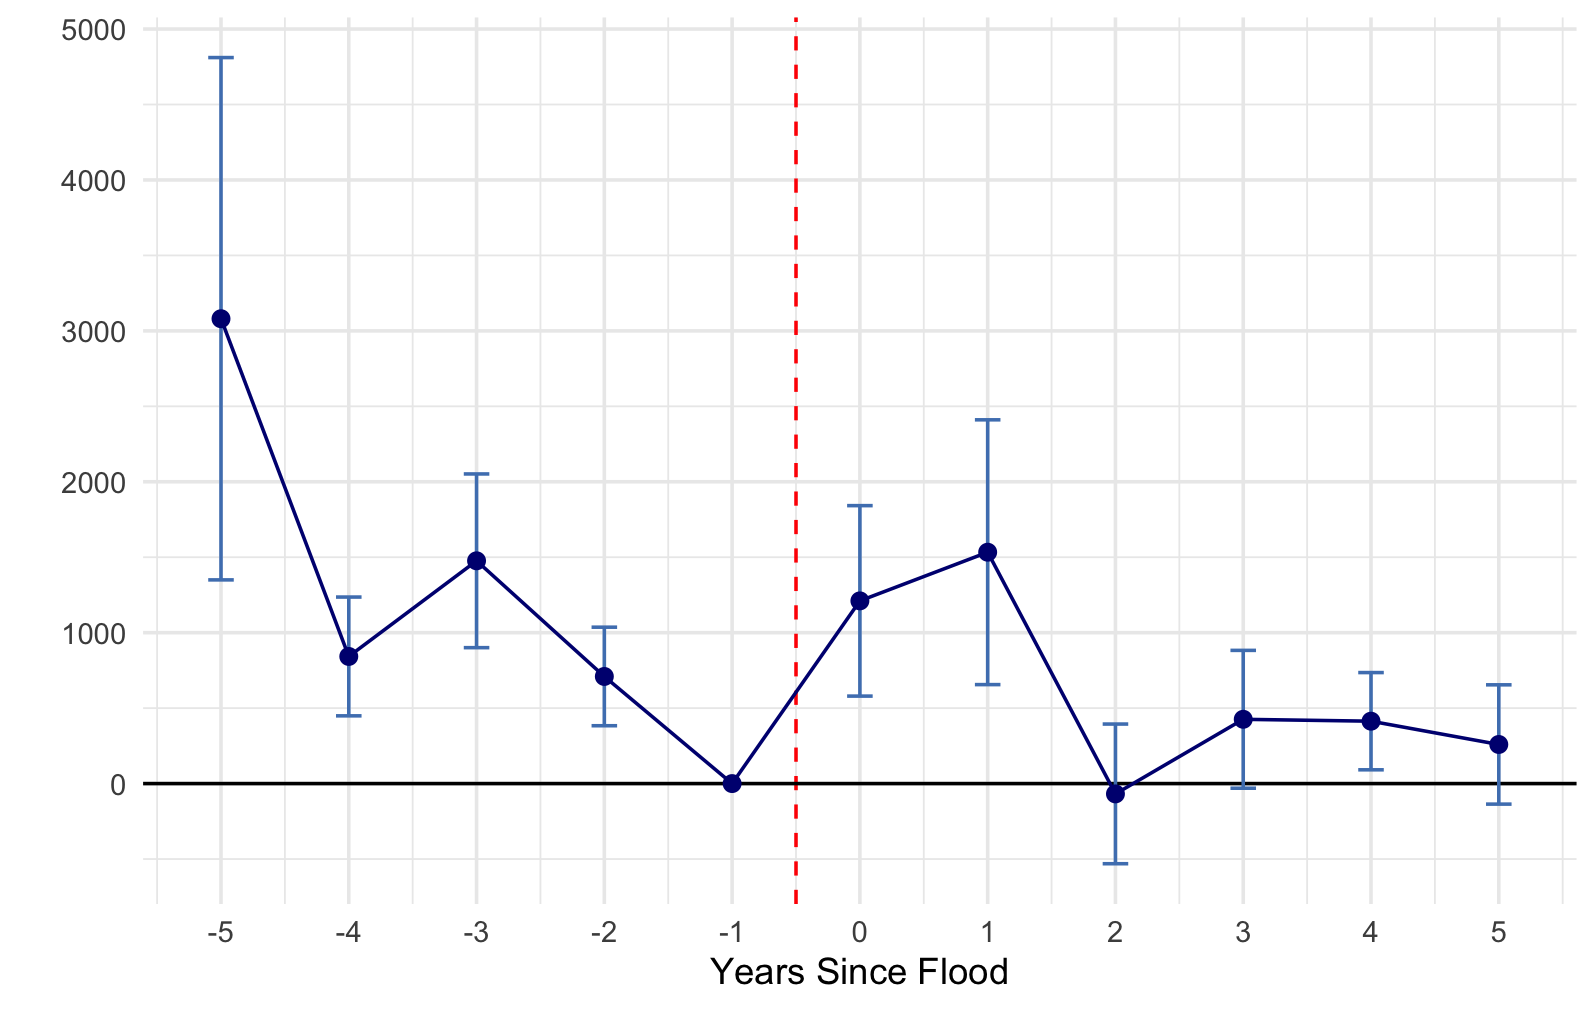
\includegraphics[width=\linewidth]{figures/Results/Analysis_Firms/redi_310_weighted.png}
    \subcaption{\textbf{Total Tunover (Revenue)}}
  \end{subfigure}
  \hfill
  \begin{subfigure}[t]{0.47\textwidth}
    \centering
    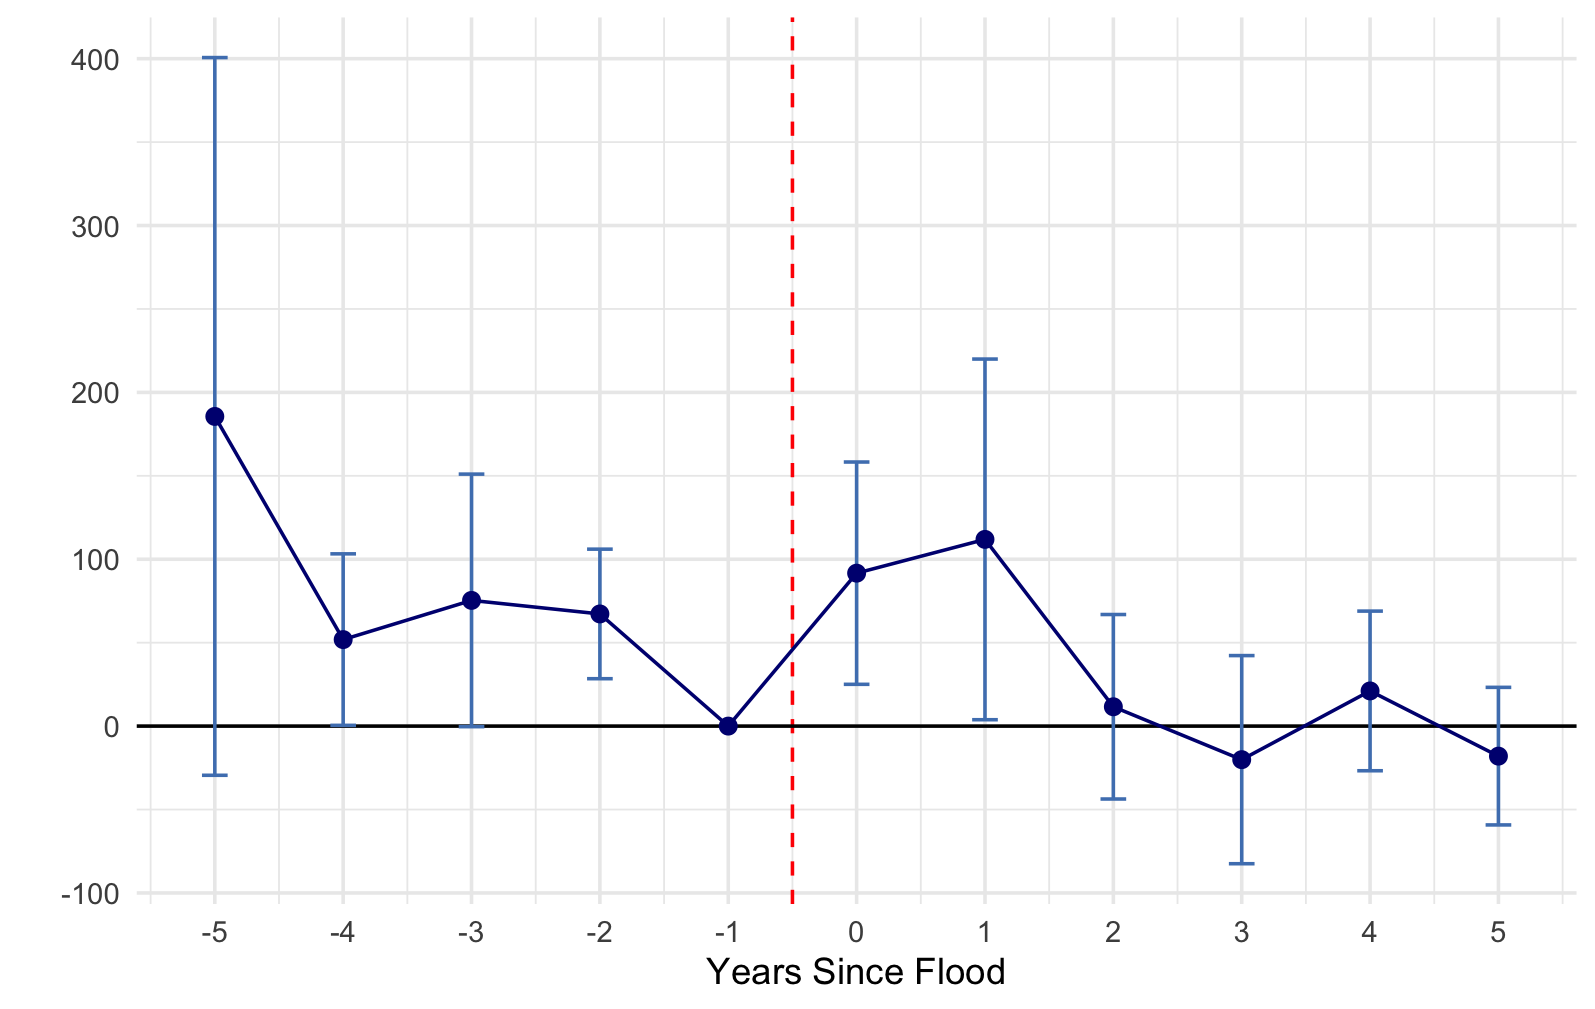
\includegraphics[width=\linewidth]{figures/Results/Analysis_Firms/319 profits.png}
    \subcaption{\textbf{Gross Profit before tax}}
  \end{subfigure}

\end{figure}



%%%%%%%%%%%%%%%%%%%%%%%%%%%%%%%%%%%%%%%%%%%%%%%%%%
%%%%%%%%%%%%%%%%%%%%%%%%%%%%%%%%%%%%%%%%%%%%%%%%%%
\clearpage
\section{Additional tables}
\label{sec:appendix_tables}
%%%%%%%%%%%%%%%%%%%%%%%%%%%%%%%%%%%%%%%%%%%%%%%%%%
%%%%%%%%%%%%%%%%%%%%%%%%%%%%%%%%%%%%%%%%%%%%%%%%%%



% Table - Flood Events count
\begin{table}[htbp]
  \centering
  \caption{\textbf{Table \ref{tab:flood_summary}:} History of flood events, affected communes and firms}
  \label{tab:flood_summary}
  \resizebox{\textwidth}{!}{%
  \begin{threeparttable}[b]
    \begin{tabular}{l r r r r r r r r}
      \toprule\toprule
      & \multicolumn{1}{c}{\textbf{CatNat decrees}} 
      & \multicolumn{1}{c}{\textbf{Communes affected}} 
      & \multicolumn{6}{c}{\textbf{Firms in sample}}\\[-0.2em]
      \cmidrule(lr){4-9}
      Year 
      & 
      & 
      & \multicolumn{3}{c}{Flooded}
      & \multicolumn{3}{c}{Total SIRETs} \\
      \cmidrule(lr){4-6} \cmidrule(lr){7-9}
      & & 
      & \multicolumn{1}{c}{$<$1 day} 
      & \multicolumn{1}{c}{1–22 days} 
      & \multicolumn{1}{c}{$>$22 days} 
      & \multicolumn{1}{c}{Affected} 
      & \multicolumn{1}{c}{Non-Affected} 
      & \multicolumn{1}{c}{Flood rate (\%)}\\
      \midrule
      2000 & 33 & 2\,227 & -- & -- & -- & -- & -- & -- \\
      2001 & 42 & 2\,879 & -- & -- & -- & -- & -- & -- \\
      2002 & 27 & 1\,163 & -- & -- & -- & -- & -- & -- \\
      2003 & 27 & 2\,261 & -- & -- & -- & -- & -- & -- \\
      2004 & 19 &   334 & -- & -- & -- & -- & -- & -- \\
      2005 & 21 &   842 & -- & -- & -- & -- & -- & -- \\
      2006 & 24 & 1\,072 & -- & -- & -- & -- & -- & -- \\
      2007 & 19 & 1\,070 & -- & -- & -- & -- & -- & -- \\
      2008 & 26 & 2\,177 & -- & -- & -- & -- & -- & -- \\
      2009 & 23 & 4\,425 & -- & -- & -- & -- & -- & -- \\
      2010 & 23 & 1\,981 & 24\,107 & 43\,415 & 0     & 67\,522 & 587\,707 & 10.31 \\
      2011 & 23 &   962 & 25\,834 & 35\,847 & 0     & 61\,681 & 669\,845 & 8.43 \\
      2012 & 18 &   729 & 16\,350 & 11\,930 & 21    & 28\,301 & 635\,386 & 4.26 \\
      2013 & 31 & 1\,511 & 29\,098 & 40\,948 & 145   & 70\,191 & 607\,992 & 10.35 \\
      2014 & 33 & 2\,057 & 26\,898 & 82\,310 & 129   & 109\,337 & 609\,840 & 15.20 \\
      2015 & 22 &   776 & 48\,124 & 12\,579 & 2     & 60\,705 & 629\,434 & 8.80 \\
      2016 & 29 & 2\,846 & 28\,609 & 61\,608 & 21    & 90\,238 & 546\,372 & 14.17 \\
      2017 & 23 &   303 & 15\,063 & 2\,017  & 0     & 17\,080 & 666\,863 & 2.50 \\
      2018 & 37 & 3\,426 & 76\,373 & 96\,275 & 753   & 173\,401 & 663\,240 & 20.73 \\
      2019 & 26 &   913 & 29\,246 & 63\,188 & 0     & 92\,434 & 728\,887 & 11.26 \\
      2020 & 28 & 1\,168 & -- & -- & -- & -- & -- & -- \\
      \bottomrule\bottomrule
    \end{tabular}
    \begin{tablenotes}[flushleft]
      \small
      \item \emph{Notes:} “Affected” firms are disaggregated by flood duration: less than 1 day (low), 1–22 days, and $>$22 days (high). The flood rate (\%) is the share of affected firms over the total observed firms in a given year.
    \end{tablenotes}
  \end{threeparttable}}
\end{table}



% Table: Flood counts 2000-2020
% \begin{table}[htbp]
  \centering
  \caption{\textbf{Table \ref{tab:flood_counts}}: Flood statistics (2000-2020)}
  \label{tab:flood_counts}
  \resizebox{0.8\textwidth}{!}{%
  \begin{threeparttable}[b]
    \begin{tabular}{lrrrrr}
      \toprule\toprule
      Total floods & SIRETs & $<$ 1 day & 1 to 22 days & $>$ 22 days & Avg. years between \\
      \midrule
      0 & 1\,884\,703 & -- & -- & -- & -- \\
      1 & 625\,619 & 285\,690 & 339\,106 & 823 & -- \\
      2 & 150\,801 & 145\,024 & 156\,381 & 197 & 3.69 \\
      3 & 45\,475 & 66\,798 & 69\,588 & 39 & 3.29 \\
      4 & 18\,178 & 33\,148 & 39\,555 & 9 & 2.74 \\
      5 & 7\,820 & 16\,941 & 22\,157 & 2 & 2.62 \\
      6 & 2\,423 & 5\,614 & 8\,923 & 1 & 2.41 \\
      7 & 723 & 1\,903 & 3\,158 & 0 & 2.08 \\
      8 & 189 & 562 & 950 & 0 & 1.95 \\
      9 & 81 & 183 & 546 & 0 & 1.74 \\
      \midrule
      Total & 2\,736\,012 & 555\,863 (20.32\%) & 640\,364 (23.41\%) & 1\,071 (0.04\%) & -- \\
      \bottomrule\bottomrule
    \end{tabular}%
    \begin{tablenotes}[flushleft]
      \small
      \item \emph{Notes:} Data aggregated from flood exposure at the SIRET level. Percentages in parentheses represent the proportion of SIRETs affected by each flood intensity relative to total SIRETs.
    \end{tablenotes}
  \end{threeparttable}%
  }
\end{table}


% Table: Flood counts 2010-2019
\vspace{1cm}
\begin{table}[htbp]
  \centering
  \caption{\textbf{Table \ref{tab:flood_counts19}}: Flood statistics (2010--2019)}
  \label{tab:flood_counts19}
  \resizebox{0.8\textwidth}{!}{%
  \begin{threeparttable}[b]
    \begin{tabular}{lrrrrr}
      \toprule\toprule
      Total floods & SIRETs & Low (1 day) & Medium (1–22 days) & High ($>$22 days) & Avg. years between \\
      \midrule
      0 & 1\,455\,888 & -- & -- & -- & -- \\
      1 & 445\,886 & 180\,317 & 264\,724 & 845 & -- \\
      2 & 95\,527 & 80\,767 & 110\,084 & 203 & 1.39 \\
      3 & 27\,988 & 37\,561 & 46\,380 & 23 & 1.34 \\
      4 & 9\,592 & 16\,628 & 21\,740 & 0 & 1.30 \\
      5 & 1\,799 & 3\,469 & 5\,526 & 0 & 1.28 \\
      6 & 422 & 929 & 1\,603 & 0 & 1.24 \\
      7 & 13 & 31 & 60 & 0 & 1.06 \\
      \midrule
      Total & 2\,037\,115 & -- & -- & -- & -- \\
      %Total & 2\,037\,115 & 239\,702 (11.8\%) & 449\,117 (22.0\%) & 1\,071 (0.05\%) & -- \\
      \bottomrule\bottomrule
    \end{tabular}
    \begin{tablenotes}[flushleft]
      \small
      \item \emph{Notes:} Flood counts refer to the number of floods experienced by a commune between 2010 and 2019. Low/Medium/High intensity is based on total duration of the CatNat decree.
    \end{tablenotes}
  \end{threeparttable}
  }
\end{table}

% Table: SIRET YEARS
\begin{table}[htbp]
  \centering
  \caption{\textbf{Table \ref{tab:n_years_firms}}: Number of Years Firms Appear in the Data (2010--2019)}
  \label{tab:n_years_firms}
  \resizebox{0.5\textwidth}{!}{%
    \begin{threeparttable}[b]
      \begin{tabular}{cccc}
        \toprule\toprule
        Years Present & Frequency & Percent & Cumulative \\
        \midrule
        1  & 600,750  & 8.81  & 8.81  \\
        2  & 840,246  & 12.32 & 21.13 \\
        3  & 842,433  & 12.35 & 33.48 \\
        4  & 829,720  & 12.16 & 45.64 \\
        5  & 720,665  & 10.57 & 56.21 \\
        6  & 694,524  & 10.18 & 66.39 \\
        7  & 513,807  & 7.53  & 73.92 \\
        8  & 511,576  & 7.50  & 81.42 \\
        9  & 364,680  & 5.35  & 86.77 \\
        10 & 902,460  & 13.23 & 100.00 \\
        \midrule
        Total & 6,820,861 & 100.00 & -- \\
        \bottomrule\bottomrule
      \end{tabular}
      \begin{tablenotes}[flushleft]
        \small
        \item \emph{Notes:} This table shows how many years (out of 10 between 2010 and 2019) each SIRET appears in the data. Approximately 13\% of firms are present for the full decade.
      \end{tablenotes}
    \end{threeparttable}
  }
\end{table}



% Table - LOnger results
%\begin{table}[!htbp]
\centering
\caption{\textbf{Table \ref{tab:lpdid_results}:} \textsc{OLD TABLE -- LP-DiD event-study estimates with bin-level observations}}
\label{tab:lpdid_results}

\resizebox{14.5cm}{!}{
\begin{tabular}{@{\extracolsep{6pt}}p{8cm}ccr}
\\[-1.8ex]\hline
\hline \\[-1.8ex]
& \multicolumn{2}{c}{\textit{Dependent variable:}} & \\
\cline{2-3}
\\[-1.8ex] & EFF\_3112 (Employment) & AVGWAGE\_3112 (Wages) & Obs (bin) \\
\hline \\[-1.8ex]
Event time $-5$ & $-$0.031 & $-$16.83 & 521,227 \\
                & (0.033)  & (48.47)  &         \\[0.15em]
Event time $-4$ & 0.027    & $-$40.41 & 650,620 \\
                & (0.027)  & (42.21)  &         \\[0.15em]
Event time $-3$ & 0.015    & $-$33.38 & 794,878 \\
                & (0.019)  & (37.73)  &         \\[0.15em]
Event time $-2$ & $-$0.004 & $-$45.89 & 989,096 \\
                & (0.016)  & (37.39)  &         \\[0.15em]
Event time $-1$ & 0 (reference) & 0 (reference) & -- \\ [0.15em]
Event time $0$  & $-$0.169$^{***}$ & $-$214.19$^{***}$ & 1,369,029 \\
                & (0.040)         & (30.07)            &            \\[0.15em]
Event time $1$  & $-$0.230$^{***}$ & $-$268.61$^{***}$ & 807,004 \\
                & (0.055)         & (49.05)            &         \\[0.15em]
Event time $2$  & $-$0.088$^{*}$   & $-$236.09$^{***}$ & 585,341 \\
                & (0.045)         & (62.64)            &         \\[0.15em]
Event time $3$  & $-$0.144$^{***}$ & $-$185.56$^{***}$ & 442,005 \\
                & (0.055)         & (65.99)            &         \\[0.15em]
Event time $4$  & $-$0.163$^{***}$ & $-$202.26$^{***}$ & 322,004 \\
                & (0.056)         & (69.77)            &         \\[0.15em]
Event time $5$  & $-$0.176$^{**}$  & $-$187.39$^{**}$  & 224,432 \\
                & (0.082)         & (80.31)            &         \\[0.35em]

\hline \\[-1.8ex]
Total observations     & 1,369,029 & 1,237,240 & -- \\
Mean per bin           & 676,977   & 608,899   & -- \\
\hline
\hline \\[-1.8ex]
\multicolumn{4}{p{17cm}}{\textit{Note:} Cluster-robust standard errors (at the INSEE\_COM level) in parentheses. $^{*}p<0.1$; $^{**}p<0.05$; $^{***}p<0.01$. Event time $-1$ is the omitted reference category.} \\[0.6em]

\multicolumn{4}{p{17cm}}{\texttt{lpdid(Y, unit = SIRET, time = ANNEE, treat = flood\_dummy\_extreme, pre\_window = 5, post\_window = 5, controls = c(floods\_last\_10y, floods\_last\_5y, floods\_last\_3y, years\_since\_last\_flood), cluster = INSEE\_COM, absorb = i.flood\_risk\_group\#i.Section\#\#c.ANNEE, weights = w\_att)}}
\end{tabular}}
\end{table}








%\subsection{Establishment-level data}


%\section{Robustness Checks}


\begin{landscape}
\scriptsize
\begin{ThreePartTable}
\begin{TableNotes}[flushleft]\footnotesize
%\item \textit{Note:} PCS-based variables are constructed by .
\end{TableNotes}

\begin{longtable}{@{}p{9cm}p{9cm}@{}}
\caption{\textbf{Table \ref{tab:codebook}:} Variable Codebook, FARE-FICUS and DADS}\label{tab:codebook}\\
\toprule
\textbf{Variable} & \textbf{Description} \\
\midrule
\endfirsthead
\multicolumn{2}{l}{\textbf{(Continued)}}\\
\toprule
\textbf{Variable} & \textbf{Description} \\
\midrule
\endhead

\bottomrule
\insertTableNotes
\endlastfoot

% --- FARE–FICUS ---
\multicolumn{2}{l}{\textit{FARE–FICUS dataset}}\\[0.2em]
\texttt{SIREN}            & Legal-unit identifier\\
\texttt{ANNEE}            & Calendar year\\
\texttt{depcom}           & Commune code (head office)\\
\texttt{ape\_diff}        & Main activity (NAF Rev. 1)\\
\texttt{r004}             & VAHT – IMPOTAX + SUBVEXP (value added)\\
\texttt{redi\_e001}       & Headcount on 31 Dec\\
\texttt{redi\_e200}       & Average salaried headcount (EFFSALM)\\
\texttt{redi\_r310}       & Total turnover (CATOTAL)\\
\texttt{redi\_r216}       & Wages and salaries (SALTRAI)\\
\texttt{b319}             & Current gross profit before tax (PBCAI)\\
\texttt{b330}             & Loans and related debts (EMPDETT)\\
\texttt{CAPISOC}          & Share capital\\
\texttt{VAHT}             & Value added excl. tax\\
\texttt{IMPOTAX}          & Taxes and duties\\
\texttt{SUBVEXP}          & Operating subsidies\\[0.5em]

% --- DADS ---
\multicolumn{2}{l}{\textit{DADS dataset}}\\[0.2em]
\texttt{YEAR}             & Calendar year\\
\texttt{SIREN}            & Legal-unit identifier\\
\texttt{SIRET}            & Establishment identifier\\
\texttt{ZEMPT}            & Employment-zone code\\
\texttt{Code\_commune}    & INSEE commune code (establishment)\\[0.5em]

% --- PCS aggregates ---
\multicolumn{2}{l}{\textit{PCS-based aggregates (available by socio-professional category)}}\\[0.2em]
\texttt{EFF\_ALL}         & Total salaried employment\\
\texttt{HOURS}            & Total hours worked\\
\texttt{HWAGE}            & Mean hourly wage\\
\texttt{AVGWAGE}          & Mean annual wage\\
\texttt{ETP}              & Full-time equivalents\\
\texttt{EFF\_3112}        & Headcount on 31 Dec (establishment level)\\ [0.5em]

% --- Employment dynamics ---
\multicolumn{2}{l}{\textit{Employment dynamics}}\\[0.2em]
\texttt{HIRES}            & Hires during year\\
\texttt{HIRES2}           & Alternative hires definition\\
\texttt{SEPARATIONS}      & Separations during year\\[0.5em]

% --- Contract shares ---
\multicolumn{2}{l}{\textit{Contract-type shares}}\\[0.2em]
\texttt{CDI}              & Share of open-ended contracts\\
\texttt{CDD}              & Share of fixed-term contracts\\
\texttt{interim}          & Share of temporary-agency contracts\\
\texttt{othercontract}    & Share of other contract types\\[0.5em]

% --- Short contracts ---
\multicolumn{2}{l}{\textit{Job spell by duration}}\\[0.2em]
\texttt{SHORTJOB\_1M}     & $\leq$ 1 month\\
\texttt{SHORTJOB\_3M}     & $\leq$ 3 months\\
\texttt{SHORTJOB\_6M}     & $\leq$ 6 months\\
\texttt{SHORTJOB\_LTO3M}  & $<$ 3 months\\
\texttt{SHORTJOB\_3TO6M}  & 3–6 months\\
\texttt{SHORTJOB\_6TO12M} & 6–12 months\\
\texttt{SHORTJOB\_MORE6M} & $>$ 6 months\\
\texttt{SHORTJOB\_MORE1Y} & $>$ 1 year\\

\end{longtable}
\end{ThreePartTable}
\end{landscape}



\end{document}








